\documentclass{article}
\usepackage[utf8]{inputenc}
\usepackage[L7x]{fontenc}
\usepackage[lithuanian]{babel}
\usepackage{lmodern}
\usepackage{amsmath}
\usepackage{graphicx}
\usepackage{verbatim}
\usepackage{hyperref}
\usepackage{subfigure}
\usepackage{tcolorbox}
\usepackage{mdframed}
\usepackage{tikz}
\usepackage{color}
\usepackage{cancel}
\usepackage[top=2cm, bottom=2cm, left=2cm, right=2cm, footskip=1cm, a4paper]{geometry}

\usepackage{hyperref}
\usepackage[upint]{stix}
\begin{document}
\tableofcontents{}
\newcommand{\DrawCard}[2]{\begin{tikzpicture}[scale=1.5, baseline=-0.7ex]\node[red,draw=blue, rounded corners=.2cm, line width=0.5628571428571mm, fill=#2] (leaf1) at  (0.0, 0.0)  {$\colorbox{#2}{#1}$};\end{tikzpicture}}
\begin{comment}
Elzė Sigutė Mikalonytė atlieka muzikos sąvokų (kyla, leidžiasi, tolsta, artėja, platėja, siaurėja) tyrimą
\end{comment}
\newtcolorbox{mybox}[1]{colback=red!5!white,colframe=red!75!black,fonttitle=\bfseries,title=#1}

\newpage
\section{Matematikos ugdymas edukologijos požiūriu}
\subsection{Esminis matematikos ugdymo išsiskyrimas iš kitų dalykų ugdymo}
Šiame skyriuje pacituosime dėstytojo Rimo Norvaišos nuomonę.

Vaizdžiai kalbant, mūsų pedagogika (edukologija, didaktika ir t.t.) nešioja akinius skirtus žiūrėti į tolį. Norint pamatyti mūsų mokyklinės matematikos problemas, reikia užsidėti akinius skaitymui.

Ką tai reiškia? Priklausomai nuo akinių tipo matematikos žinios vertinamos skirtingai. Bendroji pedagogika ir mokslo pedagogika matematikos žinias ir gebėjimus matuoja naudodama Bloom'o taksonomiją (vėliau Andersono pakoreguota). Ši taksonomija suklasifikuoja žinias į lygmenis: 
\begin{enumerate}
\item įsiminimas 
\item supratimas 
\item taikymas
\item analizė
\item vertinimas
\item kūrimas
\end{enumerate}
Šiais žinių lygmenimis yra įprasta vertinti mokyklines humanitarines ir gamtos mokslų žinias. Tačiau jos yra per daug grubios vertinti matematikos žinias. Pagal Bloom'o klasifikaciją neįmanoma atskirti algoritmų išmokimą, nuo jų supratimo. Šis sutapatinimas yra mūsų mokyklinės matematikos Achilo kulnas.

Mokyklinės matematikos žinioms vertinti naudojamas skirstymas į 
\begin{itemize}
\item faktines žinias (atsiminimas)
\item procedūrines žinias (gebėjimas naudotis algoritmais)
\item sąvokines žinios (gebėjimas suprasti).
\end{itemize} 

Tai yra ,,akiniai skaitymui" pakankami įžvelgti mokyklinės matematikos sunkumus.

Pastaroji klasifikacija naudojama srityje, kuri pasaulyje vadinama ,,mathematics education" ir yra tarp kitų matematikos sričių pagal standartinę mathematics subject classification. Lietuvoje panašiu pavadinimu, ,,matematikos didaktika", yra mokslo ir bendrosios pedagogikos taikymas matematikai. Mes turime ne vieną didaktikos profesionalą. Bet neturime nei vieno ,,mathematics education" profesionalo.

\subsection{Pavyzdžiai, iliustruojantys matematinio ugdymo problemų mastą}
Pagal vykdomus mokinių pasiekimo tyrimus mokinių \textbf{matematinio raštingumo} lygis Lietuvos mokyklose yra žemas. 

\textbf{Pirmas pavyzdys.} Rusų mokyklose sprendžiamas antros klasės uždavinys ir uždavinys mūsų šalies mokyklose, kurį mūsų moksleiviai sprendžia ne anksčiau, nei penktoje klasėje:

\includegraphics[width=0.7\textwidth]{ruvslt.jpg}

\textbf{Antras pavyzdys.} „Man teko susipažinti su Latvijos, Škotijos, Lenkijos ir Rusijos matematikos brandos egzaminais ir turiu pažymėti, kad visose šalyse matematikos egzaminas sunkesnis ir gerokai sudėtingesnis nei Lietuvoje“, – žurnale ,,Reitingai'' cituojama matematikos mokytojų asociacijos prezidentė Regina Rudalevičienė.

\textbf{Trečias pavyzdys.}
Lietuvos matematikos mokymo sistema (kaip ir Airijos, Graikijos, Ispanijos, Latvijos, Portugalijos ir Rumunijos) 2009 metais PISA apklausos įvertinta blogiau už Europos Sąjungos vidurkį. Nustatyta, kad $26,3\%$ moksleivių matematinis raštingumas yra žemas.

\subsection{Galimos matematikos ugdymo problemų priežastys}

Kodėl mūsų šalies mokinių rezultatai matematikoje tokie prasti? Tiesioginiai prastus rezultatus lemiantys veiksniai galėtų būti:
\begin{itemize}
\item Nėra tikrinamos moksleivių sąvokinės matematikos žinios.
\item Žemi matematinio ugdymo standartai, atsispindintys egzaminų užduotyse ir vadovėliuose.
\item Mokytojų nesupažindinimas su elementariąja matematika matematinio samprotavimo požiūriu (kitaip tariant, būsimi ir esami mokytojai neturi pakankamų gebėjimų paaiškinti matematikos procedūras (apie problemą kalbama poskyryje ,,Vystymosi raidos taikymas matematikos ugdyme''; praktinės užduotys siūlomos skyriuje ,,Kaip mokyti matematikos'')
\item Klaidingai formuluojamas dabartinio matematinio ugdymo tikslas (žr. kitą poskyrį): 
\end{itemize}
Netiesioginiai veiksniai:
\begin{itemize}
\item \textbf{Mokinių tėvų vaidmuo}
\begin{itemize}
\item Tėvų neinformuotumas apie mokyklos veiklą: žemas mūsų šalies matematikos (ir ne tik) lygis suvokiamas kaip smulkios klaidelės egzaminuose ar vadovėliuose, manoma, kad matematikos ugdymo lygis nepakito nuo ankstesnės kartos laikų.
\item Kelių kartų susiformavęs požiūris į matematiką kaip į sunkų, sausą ir su gyvenimu nesusijusį mokslą, lemiantis dabartinės jaunosios kartos motyvaciją (jei įmanoma – vengti) mokantis matematikos.
\item Tėvų diegiamas vaikams įspūdis apie matematiką, kaip muštro ir paklusnumo priemonę, neturinčią bendrų ryšių su pasaulio pažinimu. Plačiau apie šio reiškinio pasekmes skyriuje \hyperlink{mspp}{\textit{\textbf{Mokymosi specifika psichologijos požiūriu}}}
\end{itemize}
\item \textbf{Pedagogų vaidmuo} Krenta į akis per didelis susižavėjimas kompetencijomis, mokymąsi suvokiant tarsi būdą gauti kurią nors kompetenciją. Taip traktuojant ugdymą, dingsta tiek matematikos vidiniai ryšiai, tiek matematikos ryšiai su kitais mokslais. 
\item \textbf{Mokinių vaidmuo}
\begin{itemize}
\item Didelė moksleivių dalis mokymąsi supranta kaip pramogą, jie nepasiruošę sunkiai dirbti ir neturi motyvacijos mokytis matematikos, likusi moksleivių dalis ir mokytojai skundžiasi per mažu pamokų skaičiumi.
\item Daugumai mokinių matematika kelia baimės jausmą.  Akivaizdu, jog svarbiausia to priežastimi yra matematikos hierarchinė struktūra. Viena nesuprasta sąvoka ar procedūra trukdo įsisavinti kitas nuo jos priklausančias sąvokas  ar procedūras. Nesupratimas kaupiasi ir tampa panašiu į sniego gniūžtės efektą. Matematikos simbolinės kalbos nesupratimas įvardijamas kitu moksleivių baimės šaltiniu.    
\item Nemažą įtaką motyvacijai mokytis  matematiką, nesėkmėms bei baimės jausmui mokantis matematikos  daro ir socialiniai stereotipai: esą, matematikai  suprasti  reikia  įgimtų  gabumų; berniukų  mąstymas,  lyginant  jį  su  mergaičių  mąstymu,  yra  geriau  suderinamas  su  abstrakčiu mąstymu
\item Neatsakingas skaičiuotuvų, išmaniųjų programėlių ir kompiuterių naudojimas mažina poreikį mokytis matematikos. ,,PhotoMath'' programėlės pavyzdys parodo, kad matematikos mokytis nereikalinga, nes kompiuteris gali išspręsti beveik bet kurį aritmetinį mokyklinės matematikos uždavinį.
\end{itemize}
\item \textbf{Visuomenės vaidmuo} Visuomenė neturi minimalių žinių apie šiuolaikinės matematikos prigimtį ir matematikos vaidmenį šiuolaikiniame pasaulyje. Tai nulemia jos nenorą nujausti pokyčių prasmę, t.y. nenorą keisti dabartinį matematikos mokymą. 
\end{itemize}

\subsection{Klaidingai keliamas matematikos ugdymo tikslas}
Apibendrinant ankstesnį skyrelį galima pasakyti, kad \textbf{pagrindinė problema} yra matematikai būdingo samprotavimų loginio tikslumo nebuvimas mokyklinės matematikos turinyje.

Dabartinis matematinio ugdymo tikslas formuluojamas taip: ,,sudaryti galimybę moksleiviams <···> pažinti pasaulį, jį aprašyti matematiniais modeliais, naudoti matematinius modelius sprendžiant įvairių mokslo sričių praktines ir teorines problemas''

Svarbiausiu matematinio ugdymo tikslu turėtų būti moksleivių supažindinimas su matematika, parodant jos svarbą realaus pasaulio pažinime.  Šis  tikslas  yra  priešingas  dabar galiojančiam matematinio ugdymo tikslui. Ne pasaulį pažinti naudojant matematiką, bet pažinti matematiką naudojant realaus pasaulio kontekstą.

1988 m. matematikos mokymo programoje formuluojami matematikos pažinimo tikslai ,,duoti mokiniams matematikos žinių pagrindus ir sudaryti įgūdžius, reikalingus kiekvienam šiuolaikinės visuomenės nariui, pasiekti, kad mokiniai būtų pasirengę juos taikyti, mokydamiesi giminingų dalykų, sugebėtų tęsti mokslą‘‘.
1994 m. vidurinės bendrojo lavinimo mokyklos programoje matematika tapo ,,vienu integralaus pasaulio suvokimo instrumentu''

Dabartinis  matematikos  ugdymo  lygis  negali  pasiekti  užsibrėžto  tikslo – pažinti  pasaulį. Tikslas pažinti pasaulį naudojant matematiką yra realus ir pagrįstas tik tais atvejais, kai naudojantys matematiką ją išmano. Tokiais yra, pavyzdžiui, taikomosios matematikos specialistai. Realaus pasaulio pavyzdžiai ir kontekstas turėtų būti tik \textbf{motyvacija}, padedanti moksleiviui suprasti abstrakčias sąvokas.

\subsection{Mūsų ir kitų šalių įsitraukimas į matematikos ugdymo sistemos tobulinimą}

Priešingai Lietuvai, daugelyje pasaulio šalių aktyviai diskutuojama apie mokyklinės matematikos ugdymo sistemos tobulinimą.  Tokias diskusijas dažniausiai inicijuoja matematikų bendruomenės atstovai.  Diskusijų rezultatai skiriasi įvairiose šalyse. Pavyzdžiui, Jungtinėse Amerikos Valstijose diskusijos dėl matematikos mokymo programų vadinamos karais dėl reiškiamų emocijų stiprumo. Panašus karas vyksta Prancūzijoje. Apie matematikos mokymo sistemą išsamiai diskutuojama Jungtinėje Karalystėje, ką liudija Smitho studija. Netgi Suomijos matematikų bendruomenė reiškia ryškų nepasitenkinimą savo šalies matematikos mokymo sistema. Lietuvoje apie matematikos mokymą panašių diskusijų viešai nevyksta, bet tai nereiškia, kad pas mus viskas gerai.  Lietuvos ir kitų Europos Sąjungos šalių mokyklinės matematikos mokymo sistemas galima lyginti remiantis Europos Komisijos užsakymu 2011 metais paruošta studija.  Šioje studijoje matematikos mokymo kokybė vertinama tikrinant moksleivių gebėjimus spręsti mokymo programoje nurodytus uždavinius (TIMSSo apklausa), arba gebėjimus taikyti matematikos metodus sprendžiant realios tikrovės problemas (PISA apklausa). Pavyzdžiui, Lietuvos matematikos mokymo sistema (kaip ir Airijos, Graikijos, Ispanijos, Latvijos, Portugalijos ir Rumunijos) 2009 metais PISA apklausos įvertinta blogiau už Europos Sąjungos vidurkį ir todėl tobulintina daugeliu atžvilgiu.  2009 metais Europos Komisija nusprendė iki 2020 metų pasiekti tokį matematinį raštingumą, kad ne daugiau kaip 15\% penkiolikmečių moksleivių žinios būtų prastesnės už antrąjį lygmenį (aukščiausias – šeštasis lygmuo).  2009 metais tik Estija, Suomija ir Lichtenšteinas tenkino minimalaus matematinio raštingumo reikalavimą; Lietuvoje tais metais 26,3\% penkiolikamečių moksleivių matematinis raštingumas buvo žemas. Beje, TIMSSo vertinimu Lietuvos moksleivių rezultatai yra šiek tiek geresni už vidutinius ES rezultatus, tačiau pačios ES vidurkis yra gerokai žemesnis už kai kurių kitų pasaulio šalių (Kinija, Singapūras, Korėja, Hong Kongas, Japonija) moksleivių rezultatus.

Remiantis PISA apklausa, matematikos rezultatus lemia namų aplinka (knygų kiekis, prieiga prie kompiuterio, tėvų išsilavinimas ir kt.).  Kiti aukštesnius matematikos pasiekimus lemiantys faktoriai yra teigiamas požiūris į matematiką
ir pasitikėjimas savimi mokantis matematikos. Minėti tyrimai požiūrį į matematiką (angl. attitudes to mathematics) traktuoja kaip emocinę būseną, kuri apsprendžia mokinio motyvaciją ir rezultatus. Savo ruožtu emocinę būseną lemia matematikos „reputacija“ visuomenėje. Kelių kartų susiformavęs požiūris į matematiką kaip į sunkų, sausą ir su gyvenimu nesusijusį mokslą lemia dabartinės jaunosios kartos motyvaciją (jei įmanoma – vengti) mokantis matematikos.  Siekiant pakeisti tokį požiūrį, kartais pabandoma matematiką padaryti įdomesnę siejant ją su gyvenimiška veikla, bet tai dažniausiai daroma neįtaigiai ir paviršutiniškai. Europos Komisijos studijos teigimu Lietuvoje nėra nacionalinės strategijos ir iniciatyvos didinti moksleivių motyvaciją mokytis matematikos.

Europos Komisijos studija naudoja TIMSSo ir PISA apklausų rezultatus, kuriuos neoficialiai mokyklinio ugdymo specialistai neretai vertina kritiškai. Pavyzdžiui, Hong Kongo matematiko S.-Y. Chengo liudijimu, aukšti rezultatai pasiekiami sutelkiant pastangas išmokyti moksleivius atlikti standartines užduotis, tuo pačiu aukojant jų kūrybiškumą ir motyvaciją studijuoti matematiką. Panašią poziciją išreiškė Suomijos matematikų bendruomenė, pirmąją suomių moksleivių užimtą vietą PISA apklausoje vadindama Piro pergale. 

Pažymėsime, kad šiame straipsnyje \textbf{pagrindiniu veiksniu}, lemiančiu žemus mūsų moksleivių rezultatus, laikome loginio samprotavimo ugdymo matematikos pamokose nebuvimą (netikrinamos sąvokos, nepaaiškinamos matematinės procedūros). Likusias problemas, kurios yra psichologinio pobūdžio (sumažėjusi motyvacija, klaidingi stereotipai ir kt.) laikome \textbf{netiesioginiais veiksniais}. Straipsnyje bus siekiama išanalizuoti tiek pagrindinius, tiek netiesioginius veiksnius.

\begin{comment}
\section{Matematinio turinio analizė}
Šis skyrius yra skirtas aptarti matematinių procedūrų aiškinimą

Researchers have created general conceptual frameworks describing what teachers’ subject
matter knowledge of mathematics should be. Deborah Ball is among those who have
done significant work in this area. She identified teachers’ understanding of mathematics as
“interweaving ideas of and about the subject (1988b, 1991). By knowledge of mathematics
she meant substantive knowledge of the subject: comprehension of particular topics, procedures,
and concepts, and the relationships among these topics, procedures, and concepts.
By knowledge about mathematics she meant syntactic knowledge, say, comprehension of
the nature and discourse of mathematics. In addition, she proposed three “specific criteria”
for teachers’ substantive knowledge: correctness, meaning, and connectedness. In spite
of expanding and developing conceptions of what teachers’ subject matter knowledge of
mathematics should be, Ball and other researchers have been limited by their data in the
development of a concrete vision of such knowledge.
\end{comment}
\begin{comment}
\section{Math Engineering}
\subsection{Understanding rational numbers}
Inherent sources of difficulty: 
\begin{itemize}
\item Between any two whole numbers there are finite set of whole numbers. This doesn't hold for rationals.
\item Any  rational   number   can   be represented  in  infinite  ways
\item Many students view “a” and “b” as independent whole numbers, rather than as a ratio   that   expresses   an   integrated   magnitude.
\item \textbf{Why} in 3/5 + 4/5 = 7/5 and 3/5 * 4/5 = 12/25 operation is not always performed in denominators? A consequence of this error: 1/3 + 1/4 = 2/7 and 3/5 * 4/5  =  12/5
\item 0.86 - 0.3 is correct for 48\% while 0.60-0.36 is correct for 84\% of 85's 7-graders.
\item 1.2 * 3.4  =  40.8
\item Interpretation: 8/4 means dividing 8 cookies to 4 people. How to share 1/3  of  a  cookie  equally among half of a child? Makes no sense...
\item Good approach: multiplication  can  be  presented  as  N  of  the  M’s  with whole numbers (6 * 3 means 6 of the threes) and N of the  M with  fractions (e.g.,  1/3  * 1/2  means  1/3  of  the  1/2). 
\item Bad approach: ,,Invert and multiply''. Good approach: ,,dividing by number is equivalent to multypling of its inverse''
\end{itemize}
\subsection{Understanding new ideas} 
\begin{itemize}
\item To know how to carry out an algorithm and to know why it makes sense mathematically.
\item justify mathematical statements both verbally and symbolically.
\item It is very good for one to think independently, yet it is not enough. One should also learn how to think. As in her case, how to think in a thorough way.
\item To solve a problem in multiple ways
\end{itemize}
\subsection{subtraction and addition}
\begin{itemize}
\item Begin with “composing a higher value unit.”
\item Not borrowing but “decomposing a higher value unit.”
\item can you see another examples of similar cases? Yes, its connected with composing.
\item does composing makes sense?
\item use symbolic representations: 34-6=34-4-2=30-2=28
\item “composing and decomposing a higher value unit” and “addition and subtraction as inverse operations” are both related.
\end{itemize}
\subsection{equalities}
''='' is not a do-something signal like in 3+3*4=12 = 15.
\subsection{mutiplication}
When they discussed the “lining-up rule” in multidigit multiplication, they compared it with the lining-up rule in multidigit addition
\subsection{Concepts}
\begin{itemize}
\item
Please use concepts: addend, sum, minuend, subtrahend, difference, multiplicand, multiplier, product, partial
product, dividend, divisor, quotient, inverse operation, and composing and decomposing.
For example: 
\item “When two numbers are added, if the locations of the addends are exchanged, the sum remains the same. This is called the commutative law of addition. If the letters a and b represent two arbitrary addends, we can
write the commutative law of addition as: a+b=b+a. The method we learned of checking a sum
by exchanging the order of addends is drawn from this law”
\item Being able to and tending to solve a problem in more than one way reveals the ability to make connections between and among mathematical areas and topics.
\item Viewing the four basic arithmetical operations shows how one manages to unify the whole field of elementary mathematics.
\item Multiplication is derived from addition to solve some complicated problems; Division is inverse of multiplication; Subtraction is inverse of addition.
\item learning a concept thoroughly the first time it is introduced, one “will get twice the result with half the effort in later learning.” Otherwise, one “will get half the result with twice the effort.”
\item Ones need to know relation with previous topics. On the other hand, I have to know what knowledge will be built on what I am teaching today.
\end{itemize}
\subsection{Elementary as Fundamental}
Elemetary mathematics is a collection of procedures.
Fundamental mathematics attains more qualities:
\begin{itemize}
\item Elementary: it is at the beginning of learning. For example, in their later learning students will never erase their conceptions of equation learned from “1+1=2,” although they will be changed and enriched.
\item Foundational: it provides a foundation of the discipline on which advanced branches are constructed.
\begin{itemize}
\item \textbf{Algebra} is a way of arranging knowns and unknowns in equations so that the unknowns can be made knowable.
\item Commutative, distributive, and associative laws are rationale of arithmetic
\item Basic ideas of calculus are implicit in the rationale of the calculation of area of a circle in elementary geometry.
\item Ideas of set, one-to-one correspondence, and order are implicit in counting.
\end{itemize}
\item Primary: it contains the rudiments of more advanced concepts.
\end{itemize}
\subsection{Profound understanding of fundamental mathematics}
Profound includes:
\begin{itemize}
\item Understanding a topic with depth, - connecting it with those of similar or greater conceptual power.
\item Understanding a topic with breadth, - connecting it with those of similar or less conceptual power.
\item Thoroughness, - the capability to “pass through” all parts of the field to weave them together.

Teachers having profound understanding do not invent connections between and among mathematical ideas, but reveal and represent them in terms of mathematics teaching
and learning. Such teaching and learning tends to have the following four properties:

\begin{itemize}
\item Connectedness. A general intention to make connections among mathematical concepts and procedures, from simple and superficial between individual pieces to difficult and underlying among mathematical operations and subdomaind
\item Multiple Perspectives. Appreciating different facets of an idea and various approaches to a solution, as well as their advantages and disadvantages.
\item Basic Ideas. Awareness of the “simple but powerful basic concepts and principles of mathematics” (e.g., the idea of an equation) which are needed to revisit and reinforce.
\item Longitudinal Coherence. Fundamental understanding of the whole elementary mathematics curriculum. Using opportunities to review crucial concepts that students have studied previously.
\end{itemize}

Last three are related with breath, depth and thoroughness.


\end{itemize}
\subsection{When is PUFM attained}

Suppose we've got wrong solution.
\begin{itemize}
\item Chinese student level. State that the students solution is wrong and demonstrate the correct calculation. 
\item Chinese preservice teacher level: three steps. First, state that solution is not correct. Second, explain the rationale underlying the algorithm to the students. Third, have the students do more exercises.
\end{itemize}
Suppose we need to create a conceptual story explaining a problem $1\frac{3}{4} : \frac{1}{2}$
\begin{itemize}
\item American teacher level.  Only 40\% are able to solve, 4\% provides conceptually correct story.
\item Chinese student level. 40\% provides conceptually correct story, 55\% provides misconceptual story, 5\% claim they are not able to do that. Np PUMF at all.
\item Chinese preservice teacher level: 85\% provides conceptually correct story, other part claim they are not able to do that. No PUMF at all.
\item Chinese teacher level: elements of PUMF: connectedness, multiple perspectives and basic ideas. 10\% of complete PUMF (as a result of long teaching experience) and 10\% of no PUMF at all.
\end{itemize}
To sum up a quality of teaching improves in these ways:
\begin{itemize}
\item Cleaning up mathematical concepts.
\item Concerning about learning and teaching.
\item Elements of PUMF.
\end{itemize}

\subsection{How is PUFM attained}
\begin{enumerate}
\item Studying teaching materials (framework, textbook and manuals) intensively. \textbf{Forming connections} between what it is and how to teach it.
\item Having 3 to 4 lessons per day and preparing for lessons 3 times more.
\item Sharing knowledge with colleagues (not just learning). It increases motivation and inspiration to \textbf{form connections}.
\item Learning mathematics from proposals of students. Some interesting solutions are revealed only agter decades of teaching elementary mathematics, e.q. alternative way to calculate area of rombus, diagonals provided.
\item Doing mathematics themselves (e.q. competition problems).
\end{enumerate}

Manuals:
\begin{itemize}
\item What is the concept connected with the topic?
\item What are the difficult points of teaching the concept?
\item What are the important points of teaching the concept?
\item What are the errors and confusions that students tend to have when learning this topic?
\end{itemize}

For example (grade 4):

First of all we should let students understand the meaning of fractions—“when a whole
‘1’ is divided evenly into shares, the number expressing one or more of these shares is
called a ‘fraction.’” Here, the difficult points in students’ learning are understanding
the concept of a whole “1” and understanding the fractional unit of a fraction. The
important point is to explain the concept of “dividing evenly” clearly.

The manual says that teachers should make sure to reveal the concept that a whole “1”
does not always represent a single object such as a circle, a rectangle, or an apple. It may
also represent a group of objects such as a class of students, a basket of apples, or a pile of
books. The manual continues and so on in p. 143.

\end{comment}

\newpage
\section{Mokymosi specifika psichologijos požiūriu}\hypertarget{mspp}{}
Mokymasis - sąlyginai pastovus organizmo elgesio kitimas, kurį lemia patirtis. Mes mokomės iš asociacijų. Mūsų protas susieja vienas po kito vykstančius įvykius. Psichologai išskiria tokias pagrindines mokymosi rūšis: 
\begin{itemize}
\item Klasikinis sąlygojimas - mokymasis, kai organizmas pradeda sieti du dirgiklius. Neutralus dirgiklis, pranešantis
apie nesąlyginį dirgiklį, pradeda formuoti šį dirgiklį numatantį ir jam parengiantį atsaką. Šią mokymosi rūšį galime laikyti būdu be kokiam organizmui prisitaikyti prie aplinkos. 
\item Operantinis sąlygojimas - mokymosi rūšis, kai organizmas sieja savo elgesį su dirgikliu (padariniais). Pastiprinamas elgesys tvirtėja, o elgesys, už kurį baudžiama, silpnėja. Esminis skirtumas nuo klasikinio sąlygojimo - gebėjimas paveikti aplinką, o ne prie jos prisitaikyti.
\item Slaptasis išmokimas.
\item Mokymasis stebint kitų elgesį.
\item Mokymasis per kalbą.
\end{itemize}

Šio skyriaus tikslas yra atskleisti tėvams ir pedagogams galimus būdus, kaip spręsti sumažėjusios moksleivių motyvacijos klausimą remiantis teorinėmis žiniomis iš psichologijos. Pirmuose trijuose poskyriuose pristaomos pirmosios trejos mokymosi rūšys. Ketvirtame poskyryje aptariama, kaip pasinaudoję šiomis žiniomis galėtume spręsti problemas, susijusias su prastais moksleivių mokymosi rezultatais ir padidėjusiais mokymosi sunkumais. Paskutiniame poskyryje aptariamas ypač matematikos ugdyme svarbus faktorius - pažinimo vystymosi raidos etapai. 

\subsection{Klasikinis sąlygojimas}\hypertarget{klasikinis}{}
Pavlovas ir jo tyrimų laboratorijos bendradarbiai uždarydavo šunį nedideliame kambaryje, užsegdavo pasaitėlį ir pritvirtindavo įtaisą, kuriuo rinkdavo išsiskyrusias seiles į matavimo prietaisą. Po garsinio signalo jie paduodavo ėdalą iš gretimo kambario. Kelis kartus suderinus garsą ir ėdalą, šuniui vien išgirdus garsą, imdavo išsiskirti seilės. Šis eksperimentas leido įsitikinti, kad išgirdus garsą, seilės išsiskiria todėl, kad šuo išmoko susieti garsą (neutralų dirgiklį) ir ėdalą (nesąlyginį dirgiklį). Šis išmokimas vadinamas \textbf{pirminiu išmokimu}. Įvykus išmokimui neutralų dirgiklį galime laikyti sąlyginiu (išmoktu).

Likusius tris dešimtmečius Pavlovas paskyrė klasikinio sąlygojimo priežasčių ir padarinių tyrinėjimui. Jis nustatė penkis pagrindinius sąlygojimo procesus: pirminį išmokimą, blėsimą, savaiminį atsinaujinimą, apibendrinimą ir atskyrimą. Pateiksime šių procesų pavyzdžius.

\begin{itemize}
\item \textbf{Pirminis išmokimas} Psichologas Michaelas Tirrellis (1990) prisimena: „Mano pirmoji mergina mėgo svogūnus, tad aš pradėjau sieti svogūnų kvapą su bučiavimusi. Vėliau, tik užuodus svogūnų kvapą, mano nugara nueidavo pagaugais''.
\item \textbf{Blėsimas ir savaiminis atsinaujinimas}. Išsiskyręs su savo pirmąja meile, Tirrellis pasakojo: „užuodęs svogūnų kvapą, kuris daugiau nebesisiejo su bučiavimusi, nebepradėdavau virpėti. Tačiau retkarčiais po ilgesnio laiko vėl atsklidęs svogūnų kvapas pažadina manyje lyg ir nestiprų kadaise patirtą emocinį atsaką.
\item \textbf{Apibendrinimas} Vaikas, išmokytas bijoti važiuojančių gatve automobilių, panašiai reaguoja ir į sunkvežimius bei motociklus. Vaikas, išmokytas bijoti važiuojančių gatve automobilių, panašiai reaguoja ir į sunkvežimius bei motociklus. Vienas Argentinos rašytojas, kadaise patyręs kankinimus, vis dar pašoka iš baimės, pamatęs juodus batus, nes tai buvo pirmas dalykas, kurį jis išvysdavo, kai kankintojai prisiartindavo prie jo kameros. Kai kompiuterio ekrane parodomas piktas veidas, patyrusių smurtą vaikų smegenų bangų reakcija yra žymiai stipresnė ir ilgiau trunka nei nepatyrusių.
\item \textbf{Atskyrimas} Pavlovo šunys išmoko ne tik reaguoti į tam tikrą garso toną, bet ir nereaguoti į kitokius garso tonus.
\end{itemize}

Klasikinio sąlygojimo teorija, plėtota Pavlovo ir Watsono, sumenkino pažinimo procesų (mąstymo, suvokimo, lūkesčių) ir biologinių veiksnių įtaką gebėjimui mokytis. Kitaip tariant jie manė, kad įvairių organizmų išmoktą elgseną galima supaprastintai paaiškinti kaip psichikos neturinčio mechanizmo veikimą. Mokymosi tyrinėtojas Gregory Kimble(1956) teigė, kad galima sąlygoti beveik bet kokią elgseną, kurią organizmas pajėgus atlikti, o tie atsakai gali būti sąlygoti (išmokti) į visus dirgiklius, kuriuos tas organizmas pajėgia suvokti. Deja, jau 1981m. jis turėjo pripažinti klydęs. 

\textbf{Pažinimo procesų įtakos pavyzdys.} Alkoholikams kartais duodama alkoholio su šleikštulį sukeliančiais vaistais. Kyla klausimas, ar visada jie alkoholį sies su pykinimu. To būtų galima tikėtis, jei klasikinis sąlygojimas būtų tik dirgiklio ir atsako ryšys. Iš dalies taip yra iš tikrųjų. Tačiau alkoholikai žino, kad jiems bloga ne nuo alkoholio, bet nuo vaistų. Tas žinojimas dažnai susilpnina ryšį tarp alkoholio ir šleikštulio. Šis principas padeda suprasti, kodėl psichoterapija, taikanti klasikinį sąlygojimą ir nepaisanti pažinimo, dažnai nėra visai sėkminga.

\textbf{Biologinių veiksnių pavyzdžiai.} Žiurkėms lengviausias būdas nustatyti, kad ėdalas užterštas, yra skonis, bet ne vaizdas. Paukščiai, kurie, ieškodami grobio, vadovaujasi rega, biologiškai yra labiau linkę bjaurėtis netinkamo maisto vaizdu. Jeigu suvalgę sugedusių moliuskų po keturių valandų smarkiai susirgote, tikriausiai pradėsite bjaurėtis moliuskų skoniu, bet ne restoranu, kuriame valgėte, jo lėkštėmis ar žmonėmis, su kuriais tada buvote, ar muzika, kurią ten girdėjote. Vieno tyrimo
metu (Gustavson ir kiti, 1974, 1976) buvo įrodyta, kad kojotams ir vilkams, užėdusiems avies skerdienos, į kurią pridėta pykinimą sukeliančių nuodų, dingsta noras ėsti avies mėsą. Du vilkai, kurie vėliau buvo uždaryti kartu su avimis, atrodė tarsi jų tiesiog bijotų.

\subsection{Operantinis sąlygojimas}

Skinneris savo darbais išplėtojo paprastą faktą, kurį psichologas Edwardas L. Thorndike (1874-1949) pavadino rezultato dėsniu: atlyginamą elgesį linkstama kartoti. Jis sukūrė operantinę kamerą, gerai žinomą kaip Skinnerio dėžė. Dėžėje yra svirtis arba mygtukas, kurį nuspaudęs arba snapu palietęs gyvūnas gauna maisto arba vandens, taip pat prietaisas šioms reakcijoms užrašyti. Skinneris iš pradžių norėjo išmokyti alkaną žiurkę nuspausti svirtį. Vienas iš būdų tai įgyvendinti yra numesti kąsnį kaskart, kai ji priartėja prie svirties, paskui numesti tik tada, kai ji priartėja dar arčiau ir galiausiai - tik kai paliečia. Šis nuoseklaus artėjimo metodas, kai atlyginama už reakcijas, kurios vis labiau artėja prie galutinio pageidaujamo rezultato, vadinamas \textbf{formavimu}. Atkreipkite dėmesį, kad formavimas atlieka didelį vaidmenį ne tik gyvūnų, bet ir protiniame bei fiziniame vaikų lavinime. Dar daugiau: formavimą mes naudojame to net nesuprasdami įvairiose kasdieninėse situacijose.

Intuityviai operantiniu sąlygojimu galime vadinti atlygio - bausmės principą, tačiau šis apibūdinimas nėra ligi galo tikslus. Tam,  kad būtų įmanoma vystyti mokslą apie operantinį sąlygojimą, Skinneris turėjo atlygio ir bausmės sąvokas patikslinti. Vietoj mums žinomo žodžio ,,atlygis'' jis vartojo pastiprinimo sąvoką - ji reiškia bet kokį įvykį, padažninantį reakcijas, po
kurių jis eina. Šiuo atveju pastiprinimas nebūtinai turi būti atlygis. Analogiškai, bausmė yra bet koks įvykis, kuris sumažina elgesio dažnumą. Tad operantinis sąlygojimas - tai procesas, susidedantis iš pastiprinimo ir bausmės. Pora pavyzdžių:

\begin{enumerate} 
\item Mokytojo rėkimas ant mokinių sukelia jų padažnėjusį norą tyčiotis iš to mokytojo. Rėkimas pastiprina patyčias, nors rėkimo niekaip negalėtume pavadinti atlygiu. 
\item Naujas kompiuteris vienam žmogui būtų pastiprinimas, o kitam nebūtų dėl to, kad jų poreikiai skirtingi.
\end{enumerate}

Tiek pastiprinimas, tiek bausmė yra skirtomi į teigiamus ir neigiamus:

\begin{itemize}
\item Teigiamas pastiprinimas - įvykis, sustiprinantis reakciją pateikiant teigiamą dirgiklį. Pavyzdžiui alkaniems gyvūnams teigiamas pastiprinimas yra maistas, daugumai žmonių - dėmesys, pritarimas ir pinigai, moksleiviams - pažymiai.
\item Neigiamas pastiprinimas - įvykis, sustiprinantis reakciją sumažinant arba pašalinant neigiamą dirgiklį. Pavyzdžiui išgėrus aspirino, sumažėja galvos skausmas. Cigaretė sumažina rūkaliaus kančias. Paspaudus mygtuką „Snausti", nutyla įkyrus žadintuvas. 
\item Teigiama bausmė - įvykis, sumažinantis elgesio dažnumą sumažinant arba pašalinant teigiamą dirgiklį. Pavyzdžiui pakeltas balsas arba piniginė bauda.
\item Neigiama bausmė - įvykis, sumažinantis elgesio dažnumą pateikiant neigiamą dirgiklį. Pavyzdžiui neleidimas naudotis internetu, būti su draugais arba vairuotojo teisių konfiskavimas.
\end{itemize}

Susipažinę su šiais procesais jau galime atpažinti situacijas, kuriose naudojamas elgesio formavimas.
\begin{enumerate}
\item Sūnaus ir tėvo pokalbis.

\textbf{Bilis:}\textit{„Ar gali užrišti man batus?“}

\textbf{Tėvas:}\textit{(skaito laikraštį).}

\textbf{Bilis:}\textit{„Tėte, negaliu užsirišti batų.“}

\textbf{Tėvas:}\textit{„Aha, tuojau, minutėlę.“}

\textbf{Bilis:}\textit{„TĖĖTEE, UŽRIŠK MAN BATUS!“}

\textbf{Tėvas:}\textit{„Kiek kartų aš tavęs prašiau nebliauti? Kurį batą pirmiau rišime?“}

Bilis gauna teigiamą pastiprinimą verkšlenti, nes taip jis pasiekia to, ko norėjo
- tėvo dėmesio. Tėvo atsakas pastiprinamas neigiamai, nes jis atsikrato bjauraus
dalyko - Bilio verkimo.
\item Įsivaizduokime susirūpinusį studentą, kuris, patinginiavęs ir prastai išlaikęs
egzaminą, kitam egzaminui rengiasi daug rimčiau. Mokymasis gali būti pastiprinamas
susilpnėjusiu nerimu (neigiamas pastiprinimas) arba geresniu pažymiu
(teigiamas pastiprinimas). Ar teikdamas ką nors teigiama, ar pašalindamas ką
nors neigiama, pastiprinimas visuomet elgesį sustiprina. Prastą pažymį taip pat galime laikyti bausme, nes šiuo atveju jis galėjo nuslopinti įprotį pramogauti vietoje mokymosi.
\end{enumerate}
Operantinis sąlygojimas turi daug panašumų su klasikiniu sąlygojimu, pavyzdžiui pirminį išmokimo, blėsimo ir savaiminio atsinaujinimo etapus, apibendrinimą ir atskyrimą. Blėsimo ir savaiminio atsinaujinimo etapas dažnai pastebimas taikant bausmes: elgesys, už kurį nubaudžiama, nepamirštamas, jis tik nuslopinamas. Tai yra viena iš priežasčių, kodėl bausmių taikymas auklėjime dažnai būna neefektyvus. 

\textbf{Gebėjimas atidėti atlygį.}
Žmonės kur kas geriau už gyvūnus išmoksta reaguoti į labai uždelstą pastiprinimą: tai ir apmokėjimas už darbą savaitės pabaigoje, ir pažymys pasibaigus semestrui, ir laimikis sezono pabaigoje. Iš tikrųjų, kad galėtume sėkmingai veikti, siekdami didesnių ir ilgalaikių atlygių, privalome išmokti atidėti vėlesniam laikui tiesioginius atlygius. Ketverių metų vaikai, dalyvaudami tyrimuose, rodo gebėjimą atidėti apdovanojimą. Pasirinkdami saldainį, jie teikia pirmenybę didesniam apdovanojimui rytoj, negu mažesniam šiandien. Bręsdami tokie vaikai tampa sumanesni ir geriau mokosi (Mischel ir kiti, 1989). Didelis žingsnis \textbf{brandos ir geresnio gyvenimo} link - išmokti atidėti atlygį, valdyti postūmius, kad būtų galima pasiekti vertingesnio atlygio (Logue, 1998).

Darant žalą sau kartais mažas, bet iš karto gaunamas atlygis (malonumas žiūrėti vėlyvą televizijos laidą) labiau vilioja, negu didelis, bet atidedamas atlygis (tinginiavimas kitą dieną). Rūkaliams, alkoholikams ir kitų narkotikų vartotojams
greitas malonumas - dažnai po kelių sekundžių užplūstantis pasitenkinimas - reiškia daugiau, negu poveikis sveikatai ateityje (vėžys po 30 metų ar galvos skausmas ryte). Be to, tiesioginis pastiprinimas vyrauja. Prie tokių narkotikų
kaip nikotinas ir kokainas, kurie suteikia pastiprinimą iš karto, greičiausiai priprantama (Marlatt, 1991). Tiesioginis degalus ryjančių mašinų atlygis šiandien nugali didesnius rytdienos globalinio klimato atšilimo, pakilusio jūrų lygio ir gamtos katastrofų padarinius.

Nors Skinneris ir pripažino egzistuojant psichikos procesus ir biologinius elgesio pamatus, daugelis psichologų Skinnerį kritikavo už tai, kad savo teorijoje jų svarbą jis sumenkino. Pasak Skinnerio, pripažindami, kad elgesį lemia jo padariniai, turėtume skirstyti atlygius taip, kad jie skatintų labiausiai pageidaujamą elgesį. Skinnerio kritikai prieštaravo: žmogus, kurio asmens laisvė nepripažįstama ir kurio veiksmai kontroliuojami, nužmoginamas. Skinneris į tai atsako: žmonių elgesį ir taip kontroliuoja išorinės pastiprinimo priemonės, tad argi, norint žmonėms gera, negalima valdyti šios kontrolės? 

Ankstesniame skyrelyje pastebėjome, kad Pavlovo klasikinio sąlygojimo teorija neįvertino pažinimo procesų ir biologinių veiksnių. Panagrinėkime klausimus į kuriuos Skinerio suformuluota operantinio sąlygojimo teorija dar negali pilnai atsakyti.

\textbf{Biologinių veiksnių pavyzdžiai.} 
Gyvūnai elgiasi kitaip, tačiau Skinneris (1956) tvirtino, kad operantinio sąlygojimo pastiprinimo dėsniai yra visuotiniai. Pasak jo, ne taip jau svarbu, koks
atsakas, koks pastiprinimas ar kokia rūšis turima galvoje. Bet kurios pastiprinimo programos poveikis esti visiškai toks pat: „Nesvarbu - balandis, žiurkė ar beždžionė, - jie elgiasi stulbinamai panašiai". 
Tai paneigiantis pavyzdys: balandžius lengva išmokyti suplasnoti sparnais, kad išvengtų smūgio, ir kirsti snapu, kad
gautų maisto, nes jie paprastai skraido plasnodami sparnais ir lesa snapu. Tačiau juos sunku išmokyti kirsti snapu, kad išvengtų smūgio arba plasnoti, kad gautų maisto (Foree ir LoLordo, 1973).

\textbf{Pažinimo procesai.}
Larzelere ir Diana Baumrind su bendraautoriais (2002) pastebi: jei susitaikai su mintimi, kad sergi vėžiu ar depresija, tada radiologinis gydymas ar psichoterapija būna veiksmingesni. Jei vaikas mintyse sutinka, kad pasielgė nederamai, jo elgesys pasitaisys ir be dažno bausmės taikymo. Šie pavyzdžiai leidžia manyti, kad tam tikrus dalykus mes galime išmokti be jokių \textbf{išorinių veiksnių.} 

\subsection{Slaptasis išmokimas.}

Duomenų apie pažinimo procesus buvo gauta stebint žiurkes labirinte. Tyrinėjančios labirintą ir jokio atlygio negaunančios
žiurkės yra tarsi žmonės, klaidžiojantys po nepažįstamą jiems miestą. Atrodo, kad žiurkės susidaro kognityvinį žemėlapį - psichinį labirinto vaizdą. Tai įvyksta net ir tuomet, kai jos yra pernešamos per labirintą vieliniame krepšyje. Kai vėliau
labirinto gale eksperimentuotojas padeda maisto, žiurkės tuoj pat juo perbėga, kaip ir tos žiurkės, kurios buvo mokomos perbėgti labirintą pastiprinant - duodant joms maisto.

Tyrinėdamos žiurkės, matyt, slapta išmoksta. Slaptasis (latentinis) išmokimas
yra toks, kuris išryškėja tik tada, kai yra kokia nors paskata jį parodyti.
Vaikai mokosi stebėdami tėvus, o tai, ko išmoko, gali parodyti vėliau, kai prireikia.
Išvada: \textbf{mokymasis} yra sudėtingesnis reiškinys, negu atsako susiejimas
su padariniais. Tai kartu yra ir \textbf{pažinimas}.

Pripažinus \textbf{pažinimo} vaidmenį, buvo galima tiksliau apibrėžti atlygių reikšmę: nebūtini apdovanojimai kartais kenkia. Dauguma žmonių mano, kad materialūs apdovanojimai didina susidomėjimą užduotimi (Boggiano ir kiti, 1987). Iš tikrųjų, žadėdami žmonėms atlyginti už darbą, kuris jiems ir taip mielas, galime gauti nelauktų rezultatų. Vaikai, kuriems eksperimento metu buvo žadėta dovanų už sumaniai išspręstą galvosūkį arba įdomų žaidimą su žaislu, vėliau mažiau domėjosi žaidimu negu tie, kuriems už žaidimą nebuvo atlyginama (Deci ir kiti, 1999; Tang ir Hali, 1995). Atrodo, lyg vaikai galvotų: „Jei mane už tai mėgina papirkti, tai šiaip sau to ir neverta daryti." 

Šie pavyzdžiai rodo, kad pažinimas susideda iš dviejų dalių:
\begin{itemize}
\item \textbf{Vidinės motyvacijos} -  troškimo veiksmingai pasielgti be jokio atpildo.
\item \textbf{Išorinės motyvacijos} - troškimo veiksmingai pasielgti, siekiant gauti išorinį atpildą ar išvengti gresiančios
bausmės. 
\end{itemize}

Dar daugiau: išorinės motyvacijos padidinimas lemia vidinės motyvacijos sumažėjimą. Motyvacijos tyrinėtojai Edwardas Deci ir Richardas Ryanas (1985, 1992, 2000) teigia: jei jaunimo sporto treneriai ne vien siektų žūtbūtinių pergalių, bet stengtųsi skatinti ilgalaikį domėjimąsi, jie turėtų pabrėžti žaidimo ir savo galimybių įgyvendinimo teikiamą džiaugsmą.

Labai dažnai tėvų ir mokytojų šiandien užduodamas klausimas - kaip reiktų padidinti \textbf{vidinę motyvaciją}? Vienas iš atsakymų būtų: stengtis išorinį atpildą pakeisti \textbf{vidiniu atpildu} - atpildu, kuris nenaudojamas nei papirkti, nei valdyti, o tik duoti signalą, kad darbas padarytas gerai. Tokio paskatinimo pavyzdys - „Didžiausią pažangą padariusio žaidėjo" prizas (Boggiano ir kiti, 1985). Jei gerai pasiruošus kontroliniui aukštas pažymys sustiprins moksleivio \textbf{kompetencijos pojūtį}, \textbf{susidomėjimas dalyku} gali padidėti. Teisingai dalijami paskatinimai gali didinti \textbf{darbingumą} bei \textbf{kūrybingumą} (Eisenberger ir Rhoades, 2001; Henderlong ir Lepper, 2002). Tada išorinis atpildas (pavyzdžiui, didelė stipendija, priėmimas į universitetą ir darbas, kurį galima gauti baigus gerais pažymiais) bus dažnas ir ilgalaikis.

Dažnai mūsų žinisklaidoje girdimas teiginys esą dabartinė karta visiškai neturi motyvacijos mokytis. Tam galėtų būti keli paaiškinimai:
\begin{enumerate}
\item Per didelis mūsų švietimo sistemos dėmesys išoriniam atpildui (pažymiams kaip paskatinimui arba bausmei) ir per mažas vidiniam atpildui (pažymiams kaip užsitikrinimui, kad įdėjus pastangų rezultatas buvo pasiektas). 
\item Išorinis atpildas nepanaudojamas racionaliai. Mokymosi turinys nenukreipia į teisingą mokymosi kelią, todėl atsiranda nepasitikėjimas savo jėgomis, baimė ir kt. 
\item Mokymosi turinys neugdo kūrybingumo.
\end{enumerate}

Dėstytojo R. Norvaiša tvirtina:

 \textit{Mokyklinės matematikos matematikos procedūras paaiškinantys loginiai ryšiai suteikia mokiniams matematikos \textbf{prasmę}. Jos nesant matematika tampa vis labiau nesuprantama ir prarandama motyvacija jos mokytis. Lieka klausimas, kaip grąžinti jau prarastą motyvaciją. Sprendžiant pagal siūlomų priemonių gausą <...> vieno recepto nėra. Aš pats bandyčiau įtikinti mokinius, kad sėkmę matematikoje lemia ne ,,įgimti gabumai“, bet sunkus darbas. Reikėtų skatinti nesigėdinti savo klaidų, nes iš jų galima išmokti daugiausiai. Mano, kaip dėstytojo patirtis rodo, kad geriausiai matematika įsisavinama nuolat kalbantis su mokiniais, siekiant tikrinti jų supratimą neformaliai.}

Šiame skyriuje dar neaptarėme, kūrybiškumo ir jo svarbos. \textbf{Kūrybingumas} - tai gebėjimas kurti naujas vertingas idėjas. Intelekto ir kūrybingumo tyrimai leidžia manyti, kad kūrybingumui yra būtinas tam tikras gebėjimų lygis, bet vien to nepakanka. Geri intelekto testų įverčiai dažniausiai atspindi gerus kūrybiškumo įverčius. Tačiau už tam tikros ribos - kai intelekto įvertis yra apie 120 - koreliacija tarp intelekto įverčių ir kūrybingumo ima mažėti. Labai kūrybingų architektų, matematikų, mokslininkų ir inžinierių intelekto įverčiai paprastai nėra didesni negu ne tokių kūrybingų jų kolegų (MacKinnon ir Hali, 1972; Simonton, 2000). Taigi aišku, jog kūrybingumas yra kažkas daugiau negu tai, ką atskleidžia intelekto testai.

Kaip teigia psichologė Teresa Amabile, „žmonės būna kūrybingiausi tada, kai juos skatina pirmiausia domėjimasis, džiaugsmas, pasitenkinimas ir pats darbas - bet ne spaudimas iš išorės" (Amabile ir Hennessey, 1992). Kūrybingiems žmonėms ne tiek svarbu išorinės paskatos - atlikti reikiamu laiku, padaryti kitiems žmonėms įspūdį arba užsidirbti pinigų, kiek vidinis malonumas ir savo jėgų išbandymas dirbant. Paklaustas, kaip jam pavyko išspręsti tokias sudėtingas mokslo problemas, Isaacas Newtonas atsakė: „Galvojant apie jas visą laiką". Andrew Wilesas pritaria: „Aš buvau taip apsėstas šios problemos, kad aštuonerius metus galvojau apie ją visą laiką - nuo ankstaus ryto iki vėlaus vakaro" (Singh ir Riber, 1997). Iš to šių pastebėjimų galime matyti, kad \textbf{kūrybingumui įtaką daro vidinė motyvacija}.

Tiriant kūrybingus žmones, paaiškėjo, kad ne vien vidinė motyvacija ir intelekto sugebėjimai lemia kūrybingumą. Pagrindiniais kūrybingumą lemiančiais dėmenimis (Sternberg, 1988; Sternberg ir Lubart, 1991, 1992) laikomi:
\begin{itemize}
\item \textbf{Nusimanymas} - tai tvirtos žinios. Louisas Pasteuras pastebėjo: „Progos būna palankios tik pasirengusiam protui". Kuo daugiau minčių, vaizdų ir frazių esame įsiminę mokydamiesi, tuo daugiau turime galimybių šiuos protinius „statybinius blokelius" sudėlioti nauju būdu.
\item \textbf{Su vaizduote susijusio mąstymo įgūdžiai} - gebėjimas pamatyti daiktus naujai atpažinti vaizdus, juos susieti. Išnagrinėjus pagrindinius problemos elementus, problemą galima iš naujo apibrėžti arba išspręsti.
\item \textbf {Vidinė motyvacija} - jos sąvoką jau aptarėme.
\item \textbf{Drąsa, azartiškumas} - neapibrėžtumo ir rizikos nebijojimas, atkaklus siekimas įveikti kliūtis ir naujos patirties ieškojimas užuot vaikščiojus pramintais takais.
\item \textbf{Kūrybinė aplinka} uždega, palaiko ir padeda tobulinti kūrybines idėjas.
\end{itemize}

Prisiminkime, kaip Hong Kongo matematikas S.-Y. Chengas kritikavo pastangas pasiekti aukštus TIMSSo ir PISA apklausų rezultatus: rezultatai pasiekiami sutelkiant pastangas išmokyti moksleivius atlikti standartines užduotis, tuo pačiu aukojant jų kūrybiškumą ir motyvaciją studijuoti matematiką.

\subsection{Psichologijos žinių taikymas siekiant pagerinti mokymosi rezultatus}

\textbf{Formavimo} būdu mokant nekalbančius gyvūnus atskirti dirgiklius galima nustatyti, ką jie suvokia. Ar šuo skiria spalvas? Ar kūdikis skiria garsus? Jei galime \textbf{suformuoti} atsaką taip, kad į vieną dirgiklį reaguojama, o į kitą nereaguojama, aišku, kad jie suvokia skirtumą. Eksperimentai rodo, jog kai kurie gyvūnai neabejotinai geba susidaryti sąvokas, skirdami įvykių arba objektų klases. Tyrėjai įsitikino, kad balandžiai sugeba ne tik atpažinti žmonių veidus (Hermstein ir Loveland, 1964), bet ir atskirti daiktų kategorijas, pavyzdžiui gėles, žmones, mašinas, kėdes (Bhatt ir kiti, 1988; Wasserman, 1993). Dresuojant balandžius netgi pavyksta išmokyti skirti Bacho muziką nuo Stravinskio (Porter ir Neuringer, 1984). 

Galbūt tinkamai panaudotas formavimo būdas padėtų moksleiviams pasiekti aukštų mokymosi rezultatų? Jei taip būtų, mokymasis nedaug skirtųsi nuo dresūros. Iš tiesų, moksleivių įvertinimas pažymiais yra paskatinamoji priemonė, suteikianti jiems dažnai tik išorinę motyvaciją.  Mokinių sugebėjimų lavinimą gali riboti prasti dabartiniai rezultatai, mokinių nepasitikėjimas savo jėgomis, baimė, tingėjimas ir kt. Norint pasiekti, kad moksleivių įvertinimas padėtų sėkmingai juos išugdyti, iškyla sunkumų.

\subsubsection{Mokytojų vaidmuo: tinkamas moksleivių paskatinimas}. Palyginkime, kaip pastiprina elgesį kai kurie mokytojai. Visi moksleiviai klasės darbo metu gauna tas pačias matematikos užduotis. Atėjus atsiskaitymui gabesnieji vaikai neužkliūva, o silpnesnieji dar kartą patiria nesėkmę. Būtų geriau, jei mokytojas pritaikytų elgesio formavimą ir paskatintų visus mokinius už tai, kad jie pamažu tobulėja (nuoseklus artėjimas jų galimybių link). Idealiu atveju, mokytojas turėtų dėstyti medžiagą pagal kiekvieno mokinio mokymosi greitį ir teikti skubų grįžtamąjį ryšį su teigiamu pastiprinimu ir lėtesniems, ir nuovokesniems mokiniams. Tačiau tokio individualizuoto mokymo įgyvendinimo planų dar neturime ir mokytojai dažnai nėra pajėgūs skirti reikiamą dėmesį kiekvienam mokiniui.

Prieš kelis dešimtmečius Skinneris ir kiti skatino naudoti „mokymo mašinas" bei vadovėlius, kurie formuotų mokymąsi mažais žingsneliais ir nedelsiant pastiprintų už teisingus atsakymus. Ši įranga bei vadovėliai, pasak jų.
turėję padaryti perversmą švietime ir išlaisvinti mokytojus, kad šie galėtų sutelkti
visą dėmesį į specialiuosius mokinių poreikius. Numatytas perversmas taip ir neįvyko, tačiau į savo gyvenimo pabaigą Skinneris (1986, 1988, 1989) buvo įsitikinęs, kad tas idealas pasiekiamas. „Geram
mokymui reikia dviejų dalykų, - sakė jis. - Mokiniams iškart reikia pasakyti,
ar tai, ką jie padaro, yra teisinga ar klaidinga, o tuos, kurie daro teisingai, reikia nukreipti žengti tolesnį žingsnį." Viltis buvo kompiuteriai. Jie turėjo tai padaryti ir išlaisvinti mokytojus ypatingiems tik žmogaus atliekamiems darbams. Skaitant ir sprendžiant matematikos uždavinius, mokytoju galėtų pabūti kompiuteris: aktyviai įtraukti mokinius į darbą, paskirstyti jiems medžiagą pagal jų mokymosi greitį, patikrinti juos, kad būtų galima aptikti supratimo spragas, pateikti
skubų grįžtamąjį ryšį ir nepriekaištingai visa tai registruoti prižiūrinčiam mokytojui.

\subsubsection{Tėvų vaidmuo: bausmės už prastus rezultatus}

Dėstytojo R. Norvaišos nuomone, absoliuti dauguma mokinių pirmoje klasėje turi norą mokytis matematikos. Vidinė motyvacija mokytis matematikos prarandama mokykloje palaipsniui. Motyvacijos praradimas turėtų būti juntamas tarp 6 - 7 klasės mokinių ir vėlesnėse klasėse tokių mokinių turėtų tik daugėti. Baigiamosiose klasėse dauguma mokinių jau yra praradę viltį suprasti matematiką, o dažnas jos nekenčia ar bijo. \href{https://www.upc.smm.lt/ugdymas/dokumentai/svarstomi/matemat/Matematinio\_ugdymo\_gaires.pdf}{\textbf{\textit{Ugdymo gairėse}} [15 psl. apačioje]} dėstytojas R. Norvaiša siūlo ypač susirūpinti pradinių klasių matematikos mokymo turiniu. Su mokymosi turiniu susijusias problemas jau aptarėme šio teksto pirmuose skyriuose, o čia aptarsime tik psichologines priežastis.

Kai kurie vaikai, gavę prastą pažymį iš matematikos, susilaukia tėvų nepasitenkinimo ar kitų sunkumų, todėl pažymį sieja su bausme už netinkamą elgesį. Pasak Skinerio, bausmė, net nuslopinusi nepageidaujamą elgesį (pavyzdžiui tinginiavimą), nenukreipia pageidaujamo elgesio link ir turi daug trūkumų. Šiuo atveju tikėtina, jog nuolat prastus pažymius iš matematikos gaunantys mokiniai taip ir neatras būdų susilaukti geresnių įvertinimų. Tai gali susilaukti labai skaudžių pasekmių.

Bausmė gali kelti baimę, o baudžiamas žmogus ją gali susieti ne tik su nepageidaujamu elgesiu, bet ir su bausmę vykdančiu asmeniu arba su veiksmo aplinkybėmis. Moksleivis gali pradėti bijoti baudžiančių mokytojų arba kontrolinių darbų ir nebenorėti eiti į mokyklą. Jeigu vaikas dažnai jaučiasi verčiamas mokytis, ko nesupranta, jis gali susieti mokymąsi su bausme ir pradėti to vengti. Šie pavojus padidėja ypač tada, kai vaikas jaučiasi nesugebantis gauti gerų pažymių. 

Kai bausmės nenuspėjamos ir neišvengiamos, tai ir gyvūnams, ir žmonėms gali kilti jausmas, kad jie nekontroliuoja įvykių. Dėl to jie gali pasijusti bejėgiai ir prislėgti. Dėl šių priežasčių daugelyje Europos šalių mušti vaikus mokyklose ir vaikų priežiūros įstaigose yra draudžiama. Neskubėkite barti vaiko už prastus mokymosi rezultatus, kol neįsitikinote, jog vaikas tikrai žino būdus, kaip jam pasiekti aukštesnių rezultatų.

Dažnai bausmė, pasak Skinnerio, išmoko tik to, kaip jos išvengti, dėl to dažnai yra neveiksminga. Vienas iš bausmės išvengimo būdų yra elgesį, už kurį baudžiama, vėl pakartoti, kai aplinka saugi ir bausmė negresia. Pavyzdžiui, jei baudžiate vaiką už keikimąsi, tai vaikas gali išmokti nesikeikti namuose, bet keiktis kitur. Arba pavyzdžiui priprasti nepranešti tėvams apie prastus pažymius ir kitas nesėkmes mokykloje.

\subsubsection{Tėvų vaidmuo: kaip reaguoti į neklausymą}

Michelle Wierson ir Rexas Forehandas (1994), tiriantys tėvų mokymą, primena,
jog tėvai, sakydami, „Eik gulti", - o vėliau nusileisdami protestams arba ožiavimuisi, pastiprina tokį elgesį. Galiausiai netekę kantrybės jie gali pradėti ant vaiko šaukti ar grūmoti, ir tada išsigandusio vaiko klusnumas pastiprins tėvų piktą elgesį. Laikui bėgant, atsiras \textbf{destruktyvūs santykiai tarp tėvų ir vaikų.} Michele Wierson ir Rexas Forehandas siūlo šiuos patarimus tokiam ciklui suardyti:
 \begin{itemize}
\item Skirkite vaikams dėmesio ir kitaip pastiprinkite, kai jie elgiasi gerai. Numatykite
konkretų poelgį, skatinkite jį ir stebėkite, kaip šis poelgis dažnėja.
\item Nekreipkite dėmesio į verkšlenimą. Jei anksčiau verkšlenimas atkreipdavo
dėmesį, vaikas gali kurį laiką verkšlenti labiau, jei į jį nekreipsite dėmesio. Laikui bėgant, jei jis nebus pastiprinamas, verkšlenimas liausis.
\item Kai vaikai blogai elgiasi arba neklauso, nešaukite ant jų. Tiesiog paaiškinkite, kad jie blogai elgiasi, ir paskelbkite pertraukėlę - kuriam laikui atimkite iš jų bet kokį pastiprinimą.
\end{itemize}

Bausmė, derinama su pastiprinimu, paprastai būna veiksmingesnė negu vien tik bausmė. Jei vaikas mintyse sutinka, kad pasielgė nederamai, vienintelis pliaukštelėjimas per užpakalį taip pat bus veiksmingesnis - ypač jei bus derinamas su įtikinėjimu bei pastiprinimu ir jei bus tik papildoma priemonė, siekiant padidinti švelnesnės drausminamosios taktikos (pavyzdžiui, įtikinėjimo ar laikino draudimo) veiksmingumą. Mokytojas, kuris, įvertinęs darbą, užrašo: „Negerai, bet pamėgink štai taip", „Taip, teisingai!" - mažina nepageidaujamą ir stiprina kitokį elgesį.

Nusikalstančių jaunuolių tėvai dažnai nežino, kaip sutvirtinti pageidautiną elgesį nerėkiant ir nemušant (Patterson ir kiti, 1982). Tokių tėvų mokymo programos padeda jiems išmokti kitaip formuluoti sąlygas, nuo nuožmių grasinimų pereinant prie teigiamų skatinimų - užuot šaukus: „Arba tuojau pat susitvarkyk kambarį, arba negausi vakarienės!" - pasakyti: „Kai susitvarkysi kambarį, ateik vakarieniauti". Jei susimąstytume, daugelis grasinimų nubausti gali tapti dar veiksmingesni, jei juos suformuluojame teigiamai. Pavyzdžiui, vietoj: „Jei neparuoši namų darbų, negausi automobilio", - geriau sakyti.. (užbaikite patys).

\subsection{Pažinimo raida}\hypertarget{pazinimoraida}{}
Šveicaras Jeanas Piaget - vienas žymiausių XX a. raidos psichologų. Savo pirmajame kaip psichologo darbe Piaget uždavinėjo vaikams klausimus, tikėdamasis nustatyti, kokio amžiaus vaikai gali atsakyti į pateiktus klausimus teisingai. Jam kilo klausimas, kodėl vieno amžiaus vaikai negali atsakyti į tam tikrą klausimą, o teisingai atsako į jį vėliau, būdami vyresni. Jis priėjo išvados, kad tai, kaip vaikai mąsto, priklauso nuo jų protinių sugebėjimų, o ne nuo to, ką jie yra išmokę. Williamas Damonas (1995) teigia,
kad Piaget iš pagrindų pakeitė mūsų supratimą apie vaiko psichiką, panašiai kaip Kopernikas - apie Saulės sistemą. Iki Piaget dauguma žmonių, užmiršę savo ikimokyklinius metus, manė, jog vaikai „tiesiog mažiau (o ne kitaip) žino, negu suaugusieji". 

Pasak Piaget, intelekto pažangos varomoji jėga yra mūsų nuolatinės pastangos
suprasti pasaulį. Pagrindinė jo idėja - „vaikai aktyviai mąsto, nuolat stengdamiesi
vis sudėtingesniais būdais suprasti pasaulį" (Siegler ir Ellis, 1996). Tam
bręstančios smegenys kuria sąvokas, kurias Piaget vadino schemomis. Schemos
yra psichikos šablonai, kuriuos užpildome savo patirtimi. Suaugęs žmogus
jau yra susidaręs galybę schemų, pradedant žinojimu, kas yra šuo ar katė,
baigiant supratimu, ką reiškia būti įsimylėjusiam. Piaget pasiūlė dvi sąvokas, paaiškinančias, kaip naudojame ir pritaikome schemas. Pirma, mes \textbf{asimiliuojame} naują patyrimą - aiškinamės jį pagal tas schemas,
kurias jau turime. Pavyzdžiui, vaikas, turėdamas paprastą šuns schemą, gali visus keturkojus vadinti šuniukais. Taip pat mes pritaikome, arba \textbf{akomoduojame}, savo schemas, kad jos tiktų naujų potyrių detalėms. Vaikas greitai supranta, kad jo šuniuko schema yra per plati, ir jis akomoduoja ją, \textbf{patikslindamas objekto kategoriją}. Sąveikaudami su pasauliu, vaikai konstruoja ir keičia savo schemas.

Sulaukę 7 metų vaikai vis labiau pajėgia mąstyti žodžiais ir juos vartoti,
spręsdami problemas. Tai jie daro, kaip pastebėjo rusų psichologas Levas Vygotskis
(1896-1934), jau nebemąstydami garsiai. Jie paverčia savo kultūros kalbą
vidine ir ja pasikliauja. Tėvai, sakantys „ne“ ir atitraukiantys nuo pyrago vaiko
ranką, suteikia jam savikontrolės įrankį. Kai vėliau vaikui gali prireikti atsispirti
pagundai, jis taip pat galės sau pasakyti „ne“. Antraklasiai, kurie spręsdami matematikos
uždavinius murma sau po nosimi, geriau supranta šį dalyką būdami
trečiojoje klasėje (Berk, 1994). Ar vaikai kalbėtų garsiai, ar mintyse, tai jiems
padeda kontroliuoti elgesį bei emocijas ir išmokti naujų įgūdžių. O kai tėvai vaikams
pasiūlo žodžius, jie, pasak Vygotskio, suteikia pastolius, kuriais vaikai gali
kopti į aukštesnius mąstymo lygius.

Pažinimas apima visas psichinės veiklos rūšis, susijusias su mąstymu, žinojimu,
atmintimi ir perteikimu. Piaget aprašė keturias pagrindines pažintinės raidos
stadijas. Jo nuomone, vaikas, pereidamas iš vienos su amžiumi
susijusios stadijos į kitą, patiria pokyčių protrūkius, kuriuos seka stabilumo
periodai. Kiekvienai stadijai būdingos skirtingos ypatybės, kurios lemia specifines
mąstymo rūšis. Šios keturios stadijos yra:
\begin{itemize}
\item \textbf{Sensomotorinė stadija} (dažniausiai iki 2 m.). Pasaulis patiriamas pojūčiais ir veiksmais (žiūrint, liečiant, kramtant, sugriebiant)
\item \textbf{Priešoperacinė stadija} (maždaug nuo 2 iki 6 metų). Daiktus ženklina žodžiai ar vaizdai, bet logiškai nesamprotaujama.
\item \textbf{Konkrečių operacijų stadija} (maždaug nuo 7 iki 11 metų). Logiškai mąstoma apie konkrečius įvykius; suprantamos
konkrečios analogijos ir atliekamos aritmetinės operacijos.
\item \textbf{Formaliųjų operacijų stadija} (dažniausiai nuo 12 m.). Mąstoma abstrakčiai. Keliamos hipotezės, domimasi, kodėl tam tikri gamtoje esantys reiškiniai vyksta, imamas suvokti priežasties - pasekmės ryšys.
\end{itemize}

Daugumos pasaulio šalių šiandienės mokyklinės matematikos ugdymo sistemos susiklostė vykdant reformas, kurių pradžia siejama su „naująja matematika“ vadinamu judėjimu. Praėjusio šimtmečio šeštame ir septintame dešimtmečiais vyko svarbūs pokyčiai Vakarų šalių ekonomikoje ir kultūroje. Buvo tikima, kad tolesniam ekonominiam ir kultūriniam vystymuisi būtini aukštos kvalifikacijos darbuotojai ir mokslininkai. Piaget įžvelgė analogiją tarp skaičiaus sąvokos formavimosi mechanizmo vaiko sąmonėje ir matematinių struktūrų, nulėmė pokyčius pedagogikoje, todėl jo darbai turėjo didelę įtaką taip pat ir „naujosios matematikos“ judėjimo atsiradimui.

Palyginimui: mūsų šalyje mokytojai nieko nežino apie svarbiausius Vakarų matematikos mokyklos pasiekimus. Į mokinį žiūrima kaip į tuščią dėžę, kurią reikia užpildyti žiniomis tradiciniu aiškinimo ir pratinimo būdu, o pažinimo (matematikoje - samprotavimo) vaidmuo lieka nepakankamai įvertintas panašiai kaip Pavlovo ir Skinerio vystytose sąlygojimo teorijose.

Tam, kad suprastumėte, kodėl Piageto atrastos vystymosi stadijos atliko tokį didelį vaidmenį matematikos ugdymo, siūlome susipažinti su jo pasiūlytais uždaviniais ir pasvarstyti, kaip juos spręstų skirtingų vystymosi stadijų vaikai:

\begin{minipage}[b]{0.73\linewidth} 1. \textit{Iš pradžių ant stalo yra padėtos dvi vienodos stiklinės, kuriose yra po lygiai vandens ir viena, aukštesnė ir siauresnė, tuščia. Apklausėjas paklausia vaiko, ar jose yra po lygiai sulčių. Gavęs teigiamą atsakymą jis perpila iš pilnos stiklinės vandenį į tuščią ir pakartoja tą patį klausimą.} \end{minipage} \hspace{\fill} \begin{minipage}[b]{0.25\linewidth}\includegraphics[width=\textwidth]{"threecups".png} \end{minipage}\newline

\begin{minipage}[b]{0.79\linewidth} 2. \textit{Iš pradžių ant stalo yra padėtos dvi vienodos eilės monetų po penkias monetas. Apklausėjas paklausia vaiko, ar eilėse yra po lygiai monetų. Gavęs atsakymą jis antroje eilėje monetas perdeda taip, kad monetų išsidėstymas būtų platesnis ir pakartoja tą patį klausimą.} \end{minipage} \hspace{\fill} \begin{minipage}[b]{0.2\linewidth}\includegraphics[width=\textwidth]{"fivecoins".png} \end{minipage}\newline

3. \textit{Iš pradžių stalo pusėje, prie kurios sėdi vaikas, yra padėtas vienas sausainis, o kitoje pusėje du sausainiai. Apklausėjas paklausia vaiko ar tokios dalybos yra sąžiningos. Tada perlaužia vaiko pusėje esantį sausainį ir pakartoja klausimą.}

4. \textit{Mintinai atsakykite, kiek bus 4+5. Dabar mintinai atsakykite, kiek 9 - 5.}\newline

5. \textit{Mintinai atsakykite, kiek bus 3x+x?}

6. \textit{Birutė yra aukštesnė už Augustą, o Dominykas aukštesnis už Birutę. Kuris iš jų yra aukščiausias?}

7. \textit{Apklausos dalyviui, sėdinčiam prie stalo, duodame skirtingo ilgio siūlus, prie kurių galima pririšti skirtingo svorio daiktus ir paklausiame, nuo ko labiausiai priklauso švytuoklės svyravimo dažnumas: nuo siūlo ilgio, daikto svorio ar pradinio paleidimo greičio.}\newline

Siūlome pasvarstyti, kaip šiuos uždavinius spręstų skirtingo amžiaus vaikai. Sprendimus aptarsime kitame poskyryje.

\subsection{,,Vystymosi raidos taikymas matematikos ugdyme''}

Norėdami įgyti gilesnį supratimą apie vaikų vystymosi raidos stadijas iš pradžių turime išmokti jas identifikuoti pagal vaikų sprendimus Piaget pasiūlytiems ankstesnio skyriaus uždaviniams.

Pirmose trijose situacijose apklausiami vaikai į pirmą klausimą atsako teisingai. Tačiau į antrą klausimą teisingai geba atsakyti tik vaikai, pasiekę konkrečių operacijų stadiją. Priešoperacinėje stadijoje esantiems vaikams atrodys, kad trečioje stiklinėje sulčių yra daugiau, antroje eilėje monetų yra daugiau ir kad dalybos yra sąžiningos. Šiuos atsakymus jie paaiškina teiginiais ,,sulčių daugiau, nes stiklinė aukštesnė'', ,,monetų daugiau, nes jų eilė platesnė'' ir ,,dvi sausainio dalys yra tiek pat, kiek du sausainiai''. Iš šių eksperimentų galime suprasti, kad vaikai dažnai gali pastebėti tik vieną lyginamų objektų savybę (ilgį, plotį, kiekį, dydį), mano, kad keičiantis daikto formai, keičiasi ir jo kiekis. Ketvirta situacija parodo, kad priešoperacinėje stadijoje vaikai negali apgręžti atliekamos operacijos ir rezultatą 4 + 5 apskaičiuoti užtruks tiek pat laiko, kiek rezultatą 9 - 5. Įžengus į kitą stadiją atvirkčio veiksmo atlikimas bus suvoktas ir atsakymas gautas iškart.

Likę trys klausimai iliustruoja vaiko perėjimą į formalių operacijų stadiją. Jei vaikas dar jos nėra pasiekęs, tai į 5 klausimą atsakyti mintyse jam bus sunku. Šio straipsnio autorius pastebėjo, kad vaikas gali atsakyti tada, kai jam užduodame pagalbinį klausimą ,,o kiek bus 3 obuoliai + obuolys?''. Į 6 klausimą mintinai pilnai atsakyti jis taip pat negali: jam reikia nusibraižyti vaikų ūgius popieriuje arba atsakymas gaunamas spėjimo būdu. Norint atsakyti į paskutinį klausimą, paprasčiausia yra pasirinkti bet kurį dydį (ilgį, svorį arba paleidimo greitį) ir jį pakeitus stebėti, ar pasikeičia dažnumas. Pasiekę formalią stadiją vaikai dažniausiai šį procesą atlieka teisingai, o likę nėra tokie nuovokūs, dydžius keičia atsitiktine tvarka arba po kelis iš karto ir negali nustatyti teisingo atsakymo. \newline

Susipažinus su Piaget intektualinio vystymosi teorija pats pirmiausias ir svarbiausias klausimas būtų, ar kognityviniai procesai gali būti paspartinti tinkamos mokymosios veiklos. Iš tiesų, pokyčiai tampa įmanomais tik tada, kai mokinys aktyviai sąveikauja su jį supančia fizine ir socialine aplinka, o darbas klasėje tėra to sąveikavimo dalimi. Tas pats atsakymas atsispindi ir Piaget (1964) pastebėjimuose: 

\textit{,,Nors patirtis yra būtina intelektualinio vystymosi dalis, tačiau galime atsidurti iliuzijoje, kad patirties suteikimas subjektui yra pakankamas jam atskirti struktūras. To nepakanka. Subjektas turi būti aktyvus, gebėti keisti daiktus ir atrasti struktūras savo paties sąveikoje su objektais.''}

Nepaisant to, kad vaikai eina į tą pačią klasę ar yra vienodo amžiaus, susiduriame su \textbf{\textit{vaikų sugebėjimų nuvertinimu}}, kad vienų vaikų buvimas pritinginčiais ar mažo intelekto, o kitų gabiais apsprendžia tolimesnius gebėjimus. Teisingas požiūris būtų, kad loginis mąstymas yra išugdomas, jei mokytojai ir tėvai vaikus ugdo atsižvelgdami į tai, jog skirtingi vaikai pasiekia tuos pačius vystymosi raidos etapus skirtingame amžiuje. Ugdant ikimokyklinius ir kai kuriuos pradinių klasių vaikus patariama jiems duoti pratimų, kuriuose klasifikuojami įvairūs objektai ir užduoti nukreipiančius klausimus, pvz. ,,kaip nusprendei, kokiai grupei kiekvienas daiktas priklauso?'' arba ,,ar yra kitų būdų sugrupuoti daiktus?''

Šio straipsnio tyrinėjimų objektas yra tinkamas \textbf{\textit{mokinių paruošimas peržengti iš konkrečių operacijų stadijos į formalių operacijų stadiją}}, ką laikome atsakingiausu momentu matematikos ugdyme. Priminsime, kad įprastai jis yra įgyjamas vidutiniškai apie 12-uosius gyvenimo metus, prasidedant paauglystei, tačiau dažnai neįvyksta ir ligi pilnametystės. Norėdami pailiustruoti šio tinkamo paruošimo svarbą, panagrinėkime, kaip mokiniai supranta abstraktaus mąstymo elementų reikalaujantį objektą - trupmeną. V. Būdienė atliko tyrimus, skirtus nustatyti, kaip mūsų šalies vaikai supranta trupmenos sąvoką. Jos tyrimo išvados tokios:

\textit{,,Daugelis moksleivių (apie 50 proc.) nepakankamai giliai suvokia paprastųjų trupmenų ir objekto dalijimo  į  lygias  dalis  ryšį;  nesupranta trupmenos  simbolio  prasmės, turi klaidingai susiformavusį  trupmenos  vaizdinį;   trupmenos nesuvokia   kaip   vientiso skaičiaus. Galima  tvirtinti, kad  pusė  moksleivių  susiformavo  klaidingą arba  silpną trupmenos vaizdinį.‘‘}

Prastos penktoje klasėje įgytos trupmenų žinios nulemia prastas vidurinio mokslo baigiamųjų klasių algebros žinias. Šį teiginį ekonometrine  analize pagrindė amerikiečių mokslininkų grupė vadovaujama R.S. Sieglerio  iš Carnegie  Mellon universiteto,  JAV. Mokslininkai  tyrė  dvi moksleivių  grupes;  vieną grupę sudarė amerikiečių  moksleiviai, o kitą grupę sudarė Anglijos moksleiviai. Buvo tiriamos šių moksleivių matematikos žinios jiems būnant 10 - ties ir 16 -os metų amžiaus. 2012 m. birželio mėn. paskelbti rezultatai [Siegler] rodo, kad vidurinio mokslo algebros žinias apsprendžia trupmenų ir sveikųjų skaičių dalybos žinios. Šie rezultatai, kaip užsiminėme anksčiau, tik patvirtina, kad mūsų matematikos švietimo programos \textbf{\textit{nuvertina vaikų sugebėjimus}}.

Tolimesnėje dalyje atskyruose poskyriuose nagrinėsime mokymo metodikos problemas, susijusias su  \textbf{\textit{mokinių paruošimu peržengti iš konkrečių operacijų stadijos į formalių operacijų stadiją}}:

\begin{itemize}
\item Mokomųjų priemonių nenaudojimo problemą
\item Mokomųjų priemonių naudojimo efektyvumo problemą
\item Tinkamų pavyzdžių nepakankamumo problemą
\item Naudojamų pavyzdžių korektiškumo problemą
\item Dėmesio neskyrimo silpnesniesiems problemą
\item Dėmesio neskyrimo stipresniesiems problemą
\end{itemize}

Prieš tirdami šias problemas taip pat susipažinsime ir su mąstymo bruožais, kuriais turi pasižymėti formalių operacijų stadijoje esantis vaikas.

\subsubsection{Formalių operacijų stadijos mąstymo bruožai}

Formalių operacijų stadijoje atsiranda sugebėjimai kelti prielaidas ir svarstyti apie galimas išvadas, leidžiantys vaikui konstruoti savą matematiką. Be to, vaikai paprastai pradeda vystyti abstrakčius minčių modelius, kuriuose samprotavimas vykdomas naudojant simbolius nenaudojant apčiuopiamų duomenų. Pavyzdžiui mokiniai gali išspręsti lygtį $x + 2x = 9$ nesiremdami mokytojo padiktuota sąlyga kaip antai \textit{,,Tomas suvalgė tam tikrą kiekį saldainių, o jo sesė suvalgė du kartus daugiau. Abu kartu jie suvalgė 9 saldainius. Kiek saldainių suvalgė Tomas?''}. Samprotavimo įgūdžiai šioje stadijoje remiasi mentaliniais procesais, dalyvaujančiais loginių argumentų apibendrinime ir įvertinime  (Anderson, 1990). Trumpai apibūdinsime svarbiausias šių procesų savybes.

\begin{itemize}
\item \textbf{Paaiškinimas} padeda moksleiviams atpažinti ir išnagrinėti uždavinio detales ir leidžia moksleiviams iššifruoti visą reikiamą informaciją, kurios prireiks sprendimui. Skatindami moksleivius išrinkti svarbią informaciją iš uždavinyje nurodytų teiginių mokytojai padeda jiems stiprinti matematinį supratimą.
\item \textbf{Gebėjimas kelti išvadą} skirstomas į dedukcinį ir indukcinį samprotavimą. Dedukcinis samprotavimas leidžia taikyti apibendrintas sąvokas ar taisykles konkretiems pavyzdžiams, o indukcinis - pastebėti konkrečių objektų ar įvykių panašumus ir skirtumus, išvesti jiems bendras taisykles.
\item \textbf{Įvertinimas} padeda moksleiviams nustatyti kriterijus, pagal kuriuos galima įvertinti sprendimo logiškumą. Mokytojai iš anksto apibrėžia taisykles, kuriomis remdamiesi moksleiviai gali nustatyti, ar sprendimas teisingas. Ši savybė reikalinga kelti prielaidoms apie būsimus įvykius ir svarstyti apie keliamų išvadų pagrįstumą.
\item \textbf{Pritaikymas} padeda moksleiviams sieti matematines sąvokas su realaus pasaulio pavyzdžiais. Vienas iš pavyzdžių galėtų būti racionaliosios lygties $\frac{1}{4}+\frac{1}{6}=\frac{1}{x}$ taikymas spęsti uždaviniui ,,Nepatyręs skynėjas vagą braškių nuskina per 6 valandas, o patyręs per 4. Per kiek laiko jie nuskins vagą kartu?''
\end{itemize}

\subsubsection{Mokomųjų priemonių nenaudojimo problema}

Tam, kad mokiniai įgytų supratimą apie abstrakčius objektus ir jų matematines operacijas (pereitų į formalių operacijų stadiją), konkrečių operacijų stadijos metu jiems būtina pirmiausia įgyti kuo daugiau patirties dirbant su konkrečiais objektais. Tam mokytojai gali naudoti įvairias mokomąsias priemones (\textit{pav. kitame puslapyje}).


\begin{figure}
    \subfigure[Tangram]{\includegraphics[width=0.32\textwidth]{tangram.png}}
    \subfigure[Pattern blocks]{\includegraphics[width=0.32\textwidth]{patternblocks.png}}
    \subfigure[Geoboard]{\includegraphics[width=0.32\textwidth]{geoboard.png}}
    \\
    \subfigure[Base 10 blocks]{\includegraphics[width=0.32\textwidth]{basetenblocks.png}}
    \subfigure[Algebra blocks]{\includegraphics[width=0.32\textwidth]{algebratiles.png}}
    \subfigure[Cuisenaire rods]{\includegraphics[width=0.32\textwidth]{cuisenairerods.png}}
    \\
    \subfigure[Algebra cubes]{\includegraphics[width=0.32\textwidth]{algebracubes.png}}
    \subfigure[Abacus]{\includegraphics[width=0.32\textwidth]{abacus.png}}
    \subfigure[Number line]{\includegraphics[width=0.32\textwidth]{numberline.png}}
    \\
    \subfigure[Dice]{\includegraphics[width=0.32\textwidth]{dice.png}}
    \subfigure[Spinners]{\includegraphics[width=0.32\textwidth]{spinners.png}}
    \subfigure[Counters]{\phantom{xxxxxxxxxxxxxx}}
\end{figure}


Jei mokomosios priemonės Lietuvos mokyklose būtų naudojamos 1 - 8 klasėje, mokiniai įgytų:

\begin{itemize}
\item Pagrindų, reikalingų formuoti platesnį matematinį mąstymą;
\item Žinias, kaip galima patikrinti ir patvirtinti samprotavimo teisingumą;
\item Iš šių žinių kylantį pasitikėjimą savo jėgomis.
\end{itemize}

\subsubsection{Mokomųjų priemonių naudojimo efektyvumo problema}

\textbf{Matematinis modelis} - tai sistemos apibūdinimas naudojant matematines sąvokas ir matematinę kalbą (dažniausiai algebrinius veiksmus). Laikome, kad mokinys turi \textbf{pilną supratimą apie matematinį modelį}, jei jis geba teisingai susieti jame panaudotas matematines sąvokas su algebriniais veiksmais. Nors dabar keliamas mūsų šalies matematikos pamokų tikslas yra išmokyti moksleivius taikyti matematinius modelius realiame pasaulyje, jis lieka nepasiektas, nes moksleiviai neįgyja pilno supratimo apie tuos modelius. Todėl pagrindiniu \textbf{matematikos pamokų tikslu} laikysime pilno supratimo apie taikomus matematinius modelius įgyjimą. Įgyvendinti šį tikslą yra vienas iš didžiausių mokymo iššūkių. Netgi turėdami visas mokomąsias priemones ir naudodamiesi technologijomis vaikai nebūtinai susieja tą, ką atlieka mokomųjų priemonių pagalba, su abstrakčiais matematikos objektais. Jie dažnai klaidingai mano, kad matematiniai modeliai, atliekami mokomųjų priemonių pagalba, yra vienas būdas uždaviniui išspręsti, o sąsiuvinyje rašomas sprendimas yra kitas. Tokiu atveju priemonių naudojimas praranda pagrindinį matematikos pamokų tikslą. Šiam reiškiniui pailiustruoti panagrinėkime vieną iš tokių scenarijų: \newline

\textit{\textbf{Mokytojas.}} Aš padedu ant suolo tam tikrą blokelių kiekį. Kiekvieną iš jų sudaro kvadratėiai, kurių plotas $1cm^2$. Kiek blokelių aš padėjau?

\textit{\textbf{Mokinys.}} \textit{Murma.} Vienas, du, trys, ..., šeši. Šešis!

\textit{\textbf{Mokytojas.}} Koks blokelio ilgis?

\textit{\textbf{Mokinys.}} \textit{Galvoja ilgai, bet nesugalvoja.} Nežinau.

\textit{\textbf{Mokytojas.}} Perklausiu kitaip: kiek kvadratėlių sudaro vieną blokelį?

\textit{\textbf{Mokinys.}} Keturi.

\textit{\textbf{Mokytojas.}} \textbf{Rodo sudedamus blokelius}. Dabar imu šešis blokelius ir iš jų sudedu stačiakampį. Iš kelių kvadratėlių jis sudarytas? 

\textit{\textbf{Mokinys.}} \textit{Ilgai murma.} Vienas, du, trys,... Dvidešimt trys!\newline

Šis pavyzdys parodo, kad mokinys nesupranta ilgio sąvokos, taip pat galbūt nesupranta kiekio ir ploto sąvokų. Galimas atvejis, jog į klausimus ,,kiek blokelių padėta'' ir ,,kiek kvadratėlių sudaro blokelį'' jis gali atsakyti tik skaičiuodamas iš eilės, tačiau kartais ir šiame skaičiavime padaro klaidų. Pavaizduotas matematinis modelis, apie kurį moksleivis dar neparodė įgijęs pilną supratimą, gali būti užrašytas taip:

$$\text{objektų kiekis}\times\text{objekto dydis}=\text{visų objektų dydis}$$.

Į pavyzdį galime žvelgti ne tik kaip į matematinio modelio iliustraciją, bet ir pastebėti nuorodų į jau psichologijos kontekste aptartą dresavimo procesą, kuomet teisingai naudojant paskatinimus (elgesio formavimą), galime gauti informacijos apie individo sugebėjimų atskirti objektų kategorijas ribą, bet ne ją praplėsti. Norėdami moksleivio supratimą apie šį matematinį modelį ištirti detaliau,

\begin{itemize}
\item \textbf{objektais} laikysime stačiakampius;
\item \textbf{objektų kategorijomis} laikysime objektų kiekį (6 stačiakampiai) ir objekto dydį (4 kvadratėliai);
\item \textbf{objektų klasėmis} laikysime visų kategorijų, taikytinų šiam matematikos modeliui, bendras charakteristikas (objektų kiekį ir objekto dydį).
\end{itemize}

\subsubsection{Tinkamų pavyzdžių nepakankamumo problema}

Mokytojai turi padėti moksleiviams įgyti \textbf{pilną supratimą apie matematinį modelį} teisingai paaiškindami blokelių dauginimo procedūrą. Tačiau pateikus tik vieną konkretų pavyzdį kai kurie moksleiviai daugybos operaciją gali suprasti tik \textbf{dalinai}. Šis dalinis išmokimas gali būti dvejopas.
\begin{itemize}
\item \textbf{Dalinis procedūrinis suvokimas.} Vaikai įsimena tik vieną konkretų elementų pavyzdį iš objektų kategorijų (naudotus matus ,,6 stačiakampiai'' ir ,,4 kvadratėliai''), bet dar nežino, kaip tie patys veiksmai gali būti atlikti ir su kitais elementais iš tų pačių kategorijų (,,7 stačiakampiai'' ir ,,3 kvadratėliai'' arba ,,5 stačiakampiai'' ir ,,$\frac{3}{2}$ kvadratėlio'').
\item \textbf{Dalinis sąvokinis suvokimas.} Vaikai neįsisavina, kaip tie patys veiksmai gali būti atlikti ir su kitomis kategorijomis, priklausančiomis tai pačiai objektų klasei (pavyzdžiui ,,7 aukštai'' ir ,,4 butai'' arba ,,12 monetų'' ir ,,2 centai'').
\end{itemize}
 
Abejos dalinio supratimo rūšys šiek tiek primena \textbf{\textit{asimiliavimo - akomodavimo}} ryšį (žr. poskyrio \hyperlink{pazinimoraida}{\textbf{\textit{Pažinimo raida}}} pr.) ir \textbf{\textit{apibendrinimo - atskyrimo}} ryšį (žr. poskyrį \hyperlink{klasikinis}{\textbf{\textit{,,Klasikinis sąlygojimas''}}}), susidedantį tik iš vienos grandies. Pamačius tik vieną ar keletą pavyzdžių dar nėra tvirtų žinių, kokios gali būti kitos kategorijos, patenkančios į šią kategoriją apibendrinančią klasę arba kokie kiti objektai įeina į kategoriją. 

Pilnas procedūrinis suvokimas įgyjamas anksčiau už sąvokinį, tačiau neįgyjus pilno sąvokinio supratimo daug greičiau ir išblėsta (žr. \textbf{blėsimo} sąvoką poskyryje ,,Klasikinis sąlygojimas''): vaikai neprisimena, ką mokėsi praeitoje pamokoje arba praeituose skyriuose. Matematikos išmanymą galime palyginti su statiniu, susidedančia iš statybinių medžiagų (procedūrinio suvokimo) ir sutvirtinančių medžiagų (sąvokinio suvokimo): nesant sutvirtinančių medžiagų statinys gali sugriūti ir įdėtas darbas bus nenaudingas. Mokytojo darbas kiekvienoje matematikos pamokoje gali būti efektyvus tik tada, kai jos metu nagrinėjami pavyzdžiai yra pakankami ne mažumai, o daugumai vaikų įgyti sąvokinį supratimą. Esant efektyviam mokytojo darbui moksleiviai būsimose pamokose remsis ne \textbf{dalinai} arba \textbf{pilnai} įsimintomis procedūromis, kurių išmokimas greitai išblėsta, o \textbf{loginiais pagrindais} - svarbiausiu pilno sąvokinio supratimo elementu. Tinkamas loginio mąstymo ugdymas neapsiriboja vien \textbf{pilnu supratimu apie matematinius modelius}: jis prisideda ir prie kitoms pamokoms bei būsimam gyvenimui reikalingų įgūdžių: 
\begin{itemize}
\item \textbf{kūrybiškumo} - gebėjimo nestandartiškai žvelgti į problemas, kylančio turint nusimanymą, vaizduotę, nebijojimą klysti ir vidinės motyvacijos.
\item \textbf{brandos} - mokymosi proceso laikymo prasmingesniu, nei vien mokymasis dėl pažymio, taip pat gebėjimo mokytis iš klaidų.
\end{itemize}

\subsubsection{Naudojamų pavyzdžių korektiškumo problema} 

Ši problema yra pati svarbiausia matematikos ugdymo turinyje. Čia įdėsime tik vieną iš ją iliustruojančių pavyzdžių - dėstytojo R. Norvaišos pastebėjimus apie moksleivių supažindinimą su trupmenos sąvoka. 

Trupmenos sąvoka yra viena pirmųjų, sukelianti rimtų sunkumų mokantis matematikos mokykloje. Penktos klasės vadovėlyje yra įprasta aiškinimą apie trupmenas pradėti nuo picos dalijimo, kaip ir pradinėse klasėse. Toliau, kaip įprasta, apie trupmenas pasakoma keletas dalykų, vienas po kito:

\begin{enumerate}
\item Trupmena yra \textit{dalmuo}, gautas vieną skaičių dalijant iš kito.
\item Trupmena yra viena ar kelios \textit{vieneto dalys}
\item Trupmena yra dviejų sveikųjų skaičių \textit{santykis}.
\item Trupmena yra dalies, gautos objektą (pvz. picą) dalijant į dalis, \textit{dydis}.
\item Trupmena yra taškas skaičių spindulyje.
\end{enumerate}

Tokia trupmenos apibūdinimų gausa yra \textbf{pirmoji problema}. Trupmena siejama su iš pažiūros labai skirtingomis sąvokomis. Pirmą kartą bandančiam suprasti trupmenos prasmę, tai yra sunkus išbandymas. \textbf{Antroji panašių apibūdinimų problema} yra ta, kad nei vienas jų nėra naudojamas paaiškinti visoms trupmenų savybes, tokias kaip trupmenų palyginimas, suprastinimas, bendravardiklinimas, aritmetinės operacijos. Kiekvienai savybei imamas vis kitas apibrėžimas arba buitiniai pavyzdžiai (su picos, obuoliais) vietoje apibrėžimų. 

Tai yra pavyzdys, parodantis, jog trupmenų mokymas visiškai ignoruoja esminius matematikos bruožus: tikslų sąvokų apibrėžimą, susijusių sąvokų (šiuo atveju sveikojo skaičiaus ir trupmenos) loginį suderinamumą ir savybių bei procedūrų paaiškinimą remiantis sąvokų apibrėžtimis. Antravertus, šis pavyzdys parodo, jog moksleiviai yra priversti sąvokines žinias (gebėjimą suprasti) pakeisti faktine informacija (trupmenų savybių atsiminimu vietoj supratimo). Tai sukelia ir \textbf{trečią problemą}: smegenų sričiai, atsakingai už faktinį įsiminimą, tenka neadekvačiai didelis krūvis. \textbf{Šios problemos lemia neišvengiamą mokinio motyvacijos mokytis matematikos praradimą}.

Šis pavyzdys - tai vienas iš daugelio, parodančių, kad dėl įvairių istorinių priežasčių dabartinė mokyklinė matematika neišlaiko samprotavimo  tikslumo  ir loginio  pagrįstumo. Taip mokiniams suformuojamas neteisingas vaizdas, kad matematika yra mokslas apie tarpusavyje mažai susijusių procedūrų, taisyklių ir faktų rinkinį. Logika pagrįstas samprotavimas dabartiniuose vadovėliuose yra keičiamas pavyzdžiais bei realaus pasaulio iliustracijomis, tačiau šis sprendimas sukelia visas aukščiau paminėtas problemas.

Vis dėlto, reikia  pripažinti,  kad analogijos ir metaforos labai padeda suprasti sudėtingas sąvokas ir nenuostabu, kad jos naudojamos mokyklinėje matematikoje ir \textbf{didina moksleivių motyvaciją mokytis matematiką}. Tačiau toks manymas yra apgaulingas. Analogijos ir metaforos negali pakeisti tikslių apibrėžimų. Iš tiesų, mokymo praktika, aptarta pavyzdyje su trupmenomis, rodo atvirkščią rezultatą: \textbf{moksleivių motyvacija mažėja}. Norint glaustai apibrėžti trupmenos sąvoką, reikia naudoti ekvivalentumo klases, o tai yra aukštosios matematikos kurso dalis, per daug abstrakti moksleiviams. Todėl reikia rasti kompromisinį variantą suderinamą su abstraktaus mąstymo reikalavimais. 

Pažymėtina, kad šiuose dėstytojo R. Norvaišos pastebėjimuose atsispindi du svarbūs naudojamų pavyzdžių korektiškumo niuansai:
\begin{itemize}
\item Korektiškumas, vertinamas pagal matematinių procedūrų aiškinimo tikslumą ir loginį teiginių suderinamumą.
\item Korektiškumas, vertinamas pagal abstraktaus mąstymo vystymosi reikalavimus.
\end{itemize}

Svarbu, jog net jei klasės darbo metu naudojami pavyzdžiai ir puikiai atitiktų tik vieną niuansą, jie nebūtų efektyvūs, jei neatitiktų kito niuanso. Skyriuje \hyperlink{kaipmokyt}{\textbf{\textit{Kaip mokyti matematikos}}} yra pateikiami pavyzdžiai, kaip gali būti ugdomas loginis mąstymas, atitinkantis abstraktaus mąstymo vystymosi reikalavimus: skirtingą moksleivių pajėgumą klasifikuoti, sieti ir skirti matematinius objektus ir jų savybes, šių gebėjimų lavinimą. Juose kažkiek atsispindi ir matematinių procedūrų aiškinimo taisyklės, tačiau šių taisyklių aptarimas į šį straipsnį jau nebeįeina. Atsakymų į šį klausimą ieškokite anglų kalba knygoje 
\href{https://www.dropbox.com/s/w0m9haikka8trpq/tuxdoc.com_liping-ma-knowing-and-teaching-elementary-mathematics-teachers-understanding-of-fundamental-mathematics-in-china-and-the-united-states.pdf?dl=0}{Liping Ma. Knowing and teaching Elementary Mathematics} ir šios knygos \href{http://norvaisa.lt/matematika/mokykline-matematika/matematikos-mokytoju-seminaras-pakruojyje/}{aptarime} lietuvių kalba.

\subsubsection{Dėmesio neskyrimo silpnesniesiems problema}

Dažnai matematikos mokslo pirmūnai pasiekia aukštus rezultatus be didelių pastangų, nes savo pastangomis (mintyse) geba įgyti sąvokinį supratimą. Mūsų šalies mokyklose yra sumenkinamas samprotavimo vaidmuo, kas pasireiškia tuo, kad silpnesnieji moksleiviai, neturėdami galimybių įgyti sąvokinių žinių tinkamu laiku arba jas įgyję tik po laiko, tampa dar silpnesniais. Tokiu būdu ne tik daugėja matematinių spragų, bet ir gilėja psichologinės problemos: vystosi matematikos baimė ir nepasitikėjimas savo jėgomis, nyksta vidinė motyvacija, kūrybiškumas, savivertės jausmas. Šios abi problemos pastiprina viena kitą, tačiau jas gali pastiprinti ir nepedagogiškas mokytojo elgesys, pavyzdžiui pasiūlymas nesuprantančiam, kaip spręsti, moksleiviui mokytis vieninteliu būdu - žiūrint į lentą arba atsakinėjimas tik į gabesnių moksleivių klausimus.

Mūsų nagrinėtame mokinio ir mokytojo dialoge apie stačiakampius matėme, kad mokinys ne iki galo supranta vartojamas mokytojo sąvokas, vadinasi, jo sugebėjimai yra silpni. Esant silpniems sugebėjimams moksleivio galimybės įgyti pilną supratimą apie naują matematinį modelį yra ribotos. Šio straipsnio autoriaus manymu, pedagogiškas mokytojo atsakymas turėtų būti toks:

\textit{,,Teisingas atsakymas yra ne 23. Skaičiavimas mintinai yra šaunu, tačiau šiame pavyzdyje neatvedė į teisingą atsakymą ir užėmė daug laiko. Pabandykime sugalvoti kitą skaičiavimo būdą: užrašyk, kiek yra kvadratėlių kiekvienoje eilutėje. Ką reikia atlikti su šiais rezultatais norint suskaičiuoti, kiek iš viso yra kvadratėlių? Kaip šį veiksmą užrašytum paprasčiau? Kokį veiksmą atliktum, norėdamas suskaičiuoti, kiek yra stačiakampių penkiuose blokeliuose po tris kvadratėlius? Sprendžiant pirmą pavyzdį tau nepavyko atsakyti, koks yra vieno blokelio ilgis. Ar galėtum rasti jo ilgį, plotį ir plotą?''}

Šiame atsakyme galime pastebėti svarbiausius akcentus: paskatinimą nebijoti suklysti ir mokytis iš klaidų, indukcinio samprotavimo ugdymą ir dėmesio atkreipimą į esamas spragas tinkamu laiku.

\subsubsection{Dėmesio neskyrimo stipresniesiems problema}

Ši problema nėra tokia pastebima, nes paliečia tik nedidelę gabių moksleivių dalį. Apie šią problemos egzistavimą galime susidaryti vaizdą dažniausiai tik iš pavienių pasakojimų:

\begin{itemize}
\item\textit{...Pradinių klasių mokytojas žinojo, kad vaikas moka dauginti ir sudėti pakankamai didelius skaičius (mintinai daugino dviženklius skaičius nesunkiai), bet kitą pamoką vėl tikrino, ar vaikas moka sudėti ,,5+5", ,,6+4" ir t .t...}
\item\textit{...Matematika susidomėjau pradinėje mokykloje. Man eidavosi greitai spręsti uždavinius iš pratybų, tad padarydavau jas į priekį. Atsimenu, mokytoja dėl to labai pykdavo, nes paskui neturėdavau ką veikti. Vieną kartą net prastesnį pažymį už tai parašė...} 
\item\textit{... Moksleivis gavo 0 balų už kūrybingą ir teisingą, bet neatitinkantį vertinimo schemos sprendimą olimpiadoje...}
\end{itemize}

Šie nepedagogiški pavyzdžiai byloja, kad problema egzistuoja. Kaip matėme, mokytojai (ypač pradinių klasių) kartais tarsi bijo parodyti savo nekompetenciją neturėdami šaltinių ar sugebėjimų gabiems moksleiviams įgyti tolimesnių žinių. Tačiau \textit{\textbf{gebėjimas kūrybiškai žvelgti į problemas}}, \textit{\textbf{kelti klausimus}} ir \textit{\textbf{pajėgumas ateityje savo patirtimi pralenkti mokytoją}} turėtų atsispindėti keliamuose ugdymo tiksluose. Šių savybių ugdymas yra sudėtingas, reikalaujantis daug pastangų ir negana to, priešingas dabartiniam mūsų matematikos ugdymo keliamam tikslui (taikyti matematinius modelius, o ne juos suprasti). Ypač svarstytina paskutinė savybė - ar tikrai mokiniai gali pranokti mokytoją ir ar gali būti kokių nors būdų šiai savybei ugdyti? \textit{Liping Ma} knygoje \textit{Knowing and teaching elementary mathematics} apklausiama mokytoja, kurios šeštaklasiai mokiniai laimėjo matematikos varžybas, pasakoja:

\textit{Jiems pavyko! Jie išsprendė uždavinius, kurių niekad anksčiau nematė. Jie išsprendė uždavinius, kurių ir aš pati nemokėčiau spręsti. Aš jais didžiuojuosi. Bet aš taip pat didžiuojuosi ir savimi, nes esu įsitinusi, kad būtent aš išugdžiau jų sugebėjimą tyrinėti naujas problemas patiems - pajėgumą pranokti mokytoją.}

Toje pačioje knygoje apklausiami mokytojai, turintys atsakyti, kaip spręstų tokią problemą:\newline

\begin{minipage}[b]{0.59\linewidth} \textit{Įsivaizduokite, kad viena iš jūsų moksleivių ateina į klasę nudžiugusi kad išsiaiškino teoriją, kurios niekad negirdėjo per pamokas. Ji paaiškinkino atradusi, kad didėjant stačiakampio perimetrui plotas taip pat didėja ir parodo pavyzdį. Kaip atsakytumėte moksleivei?}\end{minipage} \begin{minipage}[t]{0.41\linewidth} \includegraphics[width=1\textwidth]{"areaperim".png} \end{minipage}

Atsakymų anglų kalba ieškokite knygoje \href{https://www.dropbox.com/s/w0m9haikka8trpq/tuxdoc.com_liping-ma-knowing-and-teaching-elementary-mathematics-teachers-understanding-of-fundamental-mathematics-in-china-and-the-united-states.pdf?dl=0}{\textbf{\textit{Čia}}}
\subsubsection{Problemos įstojus į aukštąją mokyklą}

Amerikiečių kolegijos dėstytojas Melvin C. Thornton aprašo reiškinį, kai kiekvienais metais į kolegiją įstoja keli studentai, pradiniuose kursuose visiškai nesuprantantys, kas vyksta. Šie studentai neatrodo tingintys ar kvaili, kai kurie iš jų prie matematikos praleidžia labai daug laiko ir gerai išlaiko kitus dalykus. Atrodo, kad jiems mokantis kyla ne supratimas, o nusivylimas. Ši patirtis ypač pasimato studijuojant geometriją. Dėstytojas teigia būdamas pirmakursiu pats gavęs gerus pažymius daug atsimindamas, bet ne suprasdamas. Būdamas antrakursiu, jis nebuvo pasiruošęs deduktiniam samprotavimui, įrodymams, aksiomoms ir t.t., nes pas jį dar nebuvo išvystyti tam reikalingi mąstymo įgūdžiai.

XXa. 8 - ajame dešimtmetyje atlikti psichologų tyrimai pagrindžia mąstymo įgūdžių trūkumo pasireiškimą ir suaugusių žmonių tarpe. Pastebėta, kad tik 50 - 60\% suaugusių žmonių tarp 25 - 30 metų yra pasiekę formalių operacijų stadiją nepraeina mūsų nagrinėto švytuoklės testo. Tai atsispindi ir amerikiečių studentų tam tikrų uždavinių sprendimuose: 

\begin{enumerate}
\item \includegraphics[width=0.25\textwidth]{"similarity".png}

Abu pavaizduoti trikampiai yra panašūs. Raskite kraštinės $s$ ilgį.  

\textbf{Studento sprendimas:}$s \leftrightarrow 2, 7 \leftrightarrow 4, x \leftrightarrow 3$. Kadangi $2:4:3$, tai $s:7:x$ arba $5:7:6$. Vadinasi, $s=5$

\item Tarkime, kad jūsų mokytojui yra 40 metų, o jums 18 metų. Kiek procentų esate jaunesnis už savo mokytoją?

\textbf{Studento sprendimas:}$\frac{18}{40}=0.45\times 100=45\%$ jaunesnis.

\textbf{Kito studento sprendimas:}$\frac{40}{100}\times\frac{18}{x}=\frac{720}{100}=7.2\%$

\item Žiurkė, esanti tam tikrame labirinte, pereina kelią, sudarytą iš keturių išsišakojimų. Kiekviename išsišakojime ji gali pasirinkti tik sukti kairėn arba sukti dešinėn. Vienas iš šių kelių galėtų būti pažymėtas DDKK, kas reiškia, kad pirmąsyk žiurkė suks dešinėn, antrąsyk dešinėn, po to du kartus į kairę. Naudodami šį žymėjimą užrašykite visus kelius, kuriais galėjo eiti žiurkė

\textbf{Studento sprendimas:} KKKK, KKDD, KDKD, KKKD, KDDK, KDDD, DDKK, DKDK, DDDK, DKKD, DKKK, DDDD (12 kelių).
\end{enumerate}

Šie pavyzdžiai tiksliai atspindi Piaget išskirtus formalių operacijų stadijų mąstymo bruožų problemas: proporcijų suvokimą, visų galimų variantų perrinkimą, indukcinį ir dedukcinį samprotavimą.

\section{Kaip mokyti matematikos?}\hypertarget{kaipmokyt}{}
\subsection{Darbas su silpnu 6 klasės moksleiviu}
\textit{Autoriaus pastaba: mokinys ką tik susipažino su trupmenomis ir jų veiksmais, tačiau šios temos nepajėgė pagal klasės tempą suvokti netgi su juo dirbant papildomai. Dabar jis priverstas nagrinėti lygčių temą (kurioje reikės trupmenų) nesusipažinęs su trupmenomis. Jo pažymiai iš matematikos labai prasti, peršasi nuomonė, kad jo žinios yra 4 klasės lygio. Į atmintį įstrigo jo nesugebėjimas (prieš du mėnesius) pasakyti tris kartus mažesnį skaičių už 6, tačiau jis padarė pažangą ir dabar panašius klausimus suvokia.}

\textbf{Pirmas pratimas mokiniui}. Atlik veiksmus su trupmenomis, kuriuos neseniai ėjote: $\frac{1}{3}+\frac{1}{5}$, $\frac{3}{7}+\frac{2}{7}$, $\frac{1}{2}\times \frac{1}{5}$.

\textbf{Mokinio sprendimas}.

\begin{enumerate}
\item $\frac{1}{3}+\frac{1}{5}=\frac{5}{15}+\frac{3}{15}=\frac{8}{15}$
\item $\frac{3}{7}+\frac{2}{7}=\frac{21}{49}+\frac{14}{49}=\frac{35}{49}$
\item $\frac{1}{2}\times \frac{1}{5}=\frac{5}{10}+ \frac{2}{10}=\frac{7}{10}$
\end{enumerate}

\textbf{Antras pratimas mokiniui}. Sugalvok tekstinį uždavinį, kuriame reikia dauginti du skaičius.

\textbf{Mokinio sprendimas}. Vienos mašinos greitis yra 60, kitos 140. Sudauginę gausime 8400.

\textbf{Signalinis klausimas}. Kur gyvenime tau prireikė naudoti daugybą?

\textbf{Mokinio atsakymas}. Neprireikė.

\textbf{Trečias pratimas mokiniui}. Kas įvyks, jei paveikslėlyje parodytą užtušuotą dalį padidinsime tris kartus? Pavaizduok tai sąsiuvinyje.

\textbf{Mokinio sprendimas}.

\includegraphics[width=0.4\textwidth]{density.png}

\textbf{Ankstesėse pamokose užduotas klausimas}. Kas tau matematikoje yra įdomu ir kodėl?

\textbf{Mokinio atsakymas}. Trupmenų dauginimas, nes jis lengvas.

Šie pratimai pailiustruoja moksleivio nesugebėjimą sieti trijų dydžių (vertės, kiekio ir galutinės vertės). Problemų jis turi ne tik su trijų dydžių siejimu daugyboje, bet ir atimtyje (neišsprendžia tekstinių uždavinių, kur reikia atimti). Dėl nežinomų priežasčių dabar jis dauginimą pamiršęs, bet gerai atsimena bendravardiklinimą ir taiko jį bet kur, kur papuola. Moksleivis painioja žodžių prasmes (užtušuotos dalies ryškumas ir užtušuotos dalies didumas). Atsižvelgiant į šias aplinkybes šio vaiko ugdymas turi būti kitoks. Iš bendravimo su mokiniu galime susidaryti tokius pastebėjimus.
\begin{itemize}
\item Neišnykęs moksleivio matematikos įdomumo pojūtis rodo, kad pas jį vidinė motyvacija nėra išnykusi - dar ne viskas prarasta. 
\item Moksleivio požiūris, kad įdomu tai, kas lengva, nėra brandus įsitikinimas. Prie šio įsitikinimo galėjo prisidėti pamokose ugdomas požiūris, kad uždavinių sprendimo tikslas yra atsakymo gavimas, o ne mąstymo ugdymas samprotaujant. Brandus įsitikinimas būtų: įdomu tai, kas prasminga ir kūrybiška. Kūrybiškumo elementai yra samprotavimas remiantis ankstesne patirtimi ir vaizduote, vidinė motyvacija. Prasmingumo elementai yra matematikos teiginių, naudojamų sąvokų ir užduočių aiškumas, vidinis suvokimas taikomas taisykles esant logiškomis, mokytojo naudojamų žodžių supratimas.
\item Reikia ieškoti specialių alternatyvų skatinti moksleivio kūrybiškumo ir prasmingumo pojūtį įdarbinant jo esamus įgūdžius nepaisant to, kad jų aptikta mažai.
\item Reikia ieškoti kitokių uždavinių skirtų ugdyti moksleivio sugebėjimams (sieti tris dydžius), o ne kompetencijas (judėjimo uždaviniai, lygtys, plotas ir perimetras, aritmetiniai veiksmai su abstrakčiais objektais, tokiais kaip trupmenos). Be sugebėjimų kompetencijos nėra išugdomos, o jei ir išugdomos, greit pamirštamos. 
\item Remiantis Piaget raidos etapų teorija pagrindinė vaiko problema yra atsilikęs supratimas kategorizuojant objektus ir jų sąryšius. 
\item Dar viena vaiko problema yra loginiam mąstymui būtinas gebėjimas plėsti savo patirtį už klasės ribų (pavyzdžiui taikyti daugybą). Loginis mąstymas, taikomas tik matematikos pamokose, ugdomas neveiksmingai. Prie to galimai prisideda šio mąstymo reikalaujančių veiklų iškeitimas į kompiuterinius žaidimus.
\item Loginis vaiko mąstymas nėra ugdomas net ir matematikos pamokose - mokytoja neturinčiam tam pakankamų sugebėjimų vaikui liepia mokytis žiūrint į lentą ir skiria dėmesį tik gabesniems vaikams.
\item Loginis suvokimas glaudžiai susijęs su gebėjimu formuluoti mintis. Loginis suvokimas negali pasireikšti, kai daug mokytojo vartojamų žodžių yra netiksliai suprantami. Patariama skaityti daugiau knygų, ugdyti teiginių formulavimą atpažįstant sinonimus ir antonimus, keičiant kalbos dalis, apibūdinant daiktų savybes, dėsningumus tarp savybių (matematikoje - matmenų, tokių, kaip \textit{ilgis, kaina, talpa, trukmė, svoris}) ir pan.
\end{itemize}

Prieš tai matytas pašnekesys su mokiniu yra pakankamas tam, kad įsitintume, jog vaikui būtina dirbti su konkrečiais ir, pageidautina, apčiuopiamais objektais, panašiais į ankstesnėje dalyje pavaizduotuose matematiniuose žaidimuose. Jam reikia savo pastangų pagalba (stebint, skiriant, lyginant, svarstant) formuoti bendrą vaizdą apie įvairių objektų savybes. Pasiūlysime kelis šiuos įgūdžius ugdančius pratimus.

\begin{mybox}{Samprotaujame spręsdami žodinius uždavinius}
{\footnotesize
\begin{enumerate}
\item Kiekvienam iš 21 vaikų norime išdalinti po tris šokoladinius batonėlius. Kiek šokoladinių batonėlių mums reikės nusipirkti, norint, kad visiems užtektų? 
\item Kelininkų brigada per dieną nutiesia 300 metrų kelio. Kiek kelio bus nutiesta per 5 darbo dienas?
\item Vienai taurei apelsinų sulčių išspausti reikia 5 apelsinų. Kiek apelsinų reikės išspausti trims taurėms?
\item Vienas apelsinas sveria 200g. Kiek sveria 10 apelsinų?
\item Kilogramas apelsinų kainuoja 1 eurą ir 20 centų. Kiek kainuoja 2,5 kilogramo apelsinų?
\item Į salotų indelio sudėtį įeina pusė obuolio. Kiek obuolių reikės paruošti 7 indelius salotų?
\item Viena pamoka trunka 45min. Kiek laiko (be pertraukų) trunka 6 pamokos?
\item Mokytojos atlyginimas už 1 pamoką yra 3 eurai. Kokį atlyginimą ji gauna už 6 pamokas?
\item Mokytoja papildomai veda prailgintos grupės užsiėmimus. Kiekvieno mokinio tėvai už 1 dieną sumoka 2 eurus, o vidutiniškai per dieną vaikų būna 12. Kiek mokytoja papildomai uždirba per dieną?
\item Kubinis metras uosio medienos sveria 0,75 tonos. Kiek sveria 8 kubiniai metrai uosio medienos?
\item Troleibusas į kalną kyla 25km/h greičiu, o leidžiasi 2 kartus greičiau. Kokiu greičiu troleibusas leidžiasi nuo kalno?
\item Dėdė Petsonas per dieną gali suarti 20 arų dirvos. Kiek arų dirvos jis gali suarti per penkias darbo dienas?
\item Jei šiandien aš dviračiu įveikiau 18km, bet planuoju įveikti maždaug tris kartus daugiau, kiek kilometrų iš viso būčiau įveikęs, jei įvykdyčiau planą? 
\item Katerio greitis yra 5 kartus didesnis už baidarės. Kiek kilometrų įveiktume plaukdami kateriu, kol su baidare nuplaukiame 8 kilometrus?
\item Škotijoje minimalus darbo užmokestis suaugusiam žmogui už valandą yra 8,5 euro. Kiek įmanoma uždirbti per 11 valandų darbo dieną?
\item Vienas korepetitoriaus užsiėmimas kainuoja 12 eurų. Kiek jis uždirba per savaitę, jei praveda 6 užsiėmimus?
\item Vieno sklypo plotas yra 3,5 hektaro, o kitas sklypas - tokio ploto, kiek 4 šie sklypai. Koks kito sklypo plotas?
\item Gamykla, gaminanti detales mašinoms sunaudoja 1,8 tonos plieno. Numatoma, kad ateityje bus sunaudojamas 1,5 karto didesnis kiekis. Kiek plieno bus sunaudojama?
\item Fermoje 240 arų apsodinta braškynais, o avietynais apsodinta 4 kartus didesnis plotas. Kiek arų apsodinta avietynais?
\item Mylią yra 1,6 karto daugiau už kilometrą. Škotijos gyvenvietėje greitis yra ribojamas ligi 30 mylių per valandą. Kiek tai yra kilometrų per valandą?
\end{enumerate}}
Siūlomi pratimai:
\begin{enumerate}
\item Kiekviename uždavinyje norima spalva nuspalvink du žodžius (arba daugiau), kurie apibūdina tam tikrų daiktų kiekį. Pavyzdžiui $\colorbox{green}{\textbf{6 pamokos}}$ arba $\colorbox{green}{\textbf{4 kartai}}$
\item Jei tokių yra, panaudodamas kitą spalvą nuspalvink du žodžius (arba daugiau), išreiškiamus dydžiais, turinčiais matavimo vienetus (turi laiką, ilgį, plotą, masę, kainą ir pan.). Pavyzdžiui $\colorbox{blue!55!white}{\textbf{7 centimetrai}}$
\item Panašia spalva nuspalvink du žodžius (arba daugiau), į kurių apibūdinimą neįeina matavimo vienetai. Pavyzdžiui, jei nuspalvinome $\colorbox{green}{\textbf{pusė obuolio}}$, tai spalviname $\colorbox{purple!90!blue}{\textbf{7 indelius}}$. Galėjome spalvinti taip pat ir kita tvarka.
\item Sudaugink skirtingomis spalvomis nuspalvintus dydžius ir užrašyk atsakymą. Pavyzdžiui 8,5 $\times$ 11=93,5.
\item Apibūdink tai, ką gavai atsakyme paminėdamas vienetus. Pavyzdžiui \textit{gavau, kad korepetitorius už 6 pamokas gauna 72 eurus}.
\item Sukurk analogišką tekstinį uždavinį, kuris susidėtų iš trijų sakinių:
\begin{itemize}
\item Pirmame sakinyje nurašyta tai, ką gavai.
\item Antrame sakinyje nekeičiant sąlygos yra parašytas teiginys, į kurį įeina pirmąja spalva nuspalvinti žodžiai.
\item Trečiame sakinyje klausiama, kaip rasti antrąja spalva pažymėtą dydį.
\end{itemize}
\item Sukurk kitą analogišką uždavinį, kuriame šįkart nurodytas antrąja spalva pažymėtas dydis, o klausiama, kaip rasti pimąja spalva pažymėtą dydį
\end{enumerate}
Pastaba: visus pratimus atlik gerai pagalvojęs ir venk spėliojimo. Jei negali visko atlikti su kažkuriuo tekstiniu uždaviniu, klausk pagalbos.
\end{mybox}

\begin{mybox}{Mokomės klasifikuoti objektus ir įžvelgti aritmetinius sąryšius tarp jų}
Ant stalo turime 12 geltonų kortelių, 12 tamsiai geltonų kortelių, 12 oranžinių kortelių ir 12 rusvų kortelių, kuriose surašyti įvairūs dydžiai ir kiekiai:

\begin{tikzpicture}[scale=1.5]
\node[red,draw=blue, rounded corners=.2cm, line width=0.5628571428571mm, fill=yellow] (leaf1) at  (0.1537142857142858, -0.0040000000000001)  {$\colorbox{yellow}{\textbf{21 kilometras}}$};
\node[red,draw=blue, rounded corners=.2cm, line width=0.5628571428571mm, fill=yellow] (leaf2) at  (-0.33714285714287, -0.5611428571428573)  {$\colorbox{yellow}{\textbf{5 arai}}$};
\node[red,draw=blue, rounded corners=.2cm, line width=0.5628571428571mm, fill=yellow] (leaf3) at  (0.754857142857143, -1.6097142857142863)  {$\colorbox{yellow}{\textbf{45 kilometrai per valandą}}$};
\node[red,draw=blue, rounded corners=.2cm, line width=0.5628571428571mm, fill=yellow] (leaf4) at  (-0.393714285714287, -2.1611428571428573)  {$\colorbox{yellow}{\textbf{17 parų}}$};
\node[red,draw=blue, rounded corners=.2cm, line width=0.5628571428571mm, fill=yellow] (leaf5) at  (-0.2137142857142857, -1.0811428571428572)  {$\colorbox{yellow}{\textbf{45 minutės}}$};
\node[red,draw=blue, rounded corners=.2cm, line width=0.5628571428571mm, fill=yellow] (leaf6) at  (0.607714285714286, -2.6897142857142863)  {$\colorbox{yellow}{\textbf{2 kvadratiniai centimetrai}}$};
\node[red,draw=blue, rounded corners=.2cm, line width=0.5628571428571mm, fill=yellow] (leaf7) at  (3.072571428571429, -1.6060000000000004)  {$\colorbox{yellow}{\textbf{8 eurai}}$};
\node[red,draw=blue, rounded corners=.2cm, line width=0.5628571428571mm, fill=yellow] (leaf8) at  (1.8045714285714295, -2.1302857142857144)  {$\colorbox{yellow}{\textbf{9 centimetrai}}$};
\node[red,draw=blue, rounded corners=.2cm, line width=0.5628571428571mm, fill=yellow] (leaf9) at  (2.214285714285715, -0.0074285714285715)  {$\colorbox{yellow}{\textbf{25 kilogramai}}$};
\node[red,draw=blue, rounded corners=.2cm, line width=0.5628571428571mm, fill=yellow] (leaf10) at  (1.693714285714287, -1.0611428571428573)  {$\colorbox{yellow}{\textbf{55 mililitrai}}$};
\node[red,draw=blue, rounded corners=.2cm, line width=0.5628571428571mm, fill=yellow] (leaf11) at  (2.943714285714287, -2.6411428571428573)  {$\colorbox{yellow}{\textbf{13 taškų}}$};
\node[red,draw=blue, rounded corners=.2cm, line width=0.5628571428571mm, fill=yellow] (leaf12) at  (1.693714285714287, -0.5611428571428573)  {$\colorbox{yellow}{\textbf{3 kubiniai metrai}}$};

\node[red,draw=blue, rounded corners=.2cm, line width=0.5628571428571mm, fill=orange] (leaf1) at  (4.1537142857142858, -0.0040000000000001)  {$\colorbox{orange}{\textbf{3 dienos}}$};
\node[red,draw=blue, rounded corners=.2cm, line width=0.5628571428571mm, fill=orange] (leaf2) at  (3.66714285714287, -0.5611428571428573)  {$\colorbox{orange}{\textbf{6 sklypai}}$};
\node[red,draw=blue, rounded corners=.2cm, line width=0.5628571428571mm, fill=orange] (leaf3) at  (4.754857142857143, -1.6097142857142863)  {$\colorbox{orange}{\textbf{3 kartai}}$};
\node[red,draw=blue, rounded corners=.2cm, line width=0.5628571428571mm, fill=orange] (leaf4) at  (4.603714285714287, -2.1611428571428573)  {$\colorbox{orange}{\textbf{80 automobilių}}$};
\node[red,draw=blue, rounded corners=.2cm, line width=0.5628571428571mm, fill=orange] (leaf5) at  (3.8137142857142857, -1.0811428571428572)  {$\colorbox{orange}{\textbf{7 pamokos}}$};
\node[red,draw=blue, rounded corners=.2cm, line width=0.5628571428571mm, fill=orange] (leaf6) at  (4.607714285714286, -2.6897142857142863)  {$\colorbox{orange}{\textbf{500 detalių}}$};
\node[red,draw=blue, rounded corners=.2cm, line width=0.5628571428571mm, fill=orange] (leaf7) at  (6.072571428571429, -1.6060000000000004)  {$\colorbox{orange}{\textbf{8 eurai}}$};
\node[red,draw=blue, rounded corners=.2cm, line width=0.5628571428571mm, fill=orange] (leaf8) at  (6.5045714285714295, -2.1302857142857144)  {$\colorbox{orange}{\textbf{14 plytų}}$};
\node[red,draw=blue, rounded corners=.2cm, line width=0.5628571428571mm, fill=orange] (leaf9) at  (6.014285714285715, -0.0074285714285715)  {$\colorbox{orange}{\textbf{12 maišų}}$};
\node[red,draw=blue, rounded corners=.2cm, line width=0.5628571428571mm, fill=orange] (leaf10) at  (5.693714285714287, -1.0611428571428573)  {$\colorbox{orange}{\textbf{6 indeliai}}$};
\node[red,draw=blue, rounded corners=.2cm, line width=0.5628571428571mm, fill=orange] (leaf11) at  (6.943714285714287, -2.6411428571428573)  {$\colorbox{orange}{\textbf{10 klausimų}}$};
\node[red,draw=blue, rounded corners=.2cm, line width=0.5628571428571mm, fill=orange] (leaf12) at  (5.693714285714287, -0.5611428571428573)  {$\colorbox{orange}{\textbf{9 mėnesiai}}$};

\node[red,draw=blue, rounded corners=.2cm, line width=0.5628571428571mm, fill=yellow!85!blue] (leaf1) at  (0.1537142857142858, -3.2040000000000001)  {$\colorbox{yellow!85!blue}{\textbf{3200 metrų}}$};
\node[red,draw=blue, rounded corners=.2cm, line width=0.5628571428571mm, fill=yellow!85!blue] (leaf2) at  (-0.33714285714287, -3.7611428571428573)  {$\colorbox{yellow!85!blue}{\textbf{200 kvadratinių metrų}}$};
\node[red,draw=blue, rounded corners=.2cm, line width=0.5628571428571mm, fill=yellow!85!blue] (leaf3) at  (0.754857142857143, -4.8097142857142863)  {$\colorbox{yellow!85!blue}{\textbf{5 kilometrai per valandą}}$};
\node[red,draw=blue, rounded corners=.2cm, line width=0.5628571428571mm, fill=yellow!85!blue] (leaf4) at  (-0.393714285714287, -5.3611428571428573)  {$\colorbox{yellow!85!blue}{\textbf{2 savaitės}}$};
\node[red,draw=blue, rounded corners=.2cm, line width=0.5628571428571mm, fill=yellow!85!blue] (leaf5) at  (-0.2137142857142857, -4.2811428571428572)  {$\colorbox{yellow!85!blue}{\textbf{2 valandos}}$};
\node[red,draw=blue, rounded corners=.2cm, line width=0.5628571428571mm, fill=yellow!85!blue] (leaf6) at  (0.607714285714286, -5.8897142857142863)  {$\colorbox{yellow!85!blue}{\textbf{2 kvadratiniai decimetrai}}$};
\node[red,draw=blue, rounded corners=.2cm, line width=0.5628571428571mm, fill=yellow!85!blue] (leaf7) at  (3.072571428571429, -4.8060000000000004)  {$\colorbox{yellow!85!blue}{\textbf{9 eurai}}$};
\node[red,draw=blue, rounded corners=.2cm, line width=0.5628571428571mm, fill=yellow!85!blue] (leaf8) at  (2.1045714285714295, -3.7602857142857144)  {$\colorbox{yellow!85!blue}{\textbf{70 milimetrų}}$};
\node[red,draw=blue, rounded corners=.2cm, line width=0.5628571428571mm, fill=yellow!85!blue] (leaf9) at  (2.214285714285715, -3.2074285714285715)  {$\colorbox{yellow!85!blue}{\textbf{5500 gramų}}$};
\node[red,draw=blue, rounded corners=.2cm, line width=0.5628571428571mm, fill=yellow!85!blue] (leaf10) at  (1.693714285714287, -4.2611428571428573)  {$\colorbox{yellow!85!blue}{\textbf{55 mililitrai}}$};
\node[red,draw=blue, rounded corners=.2cm, line width=0.5628571428571mm, fill=yellow!85!blue] (leaf11) at  (2.943714285714287, -5.8411428571428573)  {$\colorbox{yellow!85!blue}{\textbf{25 taškai}}$};
\node[red,draw=blue, rounded corners=.2cm, line width=0.5628571428571mm, fill=yellow!85!blue] (leaf12) at  (1.693714285714287, -5.3311428571428573)  {$\colorbox{yellow!85!blue}{\textbf{5 kubiniai metrai}}$};

\node[red,draw=blue, rounded corners=.2cm, line width=0.5628571428571mm, fill=orange!60!purple] (leaf1) at  (4.1537142857142858, -3.2040000000000001)  {$\colorbox{orange!60!purple}{\textbf{5 dienos}}$};
\node[red,draw=blue, rounded corners=.2cm, line width=0.5628571428571mm, fill=orange!60!purple] (leaf2) at  (3.96714285714287, -3.7611428571428573)  {$\colorbox{orange!60!purple}{\textbf{3 sklypai}}$};
\node[red,draw=blue, rounded corners=.2cm, line width=0.5628571428571mm, fill=orange!60!purple] (leaf3) at  (4.754857142857143, -4.8097142857142863)  {$\colorbox{orange!60!purple}{\textbf{6 kartai}}$};
\node[red,draw=blue, rounded corners=.2cm, line width=0.5628571428571mm, fill=orange!60!purple] (leaf4) at  (4.603714285714287, -5.3611428571428573)  {$\colorbox{orange!60!purple}{\textbf{70 automobilių}}$};
\node[red,draw=blue, rounded corners=.2cm, line width=0.5628571428571mm, fill=orange!60!purple] (leaf5) at  (3.8137142857142857, -4.2811428571428572)  {$\colorbox{orange!60!purple}{\textbf{5 pamokos}}$};
\node[red,draw=blue, rounded corners=.2cm, line width=0.5628571428571mm, fill=orange!60!purple] (leaf6) at  (4.607714285714286, -5.8897142857142863)  {$\colorbox{orange!60!purple}{\textbf{300 detalių}}$};
\node[red,draw=blue, rounded corners=.2cm, line width=0.5628571428571mm, fill=orange!60!purple] (leaf7) at  (6.072571428571429, -4.8060000000000004)  {$\colorbox{orange!60!purple}{\textbf{11 eurų}}$};
\node[red,draw=blue, rounded corners=.2cm, line width=0.5628571428571mm, fill=orange!60!purple] (leaf8) at  (6.5045714285714295, -5.3302857142857144)  {$\colorbox{orange!60!purple}{\textbf{3 plytos}}$};
\node[red,draw=blue, rounded corners=.2cm, line width=0.5628571428571mm, fill=orange!60!purple] (leaf9) at  (6.014285714285715, -3.2074285714285715)  {$\colorbox{orange!60!purple}{\textbf{15 maišų}}$};
\node[red,draw=blue, rounded corners=.2cm, line width=0.5628571428571mm, fill=orange!60!purple] (leaf10) at  (5.693714285714287, -4.2611428571428573)  {$\colorbox{orange!60!purple}{\textbf{4 indeliai}}$};
\node[red,draw=blue, rounded corners=.2cm, line width=0.5628571428571mm, fill=orange!60!purple] (leaf11) at  (6.943714285714287, -5.8411428571428573)  {$\colorbox{orange!60!purple}{\textbf{13 klausimų}}$};
\node[red,draw=blue, rounded corners=.2cm, line width=0.5628571428571mm, fill=orange!60!purple] (leaf12) at  (5.693714285714287, -3.7611428571428573)  {$\colorbox{orange!60!purple}{\textbf{10 mėnesių}}$};
\end{tikzpicture}

Siūlomi pratimai:
\begin{enumerate}
\item Kuo detaliau apibūdink, kuo skiriasi geltonos kortelės nuo oranžinių. Ar taisyklingas būtų teiginys, kad kortelėse įvardyti daiktai gali daugėti? Ar gali didėti?
\item Pateik realius pavyzdžius, kokie objektai gali būti apibūdinti geltonomis kortelėmis. Pavyzdžiui 5 kubiniai metrai užima tiek, kiek mano 20 rašomųjų stalų arba tiek, kiek mes išnaudojame vandens per mėnesį.
\item Pateik, kokie \textbf{\textit{dydžiai}} matuojami geltonose kortelėse įrašytais vienetais.
\item Kiekvienam geltonos kortelės dydžiui panašiai užrašyk dar po 5 jo matavimo vienetų pavyzdžius.
\item Kiekvienai kortelei rask kitos spalvos arba atspalvio atitinkančią kortelę taip, kad abejose kortelėse esančius dalykus būtų galima \textbf{\textit{sudėti}}.
\item Kiekvienai tokiai porai sugalvok tekstinį uždavinį, kuriame atsispindėtų dviejų skaičių \textbf{\textit{sudėtis arba atimtis}}.
\item Kiekvienai kortelei rask kitos spalvos arba atspalvio atitinkančią kortelę taip, kad abejose kortelėse esančius dalykus būtų galima \textbf{\textit{sudauginti}}.
\item Kiekvienai tokiai porai sugalvok tekstinį uždavinį, kuriame atsispindėtų dviejų skaičių \textbf{\textit{daugyba}}.
\item Kiekvienai kortelei rask kitos spalvos arba atspalvio atitinkančią kortelę taip, kad abejose kortelėse esančius dalykus būtų galima \textbf{\textit{padalinti}}.
\item Kiekvienai tokiai porai sugalvok tekstinį uždavinį, kuriame atsispindėtų dviejų skaičių \textbf{\textit{dalyba}}. \textit{Užuomina:  siūloma klausti, kiek kartų vienas dydis didesnis už kitą}.
\item \textbf{\textit{Mokomės iš klaidų.}} Jei teisingai atlikote 5, 7 ir 9 užduotis, turėjote pastebėti dėsningumus tarp spalvų ir atspalvių. Kiekviename iš pratimų pagal spalvas nustatyk, kurie atvejai prieštarauja šiems dėsningumams. Gal šie atvejai tau padės surasti, kur padarei klaidas?
\item \textbf{\textit{Gudresniems: kurios išimtys logiškos?}} Gal būt kai kurie 5, 7 ir 9 užduotyse bendram dėsningumui prieštaraujantys atvejai yra išskirtiniai, tačiau logiški? Pabandykite surasti kuo daugiau tokių atvejų ir sugavoti tekstinių uždavinių pavyzdžius, kuriuose atliekami veiksmai būtų prasmingi.
\end{enumerate}
\end{mybox}

\begin{mybox}{Treniruotė skirta pažinti trupmenas ir kiekius}
Siūlomi uždaviniai
\begin{enumerate}
\item Kiekvienai ankstesnės užduoties spalvai apibūdink, kaip įvardyk skaičių \textbf{\textit{rūšį}}, kurioje yra pavadinami visi ta pačia spalva nuspalvinti skaičiai. Galimi variantai: \textit{procentinė dalis, paprastoji trupmena, netaisyklingoji trupmena, mišrusis skaičius, dešimtainė trupmena, sveikasis skaičius.}
\item Kuriose iš pavaizduotų figūrų užtušuota dalis teisingai pavaizduoja trupmenas:

\includegraphics[width=0.7\textwidth]{"fractionals".png}
\item Toms figūroms, kurios atsakymai teisingi, pavaizduok, kas atsitiktų su užtušuota dalimi, jei jos padaugėtų 2 kartus? 3 kartus? 5 kartus? Kokios trupmenos tada teisingai atvaizduotų užtušuotą dalį?
\item Sąsiuvinyje pavaizduok, kaip atrodo 81 arba 100 lygiakraščių trikampių arba kvadratų. Naudok tik vieną skaičių ir tik vieną figūrų rūšį.
\end{enumerate}
\end{mybox}

\begin{mybox}{Laviname sąvokinį trupmeninių skaičių supratimą}
Ant stalo turime 36 įvairių spalvų kortelių korteles, po 6 kiekvienos spalvos, kuriose įrašyti įvairūs skaičiai:

{\Huge
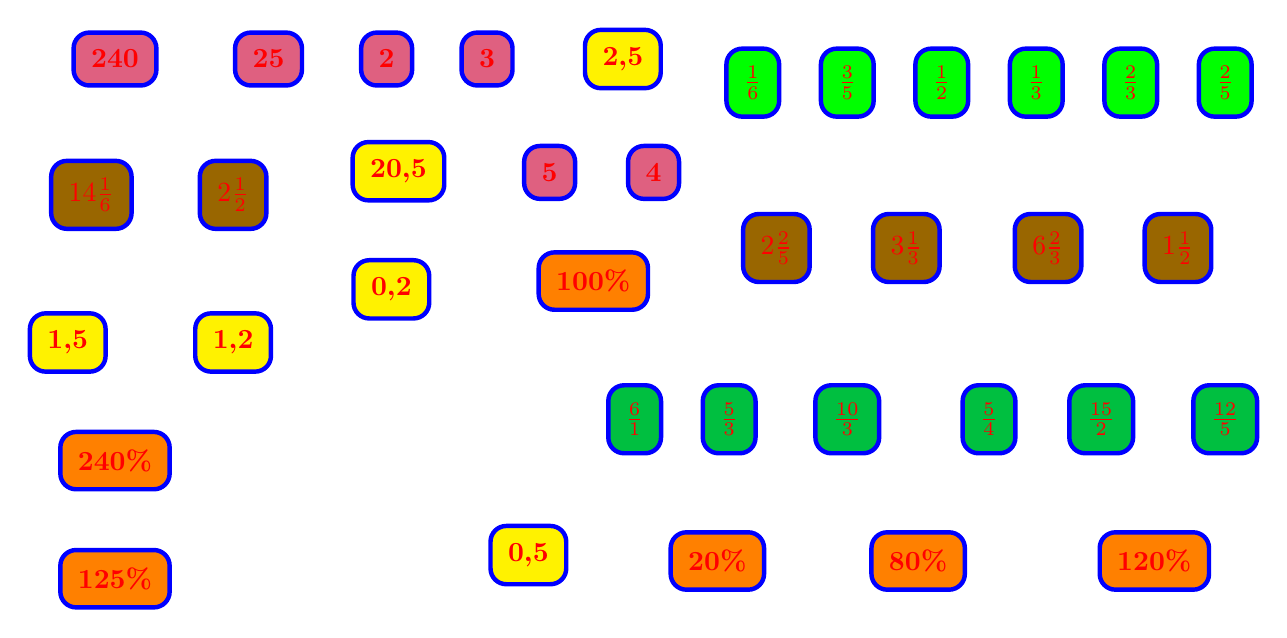
\begin{tikzpicture}[scale=1.5]
\node[red,draw=blue, rounded corners=.2cm, line width=0.5628571428571mm, fill=purple!50!pink] (leaf1) at  (0.0, 0.2)  {$\colorbox{purple!50!pink}{\textbf{240}}$};
\node[red,draw=blue, rounded corners=.2cm, line width=0.5628571428571mm, fill=purple!50!pink] (leaf2) at  (1.3, 0.2)  {$\colorbox{purple!50!pink}{\textbf{25}}$};
\node[red,draw=blue, rounded corners=.2cm, line width=0.5628571428571mm, fill=purple!50!pink] (leaf3) at  (2.3, 0.2)  {$\colorbox{purple!50!pink}{\textbf{2}}$};
\node[red,draw=blue, rounded corners=.2cm, line width=0.5628571428571mm, fill=purple!50!pink] (leaf4) at  (3.15, 0.2)  {$\colorbox{purple!50!pink}{\textbf{3}}$};
\node[red,draw=blue, rounded corners=.2cm, line width=0.5628571428571mm, fill=purple!50!pink] (leaf5) at  (4.56, -0.76)  {$\colorbox{purple!50!pink}{\textbf{4}}$};
\node[red,draw=blue, rounded corners=.2cm, line width=0.5628571428571mm, fill=purple!50!pink] (leaf6) at  (3.68, -0.76)  {$\colorbox{purple!50!pink}{\textbf{5}}$};
\node[red,draw=blue, rounded corners=.2cm, line width=0.5628571428571mm, fill=yellow] (leaf7) at  (2.4, -0.75)  {$\colorbox{yellow}{\textbf{20,5}}$};
\node[red,draw=blue, rounded corners=.2cm, line width=0.5628571428571mm, fill=yellow] (leaf8) at  (4.3, 0.2)  {$\colorbox{yellow}{\textbf{2,5}}$};
\node[red,draw=blue, rounded corners=.2cm, line width=0.5628571428571mm, fill=yellow] (leaf9) at  (-0.4, -2.2)  {$\colorbox{yellow}{\textbf{1,5}}$};
\node[red,draw=blue, rounded corners=.2cm, line width=0.5628571428571mm, fill=yellow] (leaf10) at  (1.0, -2.2)  {$\colorbox{yellow}{\textbf{1,2}}$};
\node[red,draw=blue, rounded corners=.2cm, line width=0.5628571428571mm, fill=yellow] (leaf11) at  (2.34, -1.75)  {$\colorbox{yellow}{\textbf{0,2}}$};
\node[red,draw=blue, rounded corners=.2cm, line width=0.5628571428571mm, fill=yellow] (leaf12) at  (3.5, -4.0)  {$\colorbox{yellow}{\textbf{0,5}}$};

\node[red,draw=blue, rounded corners=.2cm, line width=0.5628571428571mm, fill=green] (leaf1) at  (5.4, 0.0)  {$\colorbox{green}{\textbf{$\frac{1}{6}$}}$};
\node[red,draw=blue, rounded corners=.2cm, line width=0.5628571428571mm, fill=green] (leaf2) at  (6.2, 0.0)  {$\colorbox{green}{\textbf{$\frac{3}{5}$}}$};
\node[red,draw=blue, rounded corners=.2cm, line width=0.5628571428571mm, fill=green] (leaf3) at  (7.0, 0.0)  {$\colorbox{green}{$\frac{1}{2}$}$};
\node[red,draw=blue, rounded corners=.2cm, line width=0.5628571428571mm, fill=green] (leaf4) at  (7.8, 0.0)  {$\colorbox{green}{$\frac{1}{3}$}$};
\node[red,draw=blue, rounded corners=.2cm, line width=0.5628571428571mm, fill=green] (leaf5) at  (8.6, 0.0)  {$\colorbox{green}{$\frac{2}{3}$}$};
\node[red,draw=blue, rounded corners=.2cm, line width=0.5628571428571mm, fill=green] (leaf6) at  (9.4, 0.0)  {$\colorbox{green}{$\frac{2}{5}$}$};
\node[red,draw=blue, rounded corners=.2cm, line width=0.5628571428571mm, fill=red!60!green] (leaf7) at  (5.6, -1.4)  {$\colorbox{red!60!green}{\textbf{$2\frac{2}{5}$}}$};
\node[red,draw=blue, rounded corners=.2cm, line width=0.5628571428571mm, fill=red!60!green] (leaf8) at  (6.7, -1.4)  {$\colorbox{red!60!green}{\textbf{$3\frac{1}{3}$}}$};
\node[red,draw=blue, rounded corners=.2cm, line width=0.5628571428571mm, fill=red!60!green] (leaf9) at  (7.9, -1.4)  {$\colorbox{red!60!green}{$6\frac{2}{3}$}$};
\node[red,draw=blue, rounded corners=.2cm, line width=0.5628571428571mm, fill=red!60!green] (leaf10) at  (9.0,-1.4)  {$\colorbox{red!60!green}{$1\frac{1}{2}$}$};
\node[red,draw=blue, rounded corners=.2cm, line width=0.5628571428571mm, fill=red!60!green] (leaf11) at  (1.0, -0.95)  {$\colorbox{red!60!green}{$2\frac{1}{2}$}$};
\node[red,draw=blue, rounded corners=.2cm, line width=0.5628571428571mm, fill=red!60!green] (leaf12) at  (-0.2, -0.95)  {$\colorbox{red!60!green}{14$\frac{1}{6}$}$};

\node[red,draw=blue, rounded corners=.2cm, line width=0.5628571428571mm, fill=orange] (leaf1) at  (0.0, -3.2)  {$\colorbox{orange}{\textbf{240\%}}$};
\node[red,draw=blue, rounded corners=.2cm, line width=0.5628571428571mm, fill=orange] (leaf2) at  (0.0, -4.2)  {$\colorbox{orange}{\textbf{125\%}}$};
\node[red,draw=blue, rounded corners=.2cm, line width=0.5628571428571mm, fill=orange] (leaf3) at  (8.8, -4.05)  {$\colorbox{orange}{\textbf{120\%}}$};
\node[red,draw=blue, rounded corners=.2cm, line width=0.5628571428571mm, fill=orange] (leaf4) at  (6.8, -4.05)  {$\colorbox{orange}{\textbf{80\%}}$};
\node[red,draw=blue, rounded corners=.2cm, line width=0.5628571428571mm, fill=orange] (leaf5) at  (4.05, -1.68)  {$\colorbox{orange}{\textbf{100\%}}$};
\node[red,draw=blue, rounded corners=.2cm, line width=0.5628571428571mm, fill=orange] (leaf6) at  (5.1, -4.05)  {$\colorbox{orange}{\textbf{20\%}}$};
\node[red,draw=blue, rounded corners=.2cm, line width=0.5628571428571mm, fill=green!75!blue] (leaf7) at  (4.4, -2.85)  {$\colorbox{green!75!blue}{\textbf{$\frac{6}{1}$}}$};
\node[red,draw=blue, rounded corners=.2cm, line width=0.5628571428571mm, fill=green!75!blue] (leaf8) at  (5.2, -2.85)  {$\colorbox{green!75!blue}{\textbf{$\frac{5}{3}$}}$};
\node[red,draw=blue, rounded corners=.2cm, line width=0.5628571428571mm, fill=green!75!blue] (leaf9) at  (6.2, -2.85)  {$\colorbox{green!75!blue}{$\frac{10}{3}$}$};
\node[red,draw=blue, rounded corners=.2cm, line width=0.5628571428571mm, fill=green!75!blue] (leaf10) at  (7.4, -2.85)  {$\colorbox{green!75!blue}{$\frac{5}{4}$}$};
\node[red,draw=blue, rounded corners=.2cm, line width=0.5628571428571mm, fill=green!75!blue] (leaf11) at  (8.35, -2.85)  {$\colorbox{green!75!blue}{$\frac{15}{2}$}$};
\node[red,draw=blue, rounded corners=.2cm, line width=0.5628571428571mm, fill=green!75!blue] (leaf12) at  (9.4, -2.85)  {$\colorbox{green!75!blue}{$\frac{12}{5}$}$};
\end{tikzpicture}}

Iš krūvos išsirinksime dvi vienodų arba skirtingų spalvų korteles. Prieš išsirenkant korteles siūlau pamėginti atlikti treniruotę, kad įsitikintum, jog tavo žinios atlikti tolimesniems uždaviniams yra pakankamos. 
Klausimams 2 - 4 atsakyti mokinys gali pasinaudoti patarimais:
{\small
\begin{itemize}
\item pamėgink pasirinkti vienodas spalvas ir pastebėti dėsningumą.
\item pamėgink pasirinkti tas spalvas, su kuriomis skaičiavimą įveiki.
\item su pradžioje pasirinktomis kortelėmis pakartok 2 pratimą.
\item pamėgink abejose kortelėse esančius skaičius nusibraižyti sąsiuvinyje naudodamas geometrines figūras.
\item jei šis klausimas vis dar per sunkus, prašyk mokytojo pagalbos.
\end{itemize}}
\textit{Pastaba: prižiūrinčiam mokytojui galima užsivesti suvestinę, kurioje būtų fiksuojami mokinio gebėjimai atlikti 2 - 4 užduotis su visomis 18 spalvų porų}

Siūlomi pratimai:
\begin{enumerate}
\item Atsitiktinai ištrauk dvi korteles:
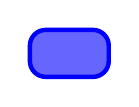
\begin{tikzpicture}[scale=1.5, baseline=-0.7ex]\node[red,draw=blue, rounded corners=.2cm, line width=0.5628571428571mm, fill=white!40!blue] (leaf1) at  (0.0, 0.0)  {$\colorbox{white!40!blue}{\phantom{xxx}}$};\end{tikzpicture}
ir
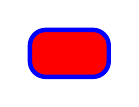
\begin{tikzpicture}[scale=1.5, baseline=-0.7ex]\node[red,draw=blue, rounded corners=.2cm, line width=0.5628571428571mm, fill=red] (leaf1) at  (0.0, 0.0)  {$\colorbox{red}{\phantom{xxx}}$};\end{tikzpicture}. Jų spalvos bus kitokios, bet jas taip pažymėjome norėdami trumpai įvardinti pirmą ir antrą korteles. Perskaityk, kas parašyta kortelėse. Pavyzdžiui 14,8 yra keturiolika ir 8 dešimtosios arba $\frac{2}{5}$ yra dvi penktosios.
\item Įvardyk abejose kortelėse esančių skaičių rūšis. Ar gali kortelės 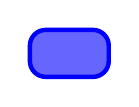
\begin{tikzpicture}[scale=1.5, baseline=-0.7ex]\node[red,draw=blue, rounded corners=.2cm, line width=0.5628571428571mm, fill=white!40!blue] (leaf1) at  (0.0, 0.0)  {$\colorbox{white!40!blue}{\phantom{xxx}}$};\end{tikzpicture} skaičiaus rūšį paversti į tokią rūšį, kuri yra kortelėje 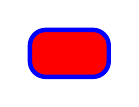
\begin{tikzpicture}[scale=1.5, baseline=-0.7ex]\node[red,draw=blue, rounded corners=.2cm, line width=0.5628571428571mm, fill=red] (leaf1) at  (0.0, 0.0)  {$\colorbox{red}{\phantom{xxx}}$};\end{tikzpicture}? Ar gali kortelės 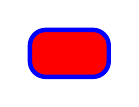
\begin{tikzpicture}[scale=1.5, baseline=-0.7ex]\node[red,draw=blue, rounded corners=.2cm, line width=0.5628571428571mm, fill=red] (leaf1) at  (0.0, 0.0)  {$\colorbox{red}{\phantom{xxx}}$};\end{tikzpicture} skaičiaus rūšį paversti į tokią rūšį, kuri yra kortelėje 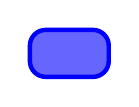
\begin{tikzpicture}[scale=1.5, baseline=-0.7ex]\node[red,draw=blue, rounded corners=.2cm, line width=0.5628571428571mm, fill=white!40!blue] (leaf1) at  (0.0, 0.0)  {$\colorbox{white!40!blue}{\phantom{xxx}}$};\end{tikzpicture}?
\item Kiek skaičiaus, kurio vertė yra 
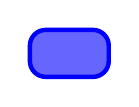
\begin{tikzpicture}[scale=1.5, baseline=-0.7ex]\node[red,draw=blue, rounded corners=.2cm, line width=0.5628571428571mm, fill=white!40!blue] (leaf1) at  (0.0, 0.0)  {$\colorbox{white!40!blue}{\phantom{xxx}}$};\end{tikzpicture}
sudaro skaičiaus, kurio vertė yra
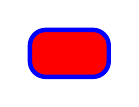
\begin{tikzpicture}[scale=1.5, baseline=-0.7ex]\node[red,draw=blue, rounded corners=.2cm, line width=0.5628571428571mm, fill=red] (leaf1) at  (0.0, 0.0)  {$\colorbox{red}{\phantom{xxx}}$};\end{tikzpicture}? 
\item a) \textit{(Atsakyti tada, kai antroje kortelėje ištrauktas skaičius nėra sveikasis)}. Skaičius, kurio vertė yra 
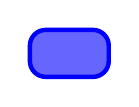
\begin{tikzpicture}[scale=1.5, baseline=-0.7ex]\node[red,draw=blue, rounded corners=.2cm, line width=0.5628571428571mm, fill=white!40!blue] (leaf1) at  (0.0, 0.0)  {$\colorbox{white!40!blue}{\phantom{xxx}}$};\end{tikzpicture} sudaro 
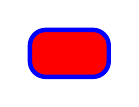
\begin{tikzpicture}[scale=1.5, baseline=-0.7ex]\node[red,draw=blue, rounded corners=.2cm, line width=0.5628571428571mm, fill=red] (leaf1) at  (0.0, 0.0)  {$\colorbox{red}{\phantom{xxx}}$};\end{tikzpicture} dalies (dalį) reikiamos vertės. Kokia yra reikiama vertė?

 b) \textit{(Atsakyti tada, kai antroje kortelėje ištrauktas skaičius yra sveikasis)}. Skaičius, kurio vertė yra 
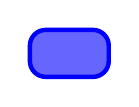
\begin{tikzpicture}[scale=1.5, baseline=-0.7ex]\node[red,draw=blue, rounded corners=.2cm, line width=0.5628571428571mm, fill=white!40!blue] (leaf1) at  (0.0, 0.0)  {$\colorbox{white!40!blue}{\phantom{xxx}}$};\end{tikzpicture} yra
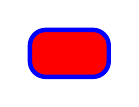
\begin{tikzpicture}[scale=1.5, baseline=-0.7ex]\node[red,draw=blue, rounded corners=.2cm, line width=0.5628571428571mm, fill=red] (leaf1) at  (0.0, 0.0)  {$\colorbox{red}{\phantom{xxx}}$};\end{tikzpicture} kartų (kartus) daugiau už reikiamą vertę. Kokia yra reikiama vertė?
\item Kiek dvyliktųjų sudaro skaičius $\frac{1}{3}$ ir $\frac{1}{4}$? Kaip šie rezultatai susiję su suma $\frac{1}{3}+\frac{1}{4}$? Panašiai samprotaudami apskaičiuokite veiksmus $\frac{2}{3}+\frac{1}{4}$, $\frac{3}{4}+\frac{4}{5}$, $\frac{1}{5}-\frac{1}{7}$, $\frac{1}{3}-\frac{1}{6}$, $\frac{1}{3}+\frac{1}{6}$.
\end{enumerate}
\end{mybox}

\begin{mybox}{Mokomės hipotetiškai mąstyti$\text{,}$ tiksliai formuluoti teiginius$\text{,}$ suprasti ir atskirti sąvokas}
Ant stalo turime daug žodžių, apibūdinančių įvairias savybes. 

\begin{tikzpicture}[scale=1.5]
\node[red,draw=blue, rounded corners=.2cm, line width=0.5628571428571mm, fill=yellow] (leaf1) at  (0,0)  {$\colorbox{yellow}{\textbf{nuobodumas}}$}; %nuobodėja, įdomėja
\node[red,draw=blue, rounded corners=.2cm, line width=0.5628571428571mm, fill=yellow] (leaf2) at  (0,-0.5)  {$\colorbox{yellow}{\textbf{gudrumas}}$}; %gudrėja, kvailėja
\node[red,draw=blue, rounded corners=.2cm, line width=0.5628571428571mm, fill=yellow] (leaf3) at  (0,-1)  {$\colorbox{yellow}{\textbf{šiurkštumas}}$}; %šiurkštėja, minkštėja, švelnėja
\node[red,draw=blue, rounded corners=.2cm, line width=0.5628571428571mm, fill=yellow] (leaf4) at  (0, -1.5)  {$\colorbox{yellow}{\textbf{konkretumas}}$}; %konkretėja, abstraktėja
\node[red,draw=blue, rounded corners=.2cm, line width=0.5628571428571mm, fill=yellow] (leaf5) at  (0, -2)  {$\colorbox{yellow}{\textbf{tvirtumas}}$}; %tvirtėja, silpsta
\node[red,draw=blue, rounded corners=.2cm, line width=0.5628571428571mm, fill=yellow] (leaf6) at  (0, -2.5)  {$\colorbox{yellow}{\textbf{svoris}}$}; %sunkėja, lengvėja
\node[red,draw=blue, rounded corners=.2cm, line width=0.5628571428571mm, fill=yellow] (leaf7) at  (0, -3)  {$\colorbox{yellow}{\textbf{dydis}}$}; %didėja, mažėja
\node[red,draw=blue, rounded corners=.2cm, line width=0.5628571428571mm, fill=yellow] (leaf8) at  (0, -3.5)  {$\colorbox{yellow}{\textbf{plotas}}$};  %didėja, mažėja
\node[red,draw=blue, rounded corners=.2cm, line width=0.5628571428571mm, fill=yellow] (leaf9) at  (0, -4)  {$\colorbox{yellow}{\textbf{greitis}}$}; %greitėja, lėtėja
\node[red,draw=blue, rounded corners=.2cm, line width=0.5628571428571mm, fill=yellow] (leaf10) at  (0, -4.5)  {$\colorbox{yellow}{\textbf{tirštumas}}$}; %tirštėja, skystėja
\node[red,draw=blue, rounded corners=.2cm, line width=0.5628571428571mm, fill=yellow] (leaf11) at  (0, -5)  {$\colorbox{yellow}{\textbf{gylis}}$}; %gilėja, seklėja
\node[red,draw=blue, rounded corners=.2cm, line width=0.5628571428571mm, fill=yellow] (leaf12) at  (0, -5.5)  {$\colorbox{yellow}{\textbf{tankumas}}$}; %tankėja, retėja
\node[red,draw=blue, rounded corners=.2cm, line width=0.5628571428571mm, fill=red] (leaf13) at  (0, -6)  {$\colorbox{red}{\textbf{trukmė}}$}; %tankėja, retėja
\node[red,draw=blue, rounded corners=.2cm, line width=0.5628571428571mm, fill=red] (leaf14) at  (0, -6.5)  {$\colorbox{red}{\textbf{atkarpa}}$}; %tankėja, retėja
\node[red,draw=blue, rounded corners=.2cm, line width=0.5628571428571mm, fill=red] (leaf15) at  (0, -7)  {$\colorbox{red}{\textbf{sąryšis}}$}; %tankėja, retėja
\node[red,draw=blue, rounded corners=.2cm, line width=0.5628571428571mm, fill=red] (leaf16) at  (0, -7.5)  {$\colorbox{red}{\textbf{operacija}}$}; %tankėja, retėja

\node[red,draw=blue, rounded corners=.2cm, line width=0.5628571428571mm, fill=yellow] (leaf1) at  (1.5, 0)  {$\colorbox{yellow}{\textbf{masė}}$}; %sunkėja, lengvėja
\node[red,draw=blue, rounded corners=.2cm, line width=0.5628571428571mm, fill=yellow] (leaf2) at  (1.5, -0.5)  {$\colorbox{yellow}{\textbf{dažnumas}}$}; %dažnėja, retėja
\node[red,draw=blue, rounded corners=.2cm, line width=0.5628571428571mm, fill=yellow] (leaf3) at  (1.5, -1)  {$\colorbox{yellow}{\textbf{garsas}}$}; %garsėja, tyla
\node[red,draw=blue, rounded corners=.2cm, line width=0.5628571428571mm, fill=yellow] (leaf4) at  (1.5, -1.5)  {$\colorbox{yellow}{\textbf{plotis}}$}; %darbštėja, tingėja
\node[red,draw=blue, rounded corners=.2cm, line width=0.5628571428571mm, fill=yellow] (leaf5) at  (1.5, -2)  {$\colorbox{yellow}{\textbf{ryškumas}}$}; %ryškėja, blanksta, blunka
\node[red,draw=blue, rounded corners=.2cm, line width=0.5628571428571mm, fill=yellow] (leaf6) at  (1.5, -2.5)  {$\colorbox{yellow}{\textbf{darbštumas}}$}; %platėja, siaurėja, traukiasi
\node[red,draw=blue, rounded corners=.2cm, line width=0.5628571428571mm, fill=yellow] (leaf7) at  (1.5, -3)  {$\colorbox{yellow}{\textbf{intensyvumas}}$}; %intensyvėja, slopsta
\node[red,draw=blue, rounded corners=.2cm, line width=0.5628571428571mm, fill=yellow] (leaf8) at  (1.5, -3.5)  {$\colorbox{yellow}{\textbf{kietumas}}$}; %kietėja, skystėja
\node[red,draw=blue, rounded corners=.2cm, line width=0.5628571428571mm, fill=yellow] (leaf9) at  (1.5, -4)  {$\colorbox{yellow}{\textbf{kaina}}$}; %brangsta, pinga
\node[red,draw=blue, rounded corners=.2cm, line width=0.5628571428571mm, fill=yellow] (leaf10) at  (1.5, -4.5)  {$\colorbox{yellow}{\textbf{lygis}}$}; %gerėja, blogėja, tvinsta, senka
\node[red,draw=blue, rounded corners=.2cm, line width=0.5628571428571mm, fill=yellow] (leaf11) at  (1.5, -5.0)  {$\colorbox{yellow}{\textbf{įvairovė}}$}; %įvairėja, panašėja, vienodėja
\node[red,draw=blue, rounded corners=.2cm, line width=0.5628571428571mm, fill=yellow] (leaf12) at  (1.5, -5.5)  {$\colorbox{yellow}{\textbf{nuotolis}}$}; %tolsta, artėja
\node[red,draw=blue, rounded corners=.2cm, line width=0.5628571428571mm, fill=red] (leaf13) at  (1.5, -6.0)  {$\colorbox{red}{\textbf{matmuo}}$}; %tankėja, retėja
\node[red,draw=blue, rounded corners=.2cm, line width=0.5628571428571mm, fill=red] (leaf14) at  (1.5, -6.5)  {$\colorbox{red}{\textbf{tiesė}}$}; %tankėja, retėja
\node[red,draw=blue, rounded corners=.2cm, line width=0.5628571428571mm, fill=red] (leaf15) at  (1.5, -7)  {$\colorbox{red}{\textbf{figūra}}$}; %tankėja, retėja
\node[red,draw=blue, rounded corners=.2cm, line width=0.5628571428571mm, fill=red] (leaf16) at  (1.5, -7.5)  {$\colorbox{red}{\textbf{narys}}$}; %tankėja, retėja

\node[red,draw=blue, rounded corners=.2cm, line width=0.5628571428571mm, fill=yellow] (leaf1) at  (3, 0)  {$\colorbox{yellow}{\textbf{drėgmė}}$}; %drėgsta, sausėja
\node[red,draw=blue, rounded corners=.2cm, line width=0.5628571428571mm, fill=yellow] (leaf2) at  (3, -0.5)  {$\colorbox{yellow}{\textbf{atlaidumas}}$}; %atlaidėja, griežtėja
\node[red,draw=blue, rounded corners=.2cm, line width=0.5628571428571mm, fill=yellow] (leaf3) at  (3, -1)  {$\colorbox{yellow}{\textbf{temperatūra}}$}; %šyla, karštėja, kaista, šąla
\node[red,draw=blue, rounded corners=.2cm, line width=0.5628571428571mm, fill=yellow] (leaf4) at  (3, -1.5)  {$\colorbox{yellow}{\textbf{kokybė}}$}; %kokybiškėja, gerėja
\node[red,draw=blue, rounded corners=.2cm, line width=0.5628571428571mm, fill=yellow] (leaf5) at  (3, -2)  {$\colorbox{yellow}{\textbf{storis}}$}; %storėja, plonėja, traukiasi
\node[red,draw=blue, rounded corners=.2cm, line width=0.5628571428571mm, fill=yellow] (leaf6) at  (3, -2.5)  {$\colorbox{yellow}{\textbf{talpa}}$}; %turtingėja, skurdėja
\node[red,draw=blue, rounded corners=.2cm, line width=0.5628571428571mm, fill=yellow] (leaf7) at  (3, -3)  {$\colorbox{yellow}{\textbf{sparta}}$}; %spartėja, lėtėja
\node[red,draw=blue, rounded corners=.2cm, line width=0.5628571428571mm, fill=yellow] (leaf8) at  (3, -3.5)  {$\colorbox{yellow}{\textbf{stiprumas}}$}; %stiprėja, silpnėja
\node[red,draw=blue, rounded corners=.2cm, line width=0.5628571428571mm, fill=yellow] (leaf9) at  (3, -4)  {$\colorbox{yellow}{\textbf{šviesumas}}$}; %šviesėja, tamsėja
\node[red,draw=blue, rounded corners=.2cm, line width=0.5628571428571mm, fill=yellow] (leaf10) at  (3, -4.5)  {$\colorbox{yellow}{\textbf{turtingumas}}$}; %didėja, mažėja
\node[red,draw=blue, rounded corners=.2cm, line width=0.5628571428571mm, fill=yellow] (leaf11) at  (3, -5)  {$\colorbox{yellow}{\textbf{ilgis}}$}; %ilgėja, trumpėja
\node[red,draw=blue, rounded corners=.2cm, line width=0.5628571428571mm, fill=yellow] (leaf12) at  (3, -5.5)  {$\colorbox{yellow}{\textbf{aukštis}}$}; %aukštėja, žemėja
\node[red,draw=blue, rounded corners=.2cm, line width=0.5628571428571mm, fill=red] (leaf13) at  (3, -6.0)  {$\colorbox{red}{\textbf{dydis}}$}; %tankėja, retėja
\node[red,draw=blue, rounded corners=.2cm, line width=0.5628571428571mm, fill=red] (leaf14) at  (3, -6.5)  {$\colorbox{red}{\textbf{reikšmė}}$}; %tankėja, retėja
\node[red,draw=blue, rounded corners=.2cm, line width=0.5628571428571mm, fill=red] (leaf15) at  (3, -7)  {$\colorbox{red}{\textbf{kiekis}}$}; %tankėja, retėja
\node[red,draw=blue, rounded corners=.2cm, line width=0.5628571428571mm, fill=red] (leaf16) at  (3, -7.5)  {$\colorbox{red}{\textbf{objektas}}$}; %tankėja, retėja


%talpa, temperatūra, lygis, kaina, plotas, svoris, masė

\node[red,draw=blue, rounded corners=.2cm, line width=0.5628571428571mm, fill=orange] (leaf1) at  (4.5, 0)  {$\colorbox{orange}{\textbf{kraštinė}}$};
\node[red,draw=blue, rounded corners=.2cm, line width=0.5628571428571mm, fill=orange] (leaf2) at  (4.5, -0.5)  {$\colorbox{orange}{\textbf{santykis}}$};
\node[red,draw=blue, rounded corners=.2cm, line width=0.5628571428571mm, fill=orange] (leaf3) at  (4.5, -1)  {$\colorbox{orange}{\textbf{atimtis}}$};
\node[red,draw=blue, rounded corners=.2cm, line width=0.5628571428571mm, fill=orange] (leaf4) at  (4.5, -1.5)  {$\colorbox{orange}{\textbf{atstumas}}$};
\node[red,draw=blue, rounded corners=.2cm, line width=0.5628571428571mm, fill=orange] (leaf5) at  (4.5, -2)  {$\colorbox{orange}{\textbf{greitis}}$};
\node[red,draw=blue, rounded corners=.2cm, line width=0.5628571428571mm, fill=orange] (leaf6) at  (4.5, -2.5)  {$\colorbox{orange}{\textbf{vertė}}$};
\node[red,draw=blue, rounded corners=.2cm, line width=0.5628571428571mm, fill=orange] (leaf7) at  (4.5, -3)  {$\colorbox{orange}{\textbf{kiekis}}$};
\node[red,draw=blue, rounded corners=.2cm, line width=0.5628571428571mm, fill=orange] (leaf8) at  (4.5, -3.5)  {$\colorbox{orange}{\textbf{dydis}}$};
\node[red,draw=blue, rounded corners=.2cm, line width=0.5628571428571mm, fill=orange] (leaf9) at  (4.5, -4)  {$\colorbox{orange}{\textbf{statmuo}}$};
\node[red,draw=blue, rounded corners=.2cm, line width=0.5628571428571mm, fill=orange] (leaf10) at  (4.5, -4.5)  {$\colorbox{orange}{\textbf{kvadratas}}$};
\node[red,draw=blue, rounded corners=.2cm, line width=0.5628571428571mm, fill=orange] (leaf11) at  (4.5, -5)  {$\colorbox{orange}{\textbf{trikampis}}$};
\node[red,draw=blue, rounded corners=.2cm, line width=0.5628571428571mm, fill=orange] (leaf12) at  (4.5, -5.5)  {$\colorbox{orange}{\textbf{stačiakampis}}$};
\node[red,draw=blue, rounded corners=.2cm, line width=0.5628571428571mm, fill=orange] (leaf13) at  (4.5, -6)  {$\colorbox{orange}{\textbf{šaknis}}$};
\node[red,draw=blue, rounded corners=.2cm, line width=0.5628571428571mm, fill=red] (leaf14) at  (4.5, -6.5)  {$\colorbox{red}{\textbf{skaičius}}$}; %tankėja, retėja
\node[red,draw=blue, rounded corners=.2cm, line width=0.5628571428571mm, fill=red] (leaf15) at  (4.5, -7)  {$\colorbox{red}{\textbf{kelias}}$}; %tankėja, retėja
\node[red,draw=blue, rounded corners=.2cm, line width=0.5628571428571mm, fill=red] (leaf16) at  (4.5, -7.5)  {$\colorbox{red}{\textbf{lygybė}}$}; %tankėja, retėja

\node[red,draw=blue, rounded corners=.2cm, line width=0.5628571428571mm, fill=orange] (leaf1) at  (6, 0)  {$\colorbox{orange}{\textbf{trapecija}}$};
\node[red,draw=blue, rounded corners=.2cm, line width=0.5628571428571mm, fill=orange] (leaf2) at  (6, -0.5)  {$\colorbox{orange}{\textbf{daugyba}}$};
\node[red,draw=blue, rounded corners=.2cm, line width=0.5628571428571mm, fill=orange] (leaf3) at  (6,-1)  {$\colorbox{orange}{\textbf{perimetras}}$};
\node[red,draw=blue, rounded corners=.2cm, line width=0.5628571428571mm, fill=orange] (leaf4) at  (6,-1.5)  {$\colorbox{orange}{\textbf{plotas}}$};
\node[red,draw=blue, rounded corners=.2cm, line width=0.5628571428571mm, fill=orange] (leaf5) at  (6,-2)  {$\colorbox{orange}{\textbf{kampas}}$};
\node[red,draw=blue, rounded corners=.2cm, line width=0.5628571428571mm, fill=orange] (leaf6) at  (6,-2.5)  {$\colorbox{orange}{\textbf{sudėtis}}$};
\node[red,draw=blue, rounded corners=.2cm, line width=0.5628571428571mm, fill=orange] (leaf7) at  (6,-3)  {$\colorbox{orange}{\textbf{spindulys}}$};
\node[red,draw=blue, rounded corners=.2cm, line width=0.5628571428571mm, fill=orange] (leaf8) at  (6, -3.5)  {$\colorbox{orange}{\textbf{taškas}}$};
\node[red,draw=blue, rounded corners=.2cm, line width=0.5628571428571mm, fill=orange] (leaf9) at  (6, -4)  {$\colorbox{orange}{\textbf{tiesė}}$};
\node[red,draw=blue, rounded corners=.2cm, line width=0.5628571428571mm, fill=orange] (leaf10) at  (6, -4.5)  {$\colorbox{orange}{\textbf{atkarpa}}$};
\node[red,draw=blue, rounded corners=.2cm, line width=0.5628571428571mm, fill=orange] (leaf11) at  (6,-5)  {$\colorbox{orange}{\textbf{rombas}}$};
\node[red,draw=blue, rounded corners=.2cm, line width=0.5628571428571mm, fill=orange] (leaf12) at  (6,-5.5)  {$\colorbox{orange}{\textbf{dalyba}}$};
\node[red,draw=blue, rounded corners=.2cm, line width=0.5628571428571mm, fill=orange] (leaf13) at  (6, -6)  {$\colorbox{orange}{\textbf{kintamasis}}$};
\node[red,draw=blue, rounded corners=.2cm, line width=0.5628571428571mm, fill=orange] (leaf14) at  (6, -6.5)  {$\colorbox{orange}{\textbf{nežinomasis}}$}; %tankėja, retėja
\node[red,draw=blue, rounded corners=.2cm, line width=0.5628571428571mm, fill=red] (leaf15) at  (6, -7)  {$\colorbox{red}{\textbf{kiekis}}$}; %tankėja, retėja
\node[red,draw=blue, rounded corners=.2cm, line width=0.5628571428571mm, fill=red] (leaf16) at  (6, -7.5)  {$\colorbox{red}{\textbf{simbolis}}$}; %tankėja, retėja

\node[red,draw=blue, rounded corners=.2cm, line width=0.5628571428571mm, fill=orange] (leaf1) at  (7.5,0)  {$\colorbox{orange}{\textbf{atėminys}}$};
\node[red,draw=blue, rounded corners=.2cm, line width=0.5628571428571mm, fill=orange] (leaf2) at  (7.5, -0.5)  {$\colorbox{orange}{\textbf{skirtumas}}$};
\node[red,draw=blue, rounded corners=.2cm, line width=0.5628571428571mm, fill=orange] (leaf3) at  (7.5,-1)  {$\colorbox{orange}{\textbf{daugiklis}}$};
\node[red,draw=blue, rounded corners=.2cm, line width=0.5628571428571mm, fill=orange] (leaf4) at  (7.5,-1.5)  {$\colorbox{orange}{\textbf{dauginys}}$};
\node[red,draw=blue, rounded corners=.2cm, line width=0.5628571428571mm, fill=orange] (leaf5) at  (7.5, -2)  {$\colorbox{orange}{\textbf{sandauga}}$};
\node[red,draw=blue, rounded corners=.2cm, line width=0.5628571428571mm, fill=orange] (leaf6) at  (7.5, -2.5)  {$\colorbox{orange}{\textbf{dalinys}}$};
\node[red,draw=blue, rounded corners=.2cm, line width=0.5628571428571mm, fill=orange] (leaf7) at  (7.5, -3)  {$\colorbox{orange}{\textbf{daliklis}}$};
\node[red,draw=blue, rounded corners=.2cm, line width=0.5628571428571mm, fill=orange] (leaf8) at  (7.5, -3.5)  {$\colorbox{orange}{\textbf{dalmuo}}$};
\node[red,draw=blue, rounded corners=.2cm, line width=0.5628571428571mm, fill=orange] (leaf9) at  (7.5, -4)  {$\colorbox{orange}{\textbf{dėmuo}}$};
\node[red,draw=blue, rounded corners=.2cm, line width=0.5628571428571mm, fill=orange] (leaf10) at  (7.5, -4.5)  {$\colorbox{orange}{\textbf{suma}}$};
\node[red,draw=blue, rounded corners=.2cm, line width=0.5628571428571mm, fill=orange] (leaf11) at  (7.5, -5)  {$\colorbox{orange}{\textbf{greitis}}$};
\node[red,draw=blue, rounded corners=.2cm, line width=0.5628571428571mm, fill=orange] (leaf12) at  (7.5, -5.5)  {$\colorbox{orange}{\textbf{dalyba}}$};
\node[red,draw=blue, rounded corners=.2cm, line width=0.5628571428571mm, fill=orange] (leaf13) at  (7.5, -6)  {$\colorbox{orange}{\textbf{laipsnis}}$};
\node[red,draw=blue, rounded corners=.2cm, line width=0.5628571428571mm, fill=red] (leaf14) at  (7.5, -6.5)  {$\colorbox{red}{\textbf{aibė}}$};
\node[red,draw=blue, rounded corners=.2cm, line width=0.5628571428571mm, fill=orange] (leaf15) at  (7.5, -7)  {$\colorbox{orange}{\textbf{turinys}}$}; %tankėja, retėja
\node[red,draw=blue, rounded corners=.2cm, line width=0.5628571428571mm, fill=red] (leaf16) at  (7.5, -7.5)  {$\colorbox{red}{\textbf{rezultatas}}$}; %tankėja, retėja

\node[red,draw=blue, rounded corners=.2cm, line width=0.5628571428571mm, fill=green] (leaf1) at  (9,0)  {$\colorbox{green}{\textbf{didėja}}$};
\node[red,draw=blue, rounded corners=.2cm, line width=0.5628571428571mm, fill=green] (leaf2) at  (9, -0.5)  {$\colorbox{green}{\textbf{kyla}}$};
\node[red,draw=blue, rounded corners=.2cm, line width=0.5628571428571mm, fill=green] (leaf3) at  (9,-1)  {$\colorbox{green}{\textbf{auga}}$};
\node[red,draw=blue, rounded corners=.2cm, line width=0.5628571428571mm, fill=green!70!blue] (leaf4) at  (9,-1.5)  {$\colorbox{green!70!blue}{\textbf{mažėja}}$};
\node[red,draw=blue, rounded corners=.2cm, line width=0.5628571428571mm, fill=green!70!blue] (leaf5) at  (9, -2)  {$\colorbox{green!70!blue}{\textbf{leidžiasi}}$};
\node[red,draw=blue, rounded corners=.2cm, line width=0.5628571428571mm, fill=green!70!blue] (leaf6) at  (9, -2.5)  {$\colorbox{green!70!blue}{\textbf{krenta}}$};
\node[red,draw=blue, rounded corners=.2cm, line width=0.5628571428571mm, fill=brown] (leaf7) at  (9, -3)  {$\colorbox{brown}{\textbf{didelis/ -ė}}$};
\node[red,draw=blue, rounded corners=.2cm, line width=0.5628571428571mm, fill=brown] (leaf8) at  (9, -3.5)  {$\colorbox{brown}{\textbf{aukštas/ -a}}$};
\node[red,draw=blue, rounded corners=.2cm, line width=0.5628571428571mm, fill=brown] (leaf9) at  (9, -4)  {$\colorbox{brown}{\textbf{pakilęs/ -us}}$};
\node[red,draw=blue, rounded corners=.2cm, line width=0.5628571428571mm, fill=brown] (leaf10) at  (9, -4.5)  {$\colorbox{brown}{\textbf{išaugęs/ -us}}$};
\node[red,draw=blue, rounded corners=.2cm, line width=0.5628571428571mm, fill=green!30!red] (leaf11) at  (9, -5)  {$\colorbox{green!30!red}{\textbf{mažas/ -a}}$};
\node[red,draw=blue, rounded corners=.2cm, line width=0.5628571428571mm, fill=green!30!red] (leaf12) at  (9, -5.5)  {$\colorbox{green!30!red}{\textbf{žemas/ -a}}$};
\node[red,draw=blue, rounded corners=.2cm, line width=0.5628571428571mm, fill=green!30!red] (leaf13) at  (9, -6)  {$\colorbox{green!30!red}{\textbf{nusileidęs/ -a}}$};
\node[red,draw=blue, rounded corners=.2cm, line width=0.5628571428571mm, fill=green!30!red] (leaf14) at  (9, -6.5)  {$\colorbox{green!30!red}{\textbf{nukritęs/ -us}}$};
\node[red,draw=blue, rounded corners=.2cm, line width=0.5628571428571mm, fill=orange] (leaf15) at  (9, -7)  {$\colorbox{orange}{\textbf{daugiakampis}}$}; %tankėja, retėja
\node[red,draw=blue, rounded corners=.2cm, line width=0.5628571428571mm, fill=orange] (leaf16) at  (9, -7.5)  {$\colorbox{orange}{\textbf{pagrindas}}$}; %tankėja, retėja
\end{tikzpicture}

Kiekviename pratime atsitiktinai reikės sugalvoti sudėtinį sakinį, susidedantį iš dviejų dėmenų, prasidedančių \textbf{\textit{jei}} ir \textbf{\textit{tai}}. Siūlomi pratimai:

\begin{enumerate}
\item Atsitiktinai traukiame kortelę \DrawCard{\phantom{xxx}}{yellow}. Pagrindiniame dėmenyje yra iš kortelių sudarytas žodžių junginys, į kurį įeina šios kortelės žodis, o šalutinis dėmuo yra pagrindiniam dėmeniui sinonimiškas teiginys. Atlikdamas atskiras pratimo dalis stenkis, kad sakiniai būtų logiški. 

\begin{itemize}
\item Junginys sudarytas iš kortelių \DrawCard{\phantom{xxx}}{yellow} ir \DrawCard{\phantom{xxx}}{green} žodžių:

\textit{Jei oro temperatūra kyla, tai oras šyla.}
\textit{Jei patiekalų įvairovė didėja, tai patiekalai įvairėja.}
\item Junginys sudarytas iš kortelių \DrawCard{\phantom{xxx}}{yellow} ir \DrawCard{\phantom{xxx}}{green!70!blue} žodžių:

\textit{Jei oro temperatūra krenta, tai oras šąla.}

\textit{Jei patiekalų įvairovė mažėja, tai $\bcancel{\cancel{\text{\textit{patiekalai panašėja}}}}$ patiekalų mažėja.}

\item Junginys sudarytas iš kortelių \DrawCard{\phantom{xxx}}{yellow} ir \DrawCard{\phantom{xxx}}{brown} žodžių:

\textit{Jei oro temperatūra aukšta, tai oras šiltas.}
\textit{Jei patiekalų įvairovė didelė, tai patiekalai įvairūs.}
\item Junginys sudarytas iš kortelių \DrawCard{\phantom{xxx}}{yellow} ir \DrawCard{\phantom{xxx}}{green!30!red} žodžių:

\textit{Jei oro temperatūra žema, tai oras vėsus.}

\textit{Jei patiekalų įvairovė maža, tai $\bcancel{\cancel{\text{\textit{patiekalai panašūs}}}}$ patiekalų nedaug.}
\end{itemize}
\item Atsitiktinai traukiame kortelę \DrawCard{\phantom{xxx}}{yellow}. Sugalvok sakinį, kuriame atsispindi \textit{\textbf{loginė išvada}}: pagrindiniame sakinio dėmenyje yra kortelės \DrawCard{\phantom{xxx}}{yellow} žodis, o šalutiniame dėmenyje yra kitos kortelės \DrawCard{\phantom{xxx}}{yellow}, kurią gali pasirinkti pats, žodis.

\textit{Jei oro temperatūra žema, tai kaina už šildymą aukšta.}

\textit{Jei prekių kaina kyla, tai piniginės storis mažėja.}
\end{enumerate}
\end{mybox}

\begin{mybox}{Mokomės suprasti$\text{,}$ skirti ir vartoti matematines sąvokas$\text{,}$ teiginius ir jų išvadas}
\begin{enumerate}\addtocounter{enumi}{2}
\item Atvirkštinis teiginys - tai teiginys, kuriame sakinio dalis, apibūdinanti priežastį, yra apkeista vietomis su sakinio dalimi, apibūdinančia pasekmę. 

Teiginiui \textit{jei prekių kaina kyla, tai piniginės storis mažėja} atvirkštinis teiginys būtų: \textit{jei piniginės storis mažėja, tai prekių kaina kyla}. 

Kiekvienam ankstesnio pratimo teiginiui sugalvok atvirkštinį teiginį.

\item \textbf{\textit{Gudresniesiems.}} Kurie iš ankstesniame pratimų sugalvotų teiginių yra teisingi, kurie neteisingi? Paaiškink kodėl.

Teiginys \textit{jei piniginės storis mažėja, tai prekių kaina kyla} ne visada galioja. Teiginys neteisingas, kai piniginės storis mažėja, tada, kai perkama daugiau prekių, nors prekių kaina ir nekyla.

\item \textbf{\textit{Gudresniesiems.}} Trečio pratimo sakinius, kuriems atvirkštiniai teiginiai taip pat teisingi, suformuluok jungdamas du sakinio dėmenis žodžių junginiu \textit{tada ir tik tada}.

\item \textbf{\textit{Gudresniesiems.}} Sudaryk sudėtinius sakinius, kuriuose jungiant dvi išvadas, gaunama trečia išvada:

\textit{\fbox{Jei oro temperatūra mažėja, tai kaina už šildymą kyla}}, o 

\textit{\fbox{jei kaina už šildymą kyla, tai piniginės storis mažėja}},

vadinasi, \textit{\fbox{jei oro temperatūra mažėja, tai ir piniginės storis mažėja.}}

\item \textbf{\textit{Gudresniesiems.}} Tą patį atlik, kai trečia išvadai atvirkštinė taip pat galioja ir užrašyk savo samprotavimų rezultatą:

\textit{\colorbox{blue!35!white}{\fbox{Jei pamokos nuobodumas didėja, tai susikaupimo stiprumas mažėja}}}, o 

\textit{\colorbox{blue!35!white}{\fbox{jei susikaupimo stiprumas mažėja, tai prastų pažymių dažnumas didėja}}},

vadinasi, \textit{\colorbox{blue!35!white}{\fbox{jei pamokos nuobodumas didėja, tai prastų pažymių dažnumas didėja.}}}

\textit{\colorbox{green!30!white}{\fbox{Jei prastų pažymių dažnumas didėja, tai susikaupimo stiprumas mažėja}}}, o 

\textit{\colorbox{green!30!white}{\fbox{jei susikaupimo stiprumas mažėja, tai pamokos nuobodumas didėja}}},

vadinasi, \textit{\colorbox{green!30!white}{\fbox{jei prastų pažymių dažnumas didėja, tai pamokos nuobodumas didėja.}}}

\textit{\textbf{Samprotavimų rezultatas:} prastų pažymių dažnumas didėja tada ir tik tada, kai pamokos nuobodumas didėja.}

\item \textbf{\textit{Gudresniesiems.}} Atsitiktinai traukiame kortelę \DrawCard{\phantom{xxx}}{orange}, kurioje vartojama matematinė sąvoka. Pamėgink sugalvoti, prisiminti arba surasti internete šioje kortelėje esančios sąvokos apibrėžimą. \textit{Užuomina: pagrindinis sakinio dėmuo patikslina, kas tai yra - naudok \DrawCard{\phantom{xxx}}{red} kortelę; šalutinis dėmuo įvardija savybes, rodančias panašumus ir skrtumus su kitomis sąvokomis - jas įvardyk naudodamas kitas \DrawCard{\phantom{xxx}}{red} arba \DrawCard{\phantom{xxx}}{orange} korteles.}

\DrawCard{Apskritimas}{orange} - tai \DrawCard{aibė}{red} \DrawCard{taškų}{orange}, kurie vienodai nutolę nuo \DrawCard{taško}{orange}, vadinamo jo centru.

\DrawCard{Atkarpa}{orange} - tai \DrawCard{tiesės}{red} dalis, ribojama dviejų \DrawCard{taškų}{orange}.

\DrawCard{Kraštinė}{orange} - tai \DrawCard{atkarpa}{red}, ribojanti geometrinę \DrawCard{figūrą}{red}.

\DrawCard{Trukmė}{orange} - tai laiko \DrawCard{tarpas}{red} tarp dviejų įvykių.
\end{enumerate}
\end{mybox}
\subsection{Darbas su gabiu 8 klasės moksleiviu}
\textit{Autoriaus pastaba: nors mokinys dar klasėje nėjo Pitagoro teoremos, ankstesnėse pamokose išnagrinėjome kelis jos taikymo pavyzdžius. Šiuo metu klasėje jis baigė praeiti greitosios daugybos formules, nepilnųjų kvadratinių lygčių sprendimą ir tuoj mokysis, kaip spręsti pilnąsias kvadratines lygtis.}

Peržvelkime mokinio ir mokytojo pašnekesį (su stačiakampių dėliojimu). Kur galėjo būti mokinio ir mokytojo nesugebėjimai? Pagrindinė problema: mokinys nesuprato matematinio modelio:
$$\text{objektų kiekis}\times\text{objekto dydis}=\text{visų objektų dydis}.$$
Šis modelis - elementariosios matematikos pamatas. Sugebėjimai yra užtvirtinami tik tada, kai juos mintyse gali sėkmingai pritaikyti. Pavyzdžiui giliai nežinodamas daugybos prasmės išsprendi keletą tekstinių uždavinių ir smegenyse susidaro neuronų jungtys, padedančios atskirti kategorijas dydžių, kurie gali būti dauginami. Dar gilesnis supratimas yra gebėjimas sukurti matematinį modelį pailiustruojantį tekstinį uždavinį. 
\begin{mybox}{Kas yra gilus matematikos supratimas?}
\textit{\textbf{Gilus supratimas - tai išmanymas, kuomet didesnė svarba teikiama tam, ką jau žinome.}} Čia pateiksime raktinius klausimus, padėsiančius įgyti gilų supratimą apie bet kurią matematinę sąvoką.
Palyginumui pabandykime suprasti šaknies traukimo operaciją. \fbox{Kas yra šaknis?}
$$\sqrt{x} \text{ yra neneigiamas skaičius, kurį pakėlę kvadratu gausime }x$$
\fbox{Kokius jos taikymo pavyzdžius esame matę?}

$\sqrt{5}$ gali būti stačiojo trikampio su statiniais, kurių ilgiai yra 1 ir 2, įstrižainės ilgis.

$11^2 = 121$, todėl $\sqrt{121}=11$

Ar šie pavyzdys yra pakankami, kad žinotume, kaip apskaičiuoti bet kurio natūraliojo skaičiaus šaknį? Tai nelengvas klausimas, tad palyginimui pamėginkime šaknies skaičiavimo supratimą palyginti su dalybos skaičiavimo supratimu:

\begin{mdframed}[backgroundcolor=blue!5!white]
$$x:y \text{ yra skaičius, kurį padauginę iš $y$ gausime }x$$
Taikydami dalybos sąvokos išmanymą mes žinome, kad dalyba pasitaiko tokiame modelyje:
$$\text{visų objektų dydis}:\text{objektų kiekis}=\text{vieno objekto dydis},$$
ir gavę skaičius, kurių dalybą užmiršome, galime pabandyti sukurti tekstinį uždavinį, atspindintį dalybos prasmę:

\textit{27 kilogramai bulvių sudėti lygiais svoriais į 4 maišus. Kiek kilogramų bulvių yra maiše?}

Taigi, net nemokėdami veiksmo 27:4 galime nusipiešti sąsiuvinyje piešinį ir pamatyti, kad 27:4 yra beveik 7. 
\end{mdframed}

Grįžtame prie pradinio klausimo. 

\fbox{Ar sutiktų pavyzdžių pakanka, kad mokėtume apskaičiuoti šaknį?} Pavyzdžiui šaknį iš 7?. Iš tikrųjų, norint suprasti, kaip skaičiuojama skaičiaus šaknis, galime remtis tik tais pavyzdžiais, kur sutikome jos pasitaikymą. Mes matėme du pavyzdžius. Pirmas pavyzdys nėra pakankamas, nes 7 nėra natūraliojo skaičiaus kvadratas. Antrame pavyzdyje šaknis iš skaičiaus buvo geometrinė konstrukcija: skaičiavome stačiojo trikampio įstrižainės ilgį. Pabandykime apibendrinti visas tokias konstrukcijas, padedančias rasti šaknį:

\textit{Jei $a$ ir $b$ yra stačiojo trikampio statinių ilgiai, tai tuomet $\sqrt{a^2+b^2}$ bus jo įstrižainės ilgis}

Deja, tokių statinių su sveikaisiais ilgiais, kad jų kvadratai susidėtų į 7, sugalvoti neįmanoma. Čia mes užsiėmėme žinių apie šaknies traukimą gilinimu - nagrinėjome jį teikdami didesnę svarbą tam, ką jau suprantame. 
\end{mybox}
\begin{mybox}{Kas yra platus matematikos supratimas?}
\textit{\textbf{Platus supratimas - tai išmanymas, kuomet didesnė svarba teikiama tam, ką sugebėsime sužinoti ateityje.}} Tenka paieškoti kitų pavyzdžių, kur sutinkama šaknis - plėsti esamą suvokimą. Įdomumui siūlau ją rasti geometriškai: naudotis tik tiesiomis linijomis ir skriestuvu. Siūlau tokį planą: reikės geometriškai gauti statųjį trikampį, kurio aukštinė, nuleista į įžambinę, dalija ją į dvi atkarpas, kurių ilgiai yra $a$ ir $b$.
\begin{enumerate}
\item Imkime atkarpą $AB$, statmeną su tiese, dalijančia ją į dvi dalis, kurių ilgiai yra $a$ ir $b$. Ši atkarpa yra stačiojo trikampio įžambinė, o aukštinė, einanti į įžambinę yra toje tiesėje. Geometriškai nustatysime likusios trikampio viršūnės $C$ padėtį tiesėje.
\item Tam pirmiausia rasime atkarpos $AB$ vidurio tašką. Pasiinkime norimo, bet kuriuos to paties spindulio apskritimus, kurių centrai yra $A$ ir $B$ taip, kad tie apskritimai turėtų du sankirtos taškus ir šiuos taškus sujunkime atkarpa. Akivaizdu, jog ši atkarpa dalins atkarpą $AB$ pusiau. Vidurio tašką žymime $M$ - jis bus aukštinės pagrindas.
\item Dabar raskime tašką $C$ iš kurio eina ši aukštinė. Tam užtenka (skriestuvu) nubrėžti apskritimą, kurio centras yra $M$, o skersmuo $AB$, o po to jį sukirsti su jau turima tiese. 
\end{enumerate}
Aukštinės ilgį pažymėkime $h$. Prieš tai aukštinę nubraižėme geometriškai (vien skriestuvu ir tiesiomis linijomis), dabar jos ilgį nustatysime algebriškai. Siūlau naudotis pagalbiniais teiginiais:
\begin{enumerate}
\item Kodėl teisinga lygybė $\frac{h}{a}=\frac{b}{h}$? Kaip apibūdintum kairėje ir dešinėje pusėje esančius reiškinius; kodėl jų reišmė vienoda?
\item Kaip iš jos gauti antrą lygybę $h^2=ab$?
\item Kaip iš jos gauti lygybę $h=\sqrt{ab}$
\end{enumerate}
Dabar jau žinome, kaip gauti skaičių $\sqrt{7}$: tiesėje pažymime tris taškus, kad jie iškirstų dvi atkarpas, sutinkančias santykiu 1:7 ir sukonstruojame statų trikampį, kurio aukštinė, einanti į įžambinę, iškerta joje šias dvi atkarpas. Tada įžambinė ir šios dvi atkarpos sutinka santykiu $1:\sqrt{7}:7$. Taip mes \textbf{\textit{praplėtėme matematikos suvokimą}} - išmokome naują dalyką, kaip sukonstruoti bet kurio natūraliojo skaičiaus šaknį. 
\end{mybox}

\begin{mdframed}[backgroundcolor=blue!5!white]
Hipotezė. Baigusių mokyklą matematikos rezultatai geresni tada, kai pagrindinis matematikos ugdymo tikslas yra įgyti gilesnes, o ne platesnes žinias.
\end{mdframed}

Visi tyrinėjimai, kuriuos darėme ankstesnėje pamokos dalyje (ir čia neaprašytose ankstesnėse pamokose) puikiai atspindi, kad skaičiaus samprata istoriškai keitėsi keliais etapais:
\begin{itemize}
\item Tai, kas sukonstruojama kaip santykis $\frac{a}{b}$, kur $a$ ir $b$ yra atkarpos, natūraliaisiais kartų skaičiais ilgesnės už pasirinktą pradinę atkarpą.
\item Tai, kas sukonstruojama kaip bet kurių dviejų skriestuvu ir tiesiomis linijomis sukonstruojamų atkarpų santykis.
\item Tai, kas yra daugianario reikšmė, su kuria jis lygus 0.
\end{itemize}

\textbf{Užduotis}: remdamasis šiomis trimis sampratomis nustatyk, ar $\sqrt{15}$ yra skaičius. Jei pagal tam tikrą sampratą yra, parodyk, kaip jį gauti pagal tą sampratą.

Visos sampratos apibūdina ne tik atkarpų ilgius, bet ir tai, ką atliekame su natūraliaisiais skaičiais.
\begin{itemize}
\item Pirmojoje sampratoje naudojami tik pagrindiniai 4 veiksmai (-,+,$\times$ ir :).
\item Antroje sampratoje naudojami tik pagrindiniai 4 veiksmai (-,+,$\times$ ir :) ir kvadratinė šaknis.
\item Trečioje sampratoje naudojami tik pagrindiniai 4 veiksmai (-,+,$\times$ ir :) ir bet kurio laipsnio šaknis.
\end{itemize}

Kadangi nagrinėjome tik pirmas dvi sampratas, tai likusioje pamokos dalyje būtų įdomu susipažinti ir su trečiąja. Todėl čia apžvelgsime viską, ką jau mokėmės mokykloje apie daugianario reikšmės, su kuria jis lygus 0, ieškojimą.

\begin{itemize}
\item Pirmo laipsnio daugianariai: $7x+5$, $-\frac{1}{3}x+14$, $0,4x-\pi$
\item Antrojo laipsnio daugianariai: $x^2-9$, $x^2+11x$, $x^2+4x+3$
\item Ketvirtojo laipsnio daugianariai: $x^4-4x-1$
\item Penktojo laipsnio daugianariai: $3x^5+7x^4-4x^2-99x-\frac{\sqrt{2}}{12}$
\end{itemize}

8 klasėje gruodžio pradžioje moksleiviai jau turi mokėti, kokios yra pirmo laipsnio daugianarių, prilygintų 0, reikšmės. Taip pat jie geba tą patį atlikti su kai kuriais nepilnais antro laipsnio daugianariais. Iš viso mokiniai yra supažindinami su trejomis pagrindinėmis lygčių sprendimo strategijomis, tačiau jos nėra mokomos giliai, nes neakcentuojamas šių strategijų loginis pagrindas (kuo paremta strategija?).

\begin{itemize}
\item \textbf{Strategija, paremta giliu sandaugos supratimu}. Nariai, kurių raidinė dalis yra $x$ kėliami į kairę pusę, o likę nariai - dešinėn:
$$7x+5=0$$
$$7x=-5$$ \text{(Gilus sandaugos supratimas: 7 daiktai įgyja vertę -5; kokią vertę įgyja vienas daiktas?)}
$$x=-\frac{5}{7}$$
\item \textbf{Strategija, paremta šaknies samprata}. 
$$4x^2-100=0$$
$$4x^2=100$$
$$x^2=25$$
$$x=\sqrt{25}=5\text{, bet tiktų ir -5}$$
$$x=\pm\sqrt{25}$$
\item \textbf{Strategija, paremta atveju, kai dviejų realiųjų skaičių sandauga yra 0}. 
$$x^2-13x=0$$
$$x(x-13)=0$$
$$x=0\text{ arba }x-13=0\text{ t.y. }x=13$$
\end{itemize}
Tačiau egzistuoja ir kitų (šiek tiek panašių) strategijų, skirtų nustatyti reikšmes, su kuriomis daugianario reikšmė lygi 0.
\begin{itemize} \item \textbf{Apskaičiavimas, ką reikia pridėti prie abiejų ketvirtojo laipsnio lygties pusių, kad lygtis išsispręstų.} Šis apskaičiavimas, nors ir reikalauja tik 8 klasių žinių, nėra dėstomas nei mokykloje, nei universitete. Paties apskaičiavimo pavyzdžio nerodysime, nes tam reikia būti susipažinus su sąlyga, kada kvadratas yra pilnas, tačiau pateiksime vieno tokio sėkmingo pridėjimo pavyzdį. 
$$x^4=4x+1$$
$$x^4+2x^2+1=2x^2+4x+2$$
$$(x^2+1)^2=2(x+1)^2$$
Panašiai, kaip antroje prieš tai minėtoje srategijoje, trauksime šaknį iš abiejų lygties pusių:
$$x^2+1=\pm\sqrt{2}\cdot(x+1)$$
Tokiu būdu gauname dvi pilnąsias kvadratines lygtis $x^2+1=\sqrt{2}\cdot(x+1)$ ir $x^2+1=-\sqrt{2}\cdot(x+1)$, kurių sprendimą nagrinėsite vėliau mokykloje.
\item \textbf{Pilnosios kvadratinės lygties sprendimas}. Artimame mokyklos kurse bus pateikiama kvadratinės lygties sprendinių formulė, tačiau nebus paaiškinama, kaip ją gauti:
$$\text{Jei }ax^2+bx+c=0\text{ ir $a\neq 0$ tai }x=\frac{-b\pm\sqrt{b^2-4ac}}{2a}$$
Žodis ,,pilnoji'' reiškia, kad $b$ ir $c$ yra nelygūs 0. Čia pateiksime konkretų pavyzdį, parodantį, kad kvadratinės lygties sprendiniai gali būti gauti metodais, kuriuos jau žinome:
\begin{equation*}
\begin{split}
3x^2+24x+42 & =0\\
x^2+8x+14 & =0\\
x^2+8x+16-2 & =0\\
(x+4)^2-2 & =0\\
(x+4)^2 & =2\\
x+4 & =\pm \sqrt{2}\\
x & =\pm \sqrt{2} - 4\\
\end{split}
\end{equation*}
\textit{Autoriaus pastaba: kvadratinės lygties formulės išvedimo pamokos metu neatlikome.} Analogišku būdu kvadratinė lygtis sprendžiama ir bendruoju atveju
\begin{equation*}
\begin{split}
ax^2+bx+c & = 0 \\
x^2+\frac{b}{a}x+\frac{c}{a} & = 0\\
\left(x^2+\frac{b}{a}x+\frac{b^2}{4a^2}\right)+\frac{c}{a}-\frac{b^2}{4a^2} &=0\\
\left(x+\frac{b}{2a}\right)^2+\frac{c}{a}-\frac{b^2}{4a^2} & =0 \\
\left(x+\frac{b}{2a}\right)^2 & =\frac{b^2}{4a^2}-\frac{c}{a}\\
x+\frac{b}{2a} & =\pm\sqrt{\frac{b^2}{4a^2}-\frac{c}{a}} \\
x & =-\frac{b}{2a}\pm\sqrt{\frac{b^2}{4a^2}-\frac{c}{a}} \\
\end{split}
\end{equation*}
\end{itemize}

Čia pabandėme apžvelgti visus metodus, kuriuos sugebėtume pritaikyti lygtims spręsti 8-oje klasėje. Deja, taikydami mokyklines žinias (bet kurios klasės) mes nesugebėtume išspręsti kubinių lygčių. Egzistuoja nesudėtingi mokykliniai metodai (panašūs į nagrinėtą), skirti spręsti bet kokioms ketvirto laipsnio lygtims, tačiau prieinami tik tada, kai mokame spręsti kubines lygtis. Nei kubinių, nei ketvirto laipsnio lygčių sprendimas bendru atveju nėra nagrinėjamas pagal mokyklos ar universiteto privalomą matematikos programą. Penktojo laipsnio ir aukštesnių laipsnių lygtys yra neišsprendžiamos.

Moksleivio klausimas: ką reiškia \textbf{neišsprendžiamos?}

Atsakymas: nėra būdų aprašyti jų sprendinius sveikųjų skaičių operacijomis. Tai parodė mokslininkas \href{http://www.vartiklis.lt/science/math/galois.htm}{\textbf{\textit{Galua}}} (1811-1832) Palyginimui: \textbf{nesukonstruojamu} skaičiumi vadiname skaičių, kuris negali būti sukonstruotas kaip atkarpos dviejų atkarpų santykis naudojant geometrines operacijas (tiesių brėžimą ir skriestuvą).


\subsection{Knygos David Tall - Knowing and Teaching Elementary Mathematics santrauka}

\begin{minipage}[t]{0.32\linewidth}%
	\includegraphics[width=\textwidth]{david_tall/dt1.png}%
	
	\includegraphics[width=\textwidth]{david_tall/dt4.png}%
	
	\includegraphics[width=\textwidth]{david_tall/dt7.png}%
	
	\includegraphics[width=1\textwidth]{david_tall/dt10.png}%
	
	\includegraphics[width=1\textwidth]{david_tall/dt13.png}%
	
	\includegraphics[width=1\textwidth]{david_tall/dt16.png}%
\end{minipage} 
\hspace{\fill}%
\begin{minipage}[t]{0.32\linewidth}%
	\includegraphics[width=\textwidth]{david_tall/dt2.png}%
	
	\includegraphics[width=\textwidth]{david_tall/dt5.png}%
	
	\includegraphics[width=\textwidth]{david_tall/dt8.png}%
	
	\includegraphics[width=1\textwidth]{david_tall/dt11.png}%
	
	\includegraphics[width=1\textwidth]{david_tall/dt14.png}%
	
	\includegraphics[width=1\textwidth]{david_tall/dt17.png}%
\end{minipage}
\hspace{\fill}%
\begin{minipage}[t]{0.32\linewidth}%
	\includegraphics[width=1\textwidth]{david_tall/dt3.png}%
	
	\includegraphics[width=1\textwidth]{david_tall/dt6.png}%
	
	\includegraphics[width=1\textwidth]{david_tall/dt9.png}%
	
	\includegraphics[width=1\textwidth]{david_tall/dt12.png}%
	
	\includegraphics[width=1\textwidth]{david_tall/dt15.png}%
	
	\includegraphics[width=1\textwidth]{david_tall/dt18.png}%
\end{minipage}

\begin{minipage}[t]{0.32\linewidth} 
	\includegraphics[width=1\textwidth]{david_tall/dt19.png}
	
	\includegraphics[width=1\textwidth]{david_tall/dt22.png}
	
	\includegraphics[width=1\textwidth]{david_tall/dt25.png}
\end{minipage}
\begin{minipage}[t]{0.32\linewidth} 	
	\includegraphics[width=1\textwidth]{david_tall/dt20.png}
	
	\includegraphics[width=1\textwidth]{david_tall/dt23.png}
\end{minipage}
\hspace{\fill}
\begin{minipage}[t]{0.32\linewidth} 
	\includegraphics[width=1\textwidth]{david_tall/dt21.png}
	
	\includegraphics[width=1\textwidth]{david_tall/dt24.png}
\end{minipage}
\section{Papildomas skyrius. Branda: pastebėjimai apie vaikystę ir paauglystę}

\subsection{Vaikystė}
Pirmasis ir svarbiausias kūdikystės socialinis pasiekimas yra prieraišumas, o vaikystės
- teigiamas savęs supratimas. Baigiantis vaikystei, apie dvyliktuosius metus,
dauguma vaikų susiformuoja savojo Aš sampratą - savo tapatumo ir savivertės
jausmą. Tėvai dažnai domisi, kada ir kaip savęs supratimas formuojasi.
„Ar mano dukrelė supranta, kad yra unikali asmenybė, kuri skiriasi nuo kitų?“

Mokyklinio amžiaus vaikai pradeda save apibūdinti, nurodydami lytį,
psichologinius bruožus bei savo priklausomybę tam tikrai grupei, lygina save
su kitais vaikais (Newman ir Ruble, 1988; Stipek, 1992). Jie pradeda suprasti,
kuriose srityse jiems sekasi geriau, kuriose prasčiau. Jau supranta, kokių bruožų
norėtų turėti. Apie aštuntuosius ar dešimtuosius metus savojo Aš samprata tampa
gana stabili.

Nuo vaikų požiūrio į save priklauso ir jų veiksmai. Tie, kurie susidarę teigiamą
savojo Aš sampratą, yra labiau pasitikintys, savarankiški, optimistiški, atkaklūs
bei socialūs (Maccoby, 1980). Kyla gana svarbus klausimas: kaip tėvai gali skatinti
savo vaikų teigiamą savojo Aš sampratą? Kaip auklėjimo būdas veikia vaikus?

Auklėjimo būdai yra labai įvairūs. Kai kurie tėvai nusižengusiam vaikui pliaukšteli,
kai kurie paaiškina, jog negražu blogai elgtis, vieni yra griežti, kiti atlaidūs. Vieni rodo mažai meilės, kiti dažnai apkabina ir bučiuoja vaikus. Ar toks skirtingas elgesys veikia vaikus? Daugiausia tyrinėta, kaip ir kiek tėvai nori kontroliuoti vaikus. Keletas mokslininkų suformulavo tris auklėjimo būdus.

\begin{itemize}
\item \textbf{Autoritariški} tėvai nustato savo taisykles ir tikisi vaikų paklusnumo: „Nesikišk“,
„Susitvarkyk kambarį", „Neužsibūk iki vėlumos, nes būsi nubaustas".
„Kodėl? Todėl, kad aš taip pasakiau."
\item \textbf{Daug leidžiantys} tėvai nusileidžia vaikų norams, kelia nedaug reikalavimų ir
retai juos baudžia.
\item \textbf{Autoritetingi} tėvai yra ir reiklūs, ir jautrūs. Jie kontroliuoja vaikus, nustatydami
taisykles bei nuolat jas primindami, bet taip pat ir aiškindami priežastis
bei stengdamiesi, ypač su vyresniaisiais, aptarti numatomas taisykles ir kartais
pripažinti išimčių galimybę.
\end{itemize}

Šie auklėjimo būdai buvo pavadinti per stipriu, per švelniu ir teisingiausiu. Stanley Coopersmithas (1967), Diana Baumrind (1996), Johnas Buris ir kiti (1988) savo atliktuose tyrimuose parodė, kad save vertinančių, savimi pasitikinčių bei socialine kompetencija pasižyminčių vaikų tėvai paprastai yra šilti, rūpestingi ir autoritetingi. Su autoritariškais tėvais augę vaikai pasižymi mažesniais socialiniais įgūdžiais ir žemesne saviverte, o daug leidžiančių tėvų vaikai paprastai esti agresyvesni ir nesubrendę.

Autoritetingas auklėjimas koreliuoja su socialine kompetencija,
tačiau priežastinis - pasekminis ryšys nėra aiškus.
Galbūt dėl auklėjimo būdo užauga socialine kompetencija
pasižymintys vaikai, o galbūt malonūs, gero
būdo vaikai skatina autoritetingą auklėjimą. O gal
trečiasis veiksnys - bendri genai - formuoja temperamentą,
kuriam tinka autoritetingas auklėjimo būdas
ir kuriam būdinga maloni, taiki socialinė sąveika.

Tėvai, susiduriantys su prieštaringais patarimais bei su vaikų auginimo stresais,
turėtų prisiminti, kad visi patarimai atspindi tuos patarimus duodančiojo
vertybes. Tiems, kurie labiausiai vertina visišką vaiko paklusnumą, norimą efektą
duos autoritariškas auklėjimo būdas. Tiems, kurie vertina vaiko socialumą ir pasitikėjimą
savimi, patartina rinktis tvirtą autoritetingą, bet atvirą auklėjimo būdą.

\subsection{Paauglystė}
Lytinio brendimo hormoninis protrūkis ir limbinės sistemos raida leidžia paaiškinti, kodėl paaugliai
kartkartėmis esti impulsyvūs, rizikingai elgiasi, būna emociškai nestabilūs - tranko
duris, leidžia muziką visu garsu. Paauglystės metais ir įžengus į trečiąją dešimtį
bręstant kaktos skiltims, gerėja sprendimų priėmimas, mažėja impulsyvumas ir
išauga ilgalaikio planavimo gebėjimai. Kai universiteto studentai renkasi momentinius
paskatinimus, fMRV nuotraukos rodo, kad suaktyvėja jų limbinė skatinimo
sistema; kai jie renkasi didesnį skatinimą, kurį gaus vėliau, labiau suaktyvėja
už skaičiavimą atsakinga kaktos skilčių sritis (McClure ir kiti, 2004).

Plėtojantis paauglių mąstymo gebėjimams, tobulėja jų socialinis sąmoningumas
ir moraliniai sprendimai. Gebėdami mąstyti apie savo pačių ir kitų žmonių mąstymą,
jie pradeda suprasti, ką kiti žmonės galvoja apie juos. (Paaugliai mažiau
nerimautų dėl to, ką kiti apie juos mano, jei žinotų, kaip panašiai savimi susirūpinę
yra ir kiti bendraamžiai.) Didėjant pažintiniams gebėjimams, daugelis paauglių
pradeda mąstyti apie tai, kas yra idealu, ir tampa gana kritiški visuomenės,
savo tėvų ir savų trūkumų atžvilgiu.

Ankstyvosios paauglystės metais mąstymas yra dažnai sutelktas į save. Paaugliai
galvoja, kad jų asmeninis patyrimas yra unikalus ir kad jų tėvai tiesiog negali suprasti, ką reiškia skirti pasimatymą ar nekęsti mokyklos: „Bet, mama, tu tikrai nesupranti, ką reiškia įsimylėti“ (Elkind, 1978).
Galiausiai vis dėlto dauguma jaunuolių pasiekia tą intelekto ribą, kurią Piaget
vadino formaliosiomis operacijomis. Iki paauglystės vaikai mąsto konkrečiai, o
paaugliai jau geba mąstyti abstrakčiai, logiškai. Jie jau gali kelti hipotezes ir daryti
išvadas: jei tai, tuomet šitai. Tokia nauja mąstymo galia išryškėja, kai paaugliai
svarsto ir diskutuoja tokiomis abstrakčiomis temomis, kaip žmogaus prigimtis,
gėris ir blogis, tiesa ir teisingumas. Ankstyvojoje vaikystėje, dar tik pradėję
mąstyti simboliais ir įsivaizdavę Dievą kaip senelį debesyse, dabar jau ieško gilesnės
Dievo ir egzistencijos sampratos (Elkind, 1970; Worthington, 1989). Išmokę
hipotetiškai mąstyti, daryti išvadas paaugliai jau pastebi kai kurių žmonių
mąstymo prieštaringumą, atpažįsta veidmainiavimą. Tai skatina karštai ginčytis
su tėvais ir tyliai sau pasižadėti niekada neatsisakyti savųjų idealų (Peterson ir
kiti, 1986).
\begin{comment}
http://mduona.blogspot.lt/
http://www.admissionstestingservice.org/images/314864-test-of-mathematics-for-university-admission-specimen-paper-paper-2.pdf
https://www.euclidea.xyz/
\end{comment}
\section{Šaltiniai}
\begin{enumerate}
\item \href{https://files.eric.ed.gov/fulltext/EJ841568.pdf}{Piaget vystymosi teorijos taikymas matematikos mokyme (\textit{angl.})}

\item \href{http://digitalcommons.unl.edu/cgi/viewcontent.cgi?article=1013&context=adaptessays}{Sunkumai įstojus į aukštąją mokyklą (\textit{angl.})}

\item \href{http://lib.dr.iastate.edu/cgi/viewcontent.cgi?article=7917&context=rtd}{Tolimesni detalūs tyrimai, skirti tirti perėjimą į formalias stadijas (\textit{angl.})}

\item \href{https://www.upc.smm.lt/ugdymas/dokumentai/svarstomi/matemat/Matematinio_ugdymo_gaires.pdf}{Ugdymo gairės}

\item \href{https://www.dropbox.com/s/vyghsx7k1ivd86g/David\%20G.\%20Myers\%20Psichologija\%202008.pdf?dl=0}{David G. Myers. Psichologija. 2008}

\item \href{https://www.dropbox.com/s/w0m9haikka8trpq/tuxdoc.com_liping-ma-knowing-and-teaching-elementary-mathematics-teachers-understanding-of-fundamental-mathematics-in-china-and-the-united-states.pdf?dl=0}{Liping Ma. Knowing and teaching Elementary Mathematics}

\item \href{http://norvaisa.lt}{Dėstytojo R. Norvaišos įrašai matematiką.}

\item David Tall. How humans learn to think mathematically

\item \href{https://brilliant.org/courses/}{Matematiniai uždaviniai online \text{(angl.)}}

\item\href{https://artofproblemsolving.com/alcumus}{Matematiniai uždaviniai online 2\text{(angl.)}}

\item \href{https://galvosukykla.wordpress.com/}{Matematiniai galvosūkiai lietuviškai}
\end{enumerate}
\end{document}